
%  Zawartość: Główny plik szablonu pracy dyplomowej (magisterskiej/inżynierskiej). 
%  Opracował: Tomasz Kubik <tomasz.kubik@pwr.edu.pl>
%  Data: 28 grudnia 2022
%  Wersja: 0.8
%  Wymagania: kompilator pdflatex


\documentclass[a4paper,onecolumn,oneside,12pt,extrafontsizes]{memoir}
\usepackage{float}
\usepackage{multirow}
\usepackage{array}
\usepackage{subcaption}

%  W celu przygotowania wydruku do archiwum można:
%  a) przygotować pdf, w którym dwie strony zostaną wstawione na jedną fizyczną stronę i taki dokument wydrukować dwustronnie (podejście zalecane)
%
%   Taki dokument można przygotować poprzez
%   - wydruk z Adobe Acrobat Reader z opcją "Wiele" - sekcja "Rozmiar i obsługa stron"
%   - wykorzystanie narzędzi psutils
%
%      Windows (zakładając, że w dystrybucji MiKTeX jest pakiet miktex-psutils-bin-x64-2.9):
%        "c:\Program Files\MiKTeX 2.9\miktex\bin\x64\pdf2ps.exe" Dyplom.pdf Dyplom.ps
%        "c:\Program Files\MiKTeX 2.9\miktex\bin\x64\psnup.exe" -2 Dyplom.ps Dyplom2.ps
%        "c:\Program Files\MiKTeX 2.9\miktex\bin\x64\ps2pdf.exe" Dyplom2.ps Dyplom2.pdf
%        Del Dyplom2.ps Dyplom.ps
%
%     Linux:
%        pdf2ps Dyplom.pdf - | psnup -2 | ps2pdf - Dyplom2.pdf
%
%  b) przekomplilować dokument zmniejszając czcionkę (podejście niezalecane, bo zmienia formatowanie dokumentu)
%
%    Do tego wystarczy posłużyć się poniższymi komendami (zamiast documentclass z pierwszej linijki):
%   \documentclass[a4paper,onecolumn,twoside,10pt]{memoir} 
%   \renewcommand{\normalsize}{\fontsize{8pt}{10pt}\selectfont}

%\usepackage[cp1250]{inputenc} % Proszę zostawić, jeśli kodowanie edytowanych plików to cp1250 
\usepackage[utf8]{inputenc} % Proszę użyć zamiast powyższego, jeśli kodowanie edytowanych plików to UTF8
\usepackage[T1]{fontenc}
\usepackage[english,polish]{babel} % Tutaj ważna jest kolejność atrybutów (dla pracy po polsku polish powinno być na końcu)
%\DisemulatePackage{setspace}
\usepackage{setspace}
\usepackage{color,calc}
%\usepackage{soul} % pakiet z komendami do podkreślania, przekreślania, podświetlania tekstu (raczej niepotrzebny)
\usepackage{ebgaramond} % pakiet z czcionkami garamond, potrzebny tylko do strony tytułowej, musi wystąpić przed pakietem tgtermes

\usepackage{url}

%% Aby uzyskać polskie literki w pdfie (a nie zlepki) korzystamy z pakietu czcionek tgterms. 
%% W pakiecie tym są zdefiniowane klony czcionek Times o kształtach: normalny, pogrubiony, italic, italic pogrubiony.
%% W pakiecie tym brakuje czcionki o kształcie: slanted (podobny do italic). 
%% Jeśli w dokumencie gdzieś zostanie zastosowana czcionka slanted (np. po użyciu komendy \textsl{}), to
%% latex dokona podstawienia na czcionkę standardową i zgłosi to w ostrzeżeniu (warningu).
%% Ponadto tgtermes to czcionka do tekstu. Wszelkie matematyczne wzory będą sformatowane domyślną czcionką do wzorów.
%% Jeśli wzory mają być sformatowane z wykorzystaniem innych czcionek, trzeba to jawnie zadeklarować.

%% Po zainstalowaniu pakietu tgtermes może będzie trzeba zauktualizować informacje 
%% o dostępnych fontach oraz mapy. Można to zrobić z konsoli (jako administrator)
%% initexmf --admin --update-fndb
%% initexmf --admin --mkmaps

\usepackage{tgtermes}   
\renewcommand*\ttdefault{txtt}


%%%%%%%%%%%%%%%%%%%%%%%%%%%%%%%%%%%%%%%%%%%%%%%%%%%%%%%%%%%%%%%%%%%%%%%%%%%%%%%%
%% Ustawienia odpowiedzialne za sposób łamania dokumentu
%% i ułożenie elementów pływających
%%%%%%%%%%%%%%%%%%%%%%%%%%%%%%%%%%%%%%%%%%%%%%%%%%%%%%%%%%%%%%%%%%%%%%%%%%%%%%%%
%\hyphenpenalty=10000		% nie dziel wyrazów zbyt często
\clubpenalty=10000      % kara za sierotki
\widowpenalty=10000     % nie pozostawiaj wdów
%\brokenpenalty=10000		% nie dziel wyrazów między stronami - trzeba było wyłączyć, bo nie łamały się linie w lstlisting
%\exhyphenpenalty=999999		% nie dziel słów z myślnikiem - trzeba było wyłączyć, bo nie łamały się linie w lstlisting
\righthyphenmin=3			  % dziel minimum 3 litery

%\tolerance=4500
%\pretolerance=250
%\hfuzz=1.5pt
%\hbadness=1450

\renewcommand{\topfraction}{0.95}
\renewcommand{\bottomfraction}{0.95}
\renewcommand{\textfraction}{0.05}
\renewcommand{\floatpagefraction}{0.35}

%%%%%%%%%%%%%%%%%%%%%%%%%%%%%%%%%%%%%%%%%%%%%%%%%%%%%%%%%%%%%%%%%%%%%%%%%%%%%%%%
%%  Ustawienia rozmiarów: tekstu, nagłówka i stopki, marginesów
%%  dla dokumentów klasy memoir 
%%%%%%%%%%%%%%%%%%%%%%%%%%%%%%%%%%%%%%%%%%%%%%%%%%%%%%%%%%%%%%%%%%%%%%%%%%%%%%%%
\setlength{\headsep}{10pt} 
\setlength{\headheight}{13.6pt} % wartość baselineskip dla czcionki 11pt tj. \small wynosi 13.6pt
\setlength{\footskip}{\headsep+\headheight}
\setlength{\uppermargin}{\headheight+\headsep+1cm}
\setlength{\textheight}{\paperheight-\uppermargin-\footskip-1.5cm}
\setlength{\textwidth}{\paperwidth-5cm}
\setlength{\spinemargin}{2.5cm}
\setlength{\foremargin}{2.5cm}
\setlength{\marginparsep}{2mm}
\setlength{\marginparwidth}{2.3mm}
%\settrimmedsize{297mm}{210mm}{*}
%\settrims{0mm}{0mm}	
\checkandfixthelayout[fixed] % konieczne, aby się dobrze wszystko poustawiało
%%%%%%%%%%%%%%%%%%%%%%%%%%%%%%%%%%%%%%%%%%%%%%%%%%%%%%%%%%%%%%%%%%%%%%%%%%%%%%%%
%%  Ustawienia odległości linii, wcięć, odstępów
%%%%%%%%%%%%%%%%%%%%%%%%%%%%%%%%%%%%%%%%%%%%%%%%%%%%%%%%%%%%%%%%%%%%%%%%%%%%%%%%
\linespread{1}
%\linespread{1.241}
\setlength{\parindent}{14.5pt}


\usepackage{multicol} % pakiet umożliwiający stworzenie wielokolumnowego tekstu
%%%%%%%%%%%%%%%%%%%%%%%%%%%%%%%%%%%%%%%%%%%%%%%%%%%%%%%%%%%%%%%%%%%%%%%%%%%%%%%%
%% Pakiety do formatowania tabel
%%%%%%%%%%%%%%%%%%%%%%%%%%%%%%%%%%%%%%%%%%%%%%%%%%%%%%%%%%%%%%%%%%%%%%%%%%%%%%%%
\usepackage{tabularx}
% Proszę używać tylko tabularx. Innych pakietów proszę nie stosować !!!
% Dokument na pewno da się zredagować bez ich użycia.
%\usepackage{longtable}
%\usepackage{ltxtable}
%\usepackage{tabulary}

%%%%%%%%%%%%%%%%%%%%%%%%%%%%%%%%%%%%%%%%%%%%%%%%%%%%%%%%%%%%%%%%%%%%%%%%%%%%%%%%
%% Pakiet do wstawiania fragmentów kodu
%%%%%%%%%%%%%%%%%%%%%%%%%%%%%%%%%%%%%%%%%%%%%%%%%%%%%%%%%%%%%%%%%%%%%%%%%%%%%%%%
\usepackage{listings} 
\usepackage{xpatch}
\makeatletter
\xpatchcmd\l@lstlisting{1.5em}{0em}{}{}
\makeatother
% Pakiet dostarcza otoczenia lstlisting. Jest ono wysoce konfigurowalne. 
% Konfigurować można indywidualnie każdy z listingów lub globalnie, w poleceniu \lstset{}.

% Zalecane jest, by kod źródłowy był wyprowadzany z użyciem czcionki maszynowej \ttfamily
% Ponieważ kod źródłowy, nawet po obcięciu do interesujących fragmentów, bywa obszerny, należy zmniejszyć czcionkę.
% Zalecane jest \small (dla krótkich fragmentów) oraz \footnotesize (dla dłuższych fragmentów).

% Ponadto podczas konfiguracji można zadeklarować sposób numerowania linii. Numerowanie linii zalecane jest jednak 
% tylko w przypadkach, gdy w redagowanym tekście znajdują się jakieś odwołania do konkretnych linii.
% Jeśli takich odwołań nie ma, numerowanie linii jest zbędne. Proszę wtedy go nie stosować.
% Przy włączaniu numerowania linii należy zwrócić uwagę na to, gdzie pojawią się te numery.
% Bez zmiany dodatkowych parametrów pojawiają się one na marginesie strony (co jest niepożądane).

\lstset{
	basicstyle=\small\ttfamily, % lub basicstyle=\footnotesize\ttfamily
	%%columns=fullflexible,
	%%showstringspaces=false,
	%%showspaces=false,
	breaklines=true,
	postbreak=\mbox{\textcolor{red}{$\hookrightarrow$}\space}, 
	%%numbers=left,  % ta i poniższe linie dotyczą ustawienia numerowania i sposobu jego wyprowadzania
	%%firstnumber=1, 
	%%numberfirstline=true, 
	%%xleftmargin=17pt,
	%%framexleftmargin=17pt,
	%%framexrightmargin=5pt,
	%%framexbottommargin=4pt,
	belowskip=.5\baselineskip,
	literate={\_}{{\_\allowbreak}}1 % ta deklaracja przydaje się, jeśli na listingu mają być łamane nazwy zawierające podkreślniki
}

% Jeśli edytowany plik nie jest w kodowaniu cp1250, to jest problem z polskimi znakami występującymi we wstawianym kodzie.
% Dlatego podczas pracy na plikach w kodowaniu UTF8 trzeba zadeklarować mapowanie jak niżej (wystarczy odmarkować).
% Niestety, jak się zastosuje to mapowanie mogą pojawić się problemy z podświetlaniem składni (patrz dalej).
%%\lstset{literate=%-
	%%{ą}{{\k{a}}}1 {ć}{{\'c}}1 {ę}{{\k{e}}}1 {ł}{{\l{}}}1 {ń}{{\'n}}1 {ó}{{\'o}}1 {ś}{{\'s}}1 {ż}{{\.z}}1 {ź}{{\'z}}1 {Ą}{{\k{A}}}1 {Ć}{{\'C}}1 {Ę}{{\k{E}}}1 {Ł}{{\L{}}}1 {Ń}{{\'N}}1 {Ó}{{\'O}}1 {Ś}{{\'S}}1 {Ż}{{\.Z}}1 {Ź}{{\'Z}}1 
	%%{Ö}{{\"O}}1
	%%{Ä}{{\"A}}1
	%%{Ü}{{\"U}}1
	%%{ß}{{\ss}}1
	%%{ü}{{\"u}}1
	%%{ä}{{\"a}}1
	%%{ö}{{\"o}}1
	%%{~}{{\textasciitilde}}1
	%%{—}{{{\textemdash} }}1
	%%}%{\ \ }{{\ }}1}
	
	
	%% lstlisting pozwala na ostylowania podświetlania składni wybranych języków.
	%% Działa to na zasadzie zdefiniowania słów kluczowych oraz sposobu ich wyświetlania.
	%% Ponieważ jest to prosty mechanizm, czasem trudno osiągnąć takie efekty, jakie dają narzędzia IDE. 
	%% Jednak w większości przypadku osiągane rezutlaty są zadowalające.
	
	
	%% lstlisting obsługuje domyślnie kilka najpopularniejszych języków.
	%%\lstloadlanguages{% Check Dokumentation for further languages ...
%%C,
%%C++,
%%csh,
%%Java
%%}
%% Inne języki muszą być dodefiniowane. Poniżej podano przykłady definicji języków i styli.

\definecolor{lightgray}{rgb}{.9,.9,.9}
\definecolor{darkgray}{rgb}{.4,.4,.4}
\definecolor{purple}{rgb}{0.65, 0.12, 0.82}
\definecolor{javared}{rgb}{0.6,0,0} % for strings
\definecolor{javagreen}{rgb}{0.25,0.5,0.35} % comments
\definecolor{javapurple}{rgb}{0.5,0,0.35} % keywords
\definecolor{javadocblue}{rgb}{0.25,0.35,0.75} % javadoc

\lstdefinelanguage{JavaScript}{ 
keywords={typeof, new, true, false, catch, function, return, null, catch, switch, var, if, in, while, do, else, case, break},
keywordstyle=\color{blue}\bfseries,
ndkeywords={class, export, boolean, throw, implements, import, this},
ndkeywordstyle=\color{darkgray}\bfseries,
identifierstyle=\color{black},
sensitive=false,
comment=[l]{//},
morecomment=[s]{/*}{*/},
commentstyle=\color{purple}\ttfamily,
stringstyle=\color{red}\ttfamily,
morestring=[b]',
morestring=[b]"
}
\lstdefinestyle{JavaScriptStyle}{
language=JavaScript,
commentstyle=\color{javagreen}, % niestety, jeśli w linii komentarza pojawią się słowa kluczowe, to zostaną pokolorowane
backgroundcolor=,%\color{lightgray}, % można ustwić kolor tła, ale jest to niezalecane
extendedchars=true,
basicstyle=\footnotesize\ttfamily,
showstringspaces=false,
showspaces=false,
numbers=none,%left,
numberstyle=\footnotesize,
numbersep=9pt,
tabsize=2,
breaklines=true,
showtabs=false,
captionpos=t
}

\lstdefinestyle{JavaStyle}{
basicstyle=\footnotesize\ttfamily,
keywordstyle=\color{javapurple}\bfseries,
stringstyle=\color{javared},
commentstyle=\color{javagreen},
morecomment=[s][\color{javadocblue}]{/**}{*/},
numbers=none,%left,
numberstyle=\tiny\color{black},
stepnumber=2,
numbersep=10pt,
tabsize=4,
showspaces=false,
showstringspaces=false,
captionpos=t
}

\definecolor{pblue}{rgb}{0.13,0.13,1}
\definecolor{pgreen}{rgb}{0,0.5,0}
\definecolor{pred}{rgb}{0.9,0,0}
\definecolor{pgrey}{rgb}{0.46,0.45,0.48}
\definecolor{dark-grey}{rgb}{0.4,0.4,0.4}
% styl json
\newcommand\JSONnumbervaluestyle{\color{blue}}
\newcommand\JSONstringvaluestyle{\color{red}}

\newif\ifcolonfoundonthisline

\makeatletter

\lstdefinestyle{json-style}  
{
showstringspaces    = false,
keywords            = {false,true},
alsoletter          = 0123456789.,
morestring          = [s]{"}{"},
stringstyle         = \ifcolonfoundonthisline\JSONstringvaluestyle\fi,
MoreSelectCharTable =%
\lst@DefSaveDef{`:}\colon@json{\processColon@json},
basicstyle          = \footnotesize\ttfamily,
keywordstyle        = \ttfamily\bfseries,
numbers				= left, % zakomentować, jeśli numeracja linii jest niepotrzebna
numberstyle={\footnotesize\ttfamily\color{dark-grey}},
xleftmargin			= 2em % zakomentować, jeśli numeracja linii jest niepotrzebna
}

\newcommand\processColon@json{%
\colon@json%
\ifnum\lst@mode=\lst@Pmode%
\global\colonfoundonthislinetrue%
\fi
}

\lst@AddToHook{Output}{%
\ifcolonfoundonthisline%
\ifnum\lst@mode=\lst@Pmode%
\def\lst@thestyle{\JSONnumbervaluestyle}%
\fi
\fi
\lsthk@DetectKeywords% 
}

\lst@AddToHook{EOL}%
{\global\colonfoundonthislinefalse}

\makeatother

%%\definecolor{red}{rgb}{0.6,0,0} % for strings
%%\definecolor{blue}{rgb}{0,0,0.6}
%%\definecolor{green}{rgb}{0,0.8,0}
%%\definecolor{cyan}{rgb}{0.0,0.6,0.6}
%%
%%\lstdefinestyle{sqlstyle}{
%%language=SQL,
%%basicstyle=\footnotesize\ttfamily, 
%%numbers=left, 
%%numberstyle=\tiny, 
%%numbersep=5pt, 
%%tabsize=2, 
%%extendedchars=true, 
%%breaklines=true, 
%%showspaces=false, 
%%showtabs=true, 
%%xleftmargin=17pt,
%%framexleftmargin=17pt,
%%framexrightmargin=5pt,
%%framexbottommargin=4pt,
%%keywordstyle=\color{blue}, 
%%commentstyle=\color{green}, 
%%stringstyle=\color{red}, 
%%}
%%
%%\lstdefinestyle{sharpcstyle}{
%%language=[Sharp]C,
%%basicstyle=\footnotesize\ttfamily, 
%%numbers=left, 
%%numberstyle=\tiny, 
%%numbersep=5pt, 
%%tabsize=2, 
%%extendedchars=true, 
%%breaklines=true, 
%%showspaces=false, 
%%showtabs=true, 
%%xleftmargin=17pt,
%%framexleftmargin=17pt,
%%framexrightmargin=5pt,
%%framexbottommargin=4pt,
%%morecomment=[l]{//}, %use comment-line-style!
%%morecomment=[s]{/*}{*/}, %for multiline comments
%%showstringspaces=false, 
%%morekeywords={  abstract, event, new, struct,
	%%as, explicit, null, switch,
	%%base, extern, object, this,
	%%bool, false, operator, throw,
	%%break, finally, out, true,
	%%byte, fixed, override, try,
	%%case, float, params, typeof,
	%%catch, for, private, uint,
	%%char, foreach, protected, ulong,
	%%checked, goto, public, unchecked,
	%%class, if, readonly, unsafe,
	%%const, implicit, ref, ushort,
	%%continue, in, return, using,
	%%decimal, int, sbyte, virtual,
	%%default, interface, sealed, volatile,
	%%delegate, internal, short, void,
	%%do, is, sizeof, while,
	%%double, lock, stackalloc,
	%%else, long, static,
	%%enum, namespace, string},
%%keywordstyle=\color{cyan},
%%identifierstyle=\color{red},
%%stringstyle=\color{blue}, 
%%commentstyle=\color{green},
%%}



%%%%%%%%%%%%%%%%%%%%%%%%%%%%%%%%%%%%%%%%%%%%%%%%%%%%%%%%%%%%%%%%%%%%%%%%%%%%%%%%
%%  Pakiety i komendy zastosowane tylko do zamieszczenia informacji o użytych komendach i fontach w tym szablonie.
%%  Normalnie nie są one potrzebne. Proszę poniższe deklaracje zamarkować podczas redakcji pracy !!!!
%%%%%%%%%%%%%%%%%%%%%%%%%%%%%%%%%%%%%%%%%%%%%%%%%%%%%%%%%%%%%%%%%%%%%%%%%%%%%%%%
\usepackage{memlays}     % extra layout diagrams, zastosowane w szblonie do 'debuggowania', używa pakietu layouts
%\usepackage{layouts}
\usepackage{printlen} % pakiet do wyświetlania wartości zdefiniowanych długości, stosowany do 'debuggowania'
\uselengthunit{pt}
\makeatletter
\newcommand{\showFontSize}{\f@size pt} % makro wypisujące wielkość bieżącej czcionki
\makeatother
% do pokazania ramek można byłoby użyć:
%\usepackage{showframe} 

%%%%%%%%%%%%%%%%%%%%%%%%%%%%%%%%%%%%%%%%%%%%%%%%%%%%%%%%%%%%%%%%%%%%%%%%%%%%%%%%
%%  Formatowanie list wyliczeniowych, wypunktowań i własnych otoczeń
%%%%%%%%%%%%%%%%%%%%%%%%%%%%%%%%%%%%%%%%%%%%%%%%%%%%%%%%%%%%%%%%%%%%%%%%%%%%%%%%

% Domyślnie wypunktowania mają zadeklarowane znaki, które nie występują w tgtermes
% Aby latex nie podstawiał w ich miejsca znaków z czcionki standardowej można zrobić podstawienie:
%    \DeclareTextCommandDefault{\textbullet}{\ensuremath{\bullet}}
%    \DeclareTextCommandDefault{\textasteriskcentered}{\ensuremath{\ast}}
%    \DeclareTextCommandDefault{\textperiodcentered}{\ensuremath{\cdot}}
% Jednak jeszcze lepszym pomysłem jest zdefiniowanie otoczeń z wykorzystaniem enumitem


\usepackage{enumitem} % Import enumitem package to control list formatting

% Global settings for all lists
\setlist{noitemsep, topsep=4pt, parsep=0pt, partopsep=4pt, left=0em} % No indentation for all lists
% Itemize settings - no indentation, with specific symbols for each level
\setlist[itemize,1]{label=$\bullet$, left=0em} % First level: bullet with no indentation
\setlist[itemize,2]{label=\normalfont\bfseries\textendash, left=0em} % Second level: dash with no indentation
\setlist[itemize,3]{label=$\ast$, left=0em} % Third level: asterisk with no indentation
\setlist[itemize,4]{label=$\cdot$, left=0em} % Fourth level: dot with no indentation
% Enumerate settings - no indentation, with specific numbering
\setlist[enumerate,1]{left=0em, label=\arabic*.} % First level: numbered with no indentation
\setlist[enumerate,2]{left=0em} % Second level: numbered with no indentation
\setlist[enumerate,3]{left=0em} % Third level: numbered with no indentation
\setlist[enumerate,4]{left=0em} % Fourth level: numbered with no indentation





%%%http://tex.stackexchange.com/questions/29322/how-to-make-enumerate-items-align-at-left-margin
%\renewenvironment{enumerate}
%{
%\begin{list}{\arabic{enumi}.}
%{
	%\usecounter{enumi}
	%%\setlength{\itemindent}{0pt}
	%%\setlength{\leftmargin}{1.8em}%{2zw} % 
	%%\setlength{\rightmargin}{0zw} %
	%%\setlength{\labelsep}{1zw} %
	%%\setlength{\labelwidth}{3zw} % 
	%\setlength{\topsep}{6pt}%
	%\setlength{\partopsep}{0pt}%
	%\setlength{\parskip}{0pt}%
	%\setlength{\parsep}{0em} % 
	%\setlength{\itemsep}{0em} % 
	%%\setlength{\listparindent}{1zw} % 
	%}
%}{
%\end{list}
%}

\makeatletter
\renewenvironment{quote}{
\begin{list}{}
	{
		\setlength{\leftmargin}{1em}
		\setlength{\topsep}{0pt}%
		\setlength{\partopsep}{0pt}%
		\setlength{\parskip}{0pt}%
		\setlength{\parsep}{0pt}%
		\setlength{\itemsep}{0pt}
	}
}{
\end{list}}
\makeatother

%%%%%%%%%%%%%%%%%%%%%%%%%%%%%%%%%%%%%%%%%%%%%%%%%%%%%%%%%%%%%%%%%%%%%%%%%%%%%%%%
%%  Pakiet i komendy do generowania indeksu 
%% (ważne, by pojawiły się przed pakietem hyperref)
%%%%%%%%%%%%%%%%%%%%%%%%%%%%%%%%%%%%%%%%%%%%%%%%%%%%%%%%%%%%%%%%%%%%%%%%%%%%%%%%
% pdftex jest w stanie wygenerować indeks (czyli spis haseł z referencjami do stron, na których te hasła się pojawiły).
% Generalnie z indeksem jest sporo problemów, zwłaszcza, gdy pojawiają się polskie literki.
% Trzeba wtedy korzystać z xindy.
% Zwykle w pracach dyplomowych indeksy nie są wykorzystywane. Dlatego są zamarkowane.
%\DisemulatePackage{imakeidx}
%\usepackage[makeindex,noautomatic]{imakeidx} % tutaj mówimy, żeby indeks nie generował się automatycznie, 
%\makeindex
%
%\makeatletter
%%%%\renewenvironment{theindex}
%%%%{\vskip 10pt\@makeschapterhead{\indexname}\vskip -3pt%
%%%%\@mkboth{\MakeUppercase\indexname}%
%%%%{\MakeUppercase\indexname}%
%%%%\vspace{-3.2mm}\parindent\z@%
%%%%\renewcommand\subitem{\par\hangindent 16\p@ \hspace*{0\p@}}%%
%%%%\phantomsection%
%%%%\begin{multicols}{2}
%%%%%\thispagestyle{plain}
%%%%\parindent\z@                
%%%%%\parskip\z@ \@plus .3\p@\relax
%%%%\let\item\@idxitem}
%%%%{\end{multicols}\clearpage}
%%%%
%\makeatother




%%%%%%%%%%%%%%%%%%%%%%%%%%%%%%%%%%%%%%%%%%%%%%%%%%%%%%%%%%%%%%%%%%%%%%%%%%%%%%%%
%%  Sprawy metadanych w wynikowym pdf, hyperlinków itp.
%%%%%%%%%%%%%%%%%%%%%%%%%%%%%%%%%%%%%%%%%%%%%%%%%%%%%%%%%%%%%%%%%%%%%%%%%%%%%%%%
% Szablon przygotowano głównie dla pdflatex. Specyficzne komendy dla pdf-owej kompilacj wstawiono 
% w instrukcję warunkową dostarczaną przez pakiet ifpdf 
% Jeśli metadane zawierają przecinki lub średniki, domyślnie metadane te otaczane są apostrofami.
% Piszą o tym na stronie: https://tex.stackexchange.com/questions/3708/hyperref-enquotes-metadata
% Aby pozbyć się tych apostrofów użyto pakietu hyperxmp (ładującego kilka innych pakietów)

\usepackage{ifpdf}
%\newif\ifpdf \ifx\pdfoutput\undefined
%\pdffalse % we are not running PDFLaTeX
%\else
%\pdfoutput=1 % we are running PDFLaTeX
%\pdftrue \fi
\ifpdf
\usepackage{datetime2} % INFO: pakiet potrzeby do uzyskania i sformatowania daty 
\usepackage[pdftex,bookmarks,breaklinks=true,unicode]{hyperref}
\usepackage[pdftex]{graphicx}
\DeclareGraphicsExtensions{.pdf,.jpg,.mps,.png} % po zadeklarowaniu rozszerzeń można będzie wstawiać pliki z grafiką bez konieczności podawania tych rozszerzeń w ich nazwach
\pdfcompresslevel=9
\pdfoutput=1


% Dobrze przygotowany dokument pdf to taki, który zawiera metadane.
% Poniżej zadeklarowano pola metadanych, jakie będą włączone do dokumentu pdf.
% Można je zmodyfikować w zależności od potrzeb
\makeatletter
\AtBeginDocument{  
\hypersetup{
pdfinfo={
	Title = {\@title},
	Author = {\@author},
	Subject={Praca dyplomowa \ifMaster magisterska\else inżynierska\fi},  
	Keywords={\@kvpl}, 
	Producer={}, 
	CreationDate= {}, % należy wstawiać zgodnie ze składnią: {D:yyyymmddhhmmss}, np. D:20210208175600
	ModDate={\pdfcreationdate},   % data modyfikacji będzie datą kompilacji
	Creator={pdftex},
	}}
}
\pdftrailerid{} %Remove ID
\pdfsuppressptexinfo15 %Suppress PTEX.Fullbanner and info of imported PDFs
\makeatother
\else             % jeśli kompilacja jest inna niż pdflatex
\usepackage{graphicx}
\DeclareGraphicsExtensions{.eps,.ps,.jpg,.mps,.png}
\fi

\usepackage{hyperxmp}
\sloppy

% INFO: dodane by lepiej łamać urle 
\def\UrlBreaks{\do\/\do-\do_} 
% INFO: choć można zadeklarować foldery, w jakich pojawiać się mają pliki z grafiką, zaleca się jednak, by tego nie robić
%\graphicspath{{rys01/}{rys02/}}  


%%%%%%%%%%%%%%%%%%%%%%%%%%%%%%%%%%%%%%%%%%%%%%%%%%%%%%%%%%%%%%%%%%%%%%%%%%%%%%%%
%%  Formatowanie dokumentu
%%%%%%%%%%%%%%%%%%%%%%%%%%%%%%%%%%%%%%%%%%%%%%%%%%%%%%%%%%%%%%%%%%%%%%%%%%%%%%%%
% INFO: Deklaracja głębokościu numeracji
\setcounter{secnumdepth}{2}
\setcounter{tocdepth}{2}
\setsecnumdepth{subsection} 
% INFO: Dodanie kropek po numerach sekcji
\makeatletter
\def\@seccntformat#1{\csname the#1\endcsname.\quad}
\def\numberline#1{\hb@xt@\@tempdima{#1\if&#1&\else.\fi\hfil}}
\makeatother
% INFO: Numeracja rozdziałów i separatory
\renewcommand{\chapternumberline}[1]{#1.\quad}
\renewcommand{\cftchapterdotsep}{\cftdotsep}




%\usepackage{etoolbox} % odstępy w spisie treści (jeden ze sposobów ustawiania)
%%\makeatletter
%%\pretocmd{\chapter}{\addtocontents{toc}{\protect\addvspace{-1\p@}}}{}{}
%%\pretocmd{\section}{\addtocontents{toc}{\protect\addvspace{-1\p@}}}{}{}
%%\pretocmd{\subsection}{\addtocontents{toc}{\protect\addvspace{-1\p@}}}{}{}
%%\makeatother

\makeatletter % odstępy w spisie pomiędzy rozdziałami
\renewcommand*{\insertchapterspace}{%
\addtocontents{lof}{\protect\addvspace{3pt}}%
\addtocontents{lot}{\protect\addvspace{3pt}}%
\addtocontents{toc}{\protect\addvspace{3pt}} %
\addtocontents{lol}{\protect\addvspace{3pt}}}
\makeatother 


\setlength{\cftbeforechapterskip}{0pt} % odstępy w spisie treści przed rozdziałem, działa w korelacji z:
\renewcommand{\aftertoctitle}{\afterchaptertitle\vspace{-4pt}} % 
% https://stackoverflow.com/questions/3029271/latex-make-listoffigures-look-like-listoftables-or-lstlistoflistings
%\renewcommand{\memchapinfo}[4]{%
%  \addtocontents{lol}{\protect\addvspace{10pt}}
%}

%\cftsetindents{section}{1.5em}{2.3em}

%\setbeforesecskip{10pt plus 0.5ex}%{-3.5ex \@plus -1ex \@minus -.2ex}
%\setaftersecskip{10pt plus 0.5ex}%\onelineskip}
%\setbeforesubsecskip{8pt plus 0.5ex}%{-3.5ex \@plus -1ex \@minus -.2ex}
%\setaftersubsecskip{8pt plus 0.5ex}%\onelineskip}
%\setlength\floatsep{6pt plus 2pt minus 2pt} 
%\setlength\intextsep{12pt plus 2pt minus 2pt} 
%\setlength\textfloatsep{12pt plus 2pt minus 2pt} 

% Ustawienie odstępu od góry w nienumerowanych rozdziałach oraz wykazach:
% Spis treści, Spis tabel, Spis rysunków, Indeks rzeczowy
%\newlength{\linespace}
%\setlength{\linespace}{-\beforechapskip-\topskip+\headheight+\topsep}
%%%\makechapterstyle{noNumbered}{%
%%%\renewcommand\chapterheadstart{\vspace*{\linespace}}
%%%}
%% powyższa komenda załatwia to, co robią komendy poniższe dla spisów
%\renewcommand*{\tocheadstart}{\vspace*{\linespace}}
%\renewcommand*{\lotheadstart}{\vspace*{\linespace}}
%\renewcommand*{\lofheadstart}{\vspace*{\linespace}}


% INFO: Czcionka do podpisów tabel, rysunków, listingów
\captionnamefont{\small}
\captiontitlefont{\small}


% INFO: Sformatowanie podpisu nad dwukolumnowym listingiem
\newcommand{\listingcaption}[1]
{%
\vspace*{\abovecaptionskip}\small 
\refstepcounter{lstlisting}\hfill%
Listing \thelstlisting: #1\hfill%\hfill%
\addcontentsline{lol}{lstlisting}{\protect\numberline{\thelstlisting}#1}
}%



% INFO: Pomocnicze marko do wyróżniania tekstu w języku angielskim
\newcommand{\eng}[1]{(ang.~\emph{#1})}
% IFNO: Pomocnicze makro do dołączania podpisów do rysunków ze wskazaniem źródła (bez wypisywania tego źródła w spisie rysunków)
\newcommand*{\captionsource}[2]{%
\caption[{#1}]{%
#1 \emph{Źródło:} #2%
}%
}


% INFO: Makro pozwalające zmienić sposób wypisywania rozdziału (proszę z niego nie korzystać)
%\def\printchaptertitle##1{\fonttitle \space \thechapter.\space ##1} 

% INFO: definicje etykiet i tytułów spisów

%\AtBeginDocument{% 
\addto\captionspolish{% 
\renewcommand{\tablename}{Tab.}%% INFO: Przedefiniowanie etykiet w podpisach tabel 
}%} 

%\AtBeginDocument{% 
%        \addto\captionspolish{% 
%        \renewcommand{\chaptername}{Rozdział}% INFO: Przedefiniowanie nazwy rozdziału, niepotrzebne, bo przy polskich ustawieniach językowych jest 'Rozdział'
%}} 

% Przedefiniowanie etykiet oraz nazw wykazu literatury, spisów, indeksu
%\AtBeginDocument{% 
\addto\captionspolish{% 
\renewcommand{\figurename}{Rys.}%% INFO: Przedefiniowanie etykiet w podpisach rysunków 
}%}

%\AtBeginDocument{% 
\addto\captionspolish{% 
\renewcommand{\lstlistlistingname}{Spis listingów}%% INFO: Przedefiniowanie nazwy spisu listingów
}%} 
\newlistof{lstlistoflistings}{lol}{\lstlistlistingname}


%\AtBeginDocument{% 
\addto\captionspolish{% 
\renewcommand{\bibname}{Literatura}%% INFO: Przedefiniowanie nazwy wykazu literatury 
}%}

%\AtBeginDocument{% 
\addto\captionspolish{% 
\renewcommand{\listfigurename}{Spis rysunków}%% INFO: Przedefiniowanie nazwy spisu rysunków 
}%}

%\AtBeginDocument{% 
\addto\captionspolish{% 
\renewcommand{\listtablename}{Spis tabel}%% INFO: Przedefiniowanie nazwy spisu tabel 
}%}

%\AtBeginDocument{% 
\addto\captionspolish{% 
\renewcommand\indexname{Indeks rzeczowy}%% INFO: Przedefiniowanie nazwy indeksu 
}%}

%\AtBeginDocument{% 
%    \addto\captionspolish{
%\renewcommand\abstractname{Streszczenie}%% INFO: Przedefiniowanie nazwy strzeszczenia, niepotrzebne, bo przy polskich ustawieniach językowych jest 'Streszczenie'
%}%}

%\AtBeginDocument{% 
%    \addto\captionsenglish{
%\renewcommand\abstractname{Abstract} 
%}%}

\renewcommand{\abstractnamefont}{\normalfont\Large\bfseries}
\renewcommand{\abstracttextfont}{\normalfont}


%%%%%%%%%%%%%%%%%%%%%%%%%%%%%%%%%%%%%%%%%%%%%%%%%%%%%%%%%%%%%%%%%%%%%%%%%%%%%%%%
%% Definicje stopek i nagłówków
%%%%%%%%%%%%%%%%%%%%%%%%%%%%%%%%%%%%%%%%%%%%%%%%%%%%%%%%%%%%%%%%%%%%%%%%%%%%%%%%
\addtopsmarks{headings}{%
\nouppercaseheads % added at the beginning
}{%
\createmark{chapter}{both}{shownumber}{}{. \space}
%\createmark{chapter}{left}{shownumber}{}{. \space}
\createmark{section}{right}{shownumber}{}{. \space}
}%use the new settings

\makeatletter
\copypagestyle{outer}{headings}
\makeoddhead{outer}{}{}{\small\itshape\rightmark}
\makeevenhead{outer}{\small\itshape\leftmark}{}{}
\makeoddfoot{outer}{\small\@author:~\@titleShort}{}{\small\thepage}
\makeevenfoot{outer}{\small\thepage}{}{\small\@author:~\@title}
\makeheadrule{outer}{\linewidth}{\normalrulethickness}
\makefootrule{outer}{\linewidth}{\normalrulethickness}{2pt}
\makeatother

% fix plain
\copypagestyle{plain}{headings} % overwrite plain with outer
\makeoddhead{plain}{}{}{} % remove right header
\makeevenhead{plain}{}{}{} % remove left header
\makeevenfoot{plain}{}{}{}
\makeoddfoot{plain}{}{}{}

\copypagestyle{empty}{headings} % overwrite plain with outer
\makeoddhead{empty}{}{}{} % remove right header
\makeevenhead{empty}{}{}{} % remove left header
\makeevenfoot{empty}{}{}{}
\makeoddfoot{empty}{}{}{}

% INFO: deklaracja zmiennej logicznej wykorzystywanej do rozróżnienia pracy inżynierskiej i magisterskiej
\newif\ifMaster% domyślnie false (czyli domyślnie mamy pracę inżynierską)

%%%%%%%%%%%%%%%%%%%%%%%%%%%%%%%%%%%%%%%%%%%%%%%%%%%%%%%%%%%%%%%%%%%%%%%%%%%%%%%%
%% Definicja strony tytułowej 
%%%%%%%%%%%%%%%%%%%%%%%%%%%%%%%%%%%%%%%%%%%%%%%%%%%%%%%%%%%%%%%%%%%%%%%%%%%%%%%%
\makeatletter
%Uczelnia
\newcommand\uczelnia[1]{\renewcommand\@uczelnia{#1}}
\newcommand\@uczelnia{}
%Wydział
\newcommand\wydzial[1]{\renewcommand\@wydzial{#1}}
\newcommand\@wydzial{}
%Kierunek
\newcommand\kierunek[1]{\renewcommand\@kierunek{#1}}
\newcommand\@kierunek{}
%Specjalność
\newcommand\specjalnosc[1]{\renewcommand\@specjalnosc{#1}}
\newcommand\@specjalnosc{}
%Tytuł po angielsku
\newcommand\titleEN[1]{\renewcommand\@titleEN{#1}}
\newcommand\@titleEN{}
%Tytuł krótki
\newcommand\titleShort[1]{\renewcommand\@titleShort{#1}}
\newcommand\@titleShort{}
%Promotor
\newcommand\promotor[1]{\renewcommand\@promotor{#1}}
\newcommand\@promotor{}
%Słowa kluczowe
\newcommand\kvpl[1]{\renewcommand\@kvpl{#1}}
\newcommand\@kvpl{}
\newcommand\kven[1]{\renewcommand\@kven{#1}}
\newcommand\@kven{}
%Komenda wykorzystywana w streszczeniu
\newcommand\mykeywords{\hspace{\absleftindent}%
\parbox{\linewidth-2.0\absleftindent}{
\iflanguage{polish}{\textbf{Słowa kluczowe:} \@kvpl}{%
\iflanguage{english}{\textbf{Keywords:} \@kven}}{}}
}

\def\maketitle{%
\pagestyle{empty}%
%%\garamond 
\fontfamily{\ebgaramond@family}\selectfont % na stronie tytułowej czcionka garamond
%%%%%%%%%%%%%%%%%%%%%%%%%%%%%%%%%%%%%%%%%%%%%%%%%%%%%%%%%%%%%%%%%%%%%%%%%%%%%%	
%% Poniżej, w otoczniu picture, wstawiono tytuł i autora. 
%% Tytuł (z autorem) musi znaleźć się w obszarze 
%% odpowiadającym okienku 110mmx75mm, którego lewy górny róg 
%% jest w położeniu 77mm od lewej i 111mm od górnej  krawędzi strony 
%% (tak wynika z wycięcia na okładce). 
%% Poniższy kod musi być użyty dokładnie w miejscu gdzie jest.
%% Jeśli tytuł nie mieści się w okienku, to należy tak pozmieniać 
%% parametry użytych komend, aby ten przydługi tytuł jednak 
%% upakować do okienka.
%%
%% Sama okładka (kolorowa strona z wycięciem, kiedyś była do pobrania z dydaktyki) 
%% powinna być przycięta o 3mm od każdej z krawędzi.
%% Te 3mm pewnie zostawiono na ewentualne spady czy też specjalną oprawę.
%%%%%%%%%%%%%%%%%%%%%%%%%%%%%%%%%%%%%%%%%%%%%%%%%%%%%%%%%%%%%%%%%%%%%%%%%%%%%%
\newlength{\tmpfboxrule}
\setlength{\tmpfboxrule}{\fboxrule}
\setlength{\fboxsep}{2mm}
\setlength{\fboxrule}{0mm} 
%\setlength{\fboxrule}{0.1mm} %% INFO: Jeśli chcemy zobaczyć ramkę, wystarczy odmarkować tę linijkę
\setlength{\unitlength}{1mm}
\begin{picture}(0,0)
\put(26,-124){\fbox{% ustawienie do "wyciętego okienka"
%\put(20,-124){\fbox{% ustawienie na środku
		\parbox[c][71mm][c]{104mm}{\centering%\lineskip=34pt 
			{\fontsize{18pt}{20pt}\bfseries\selectfont \@title}\\[5mm]
			{\fontsize{18pt}{20pt}\bfseries\selectfont \@titleEN}\\[10mm] % INFO: wstawiono tytuł w języku angielskim, choć w obecnych oficjalnych zaleceniach tego nie ma
			%\fontsize{16pt}{18pt}\selectfont AUTOR:\\[2mm]
			{\fontsize{16pt}{18pt}\selectfont \@author}}
	}
}
\end{picture}
\setlength{\fboxrule}{\tmpfboxrule} 
%%%%%%%%%%%%%%%%%%%%%%%%%%%%%%%%%%%%%%%%%%%%%%%%%%%%%%%%%%%%%%%%%%%%%%%%%%%%%%
%% Reszta strony z nazwą uczelni, wydziału, kierunkiem, specjalnością
%% promotorem, oceną pracy (zakomentowane), miastem i rokiem
{\vskip 9pt\centering
{\fontsize{20pt}{22pt}\bfseries\selectfont \@uczelnia}\\[5pt]
{\fontsize{16pt}{18pt}\bfseries\selectfont \@wydzial}\\[1pt]
\hrule
}
{\vskip 24pt\raggedright\fontsize{14pt}{16pt}\selectfont%
\begin{tabular}{@{}ll}
	Kierunek: & {\bfseries \@kierunek}\\
	Specjalność: & {\bfseries \@specjalnosc}\\
\end{tabular}\\[1.3cm]
}
{\vskip 29pt\centering{\fontsize{24pt}{26pt}\selectfont%
	{\fontsize{26pt}{28pt}\selectfont P}RACA {\fontsize{26pt}{24pt}\selectfont D}YPLOMOWA\\[7pt]
	\ifMaster \selectfont{\fontsize{26pt}{28pt}\selectfont M}AGISTERSKA\\[2.5cm]%
	\else \selectfont{\fontsize{26pt}{28pt}\selectfont I}NŻYNIERSKA\\[2.5cm]\fi
	}}
	\vfill
	{\centering
{\fontsize{14pt}{16pt}\selectfont Opiekun pracy}\\[2mm] 
{\fontsize{14pt}{16pt}\bfseries\selectfont \@promotor}\\[10mm]%INFO: tutaj wstawiane ejst nazwisko promotora
%		&{\fontsize{16pt}{18pt}\selectfont OCENA PRACY:}\\[20mm] 
% INFO: linię powyższą zakomentowano, gdyż od czasu pandemii COVID-19 prace mogą być dostarczane bez podpisu promotora
}
\vspace{4cm}\noindent
{\fontsize{12pt}{14pt}\selectfont Słowa kluczowe: \@kvpl}% INFO: na stronę tytułową trafiają tylko słowa kluczowe w języku polskim (w jakim napisana jest praca)
\vspace{1.3cm}
\hrule\vspace*{0.3cm}
{\centering
{\fontsize{14pt}{16pt}\selectfont \@date}\\[0cm]
}
%\ungaramond
\normalfont
\cleardoublepage
}
\makeatother

%\AtBeginDocument{\addtocontents{toc}{\protect\thispagestyle{empty}}}

%%%%%%%%%%%%%%%%%%%%%%%%%%%%%%%%%%%%%%%%%%%%%%%%%%%%%%%%%%%%%%%%%%%%%%%%%%%%%%%%%%
%%%%%%%%%%%%%%%%%%%%%%%%%%%%%%%%%%%%%%%%%%%%%%%%%%%%%%%%%%%%%%%%%%%%%%%%%%%%%%%%%%
%   Pocz¹tek strefy do nanoszenia zmian 
%%%%%%%%%%%%%%%%%%%%%%%%%%%%%%%%%%%%%%%%%%%%%%%%%%%%%%%%%%%%%%%%%%%%%%%%%%%%%%%%%%

%%%%%%%%%%%%%%%%%%%%%%%%%%%%%%%%%%%%%%%%%%%%%%%%%%%%%%%%%%%%%%%%%%%%%%%%%%%%%%%%%%
%%%%%%%%%%%%%%%%%%%%%%%%%%%%%%%%%%%%%%%%%%%%%%%%%%%%%%%%%%%%%%%%%%%%%%%%%%%%%%%%%%
%%
%%  Metadane dokumentu
%%  - tutaj nale¿y wstawiæ w³asne dane
%%
%%%%%%%%%%%%%%%%%%%%%%%%%%%%%%%%%%%%%%%%%%%%%%%%%%%%%%%%%%%%%%%%%%%%%%%%%%%%%%%%%%

%%%%%%%%%%%%%%%%%%%%%%%%%%%%%%%%%%%%%%%%%%%%%%%%%%%%%%%%%%%%%%%%%%%%%%%%%%%%%%%%%%
%\Mastertrue % INFO: odkomentuj, jeœli to praca magisterska
\title{System do wykrywania w czasie rzeczywistym obiektów na obrazach z kamery} % INFO: tytu³ pracy w jêzyku polskim 
\titleShort{System do wykrywania w czasie rzeczywistym obiektów na obrazach z kamery}  % INFO: krótki tytu³ pracy (do zamieszczenia w stopce, sklejony z imieniem i nazwiskiem autora nie powinien zaj¹æ wiêcej ni¿ jedn¹ linijkê)
\titleEN{Real-time object detection system on camera images} % INFO: tytu³ pracy w jêzyku angielskim
\author{Karol Charchut}  % INFO: imiê i nazwisko autora
\uczelnia{Politechnika Wrocławska} % INFO: nazwa uczelni
\wydzial{Wydział Informatyki i Telekomunikacji} % INFO: nazwa wydzia³u
\kierunek{Informatyka techniczna (ITE)} % IFO: nazwa kierunku
\specjalnosc{Grafika i systemy multimedialne (IGM)} % INFO: nazwa specjalnoœci
\promotor{Prof. uczelni, dr hab. inż. Henryk Maciejewski} % INFO: dane promotora 
\kvpl{detekcja obiektów, przetwarzanie obrazów, klasyfikacja obiektów} % INFO: s³owa kluczowe po polsku
\kven{one, two, three} % INFO: s³owa kluczowe po angielsku
\date{WROCŁAW, 2024} % INFO: miejscowoœæ, rok z³o¿enia pracy dyplomowej

%%%%%%%%%%%%%%%%%%%%%%%%%%%%%%%%%%%%%%%%%%%%%%%%%%%%%%%%%%%%%%%%%%%%%%%%%%%%%%%%%%
%%
%%  Struktura dokumentu
%%  - tutaj nale¿y wstawiæ w³asne rozdzia³y
%%

%%%%%%%%%%%%%%%%%%%%%%%%%%%%%%%%%%%%%%%%%%%%%%%%%%%%%%%%%%%%%%%%%%%%%%%%%%%%%%%%%%
% INFO: Za pomoc¹ polecenia \includeonly{} mo¿na dokonaæ selekcji  
%       tych czêœci (plików z latexowym kodem), które maj¹ byæ kompilowane. 
%       Przydaje siê to szczególnie podczas pracy nad du¿ymi dokumentami. 
%       Bo im mniej czêœci zostanie wyselekcjonowanych, tym szybsza bêdzie kompilacja.
%       Proszê nie myliæ tej komendy z poleceniem \include{}, któr¹ u¿ywa siê 
%       do zadeklarowania pe³nej struktury dokumentu (plików z latexowym odem).
%\includeonly{skroty,rozdzial01}  

\begin{document}
% Komendami poni¿ej mo¿na prze³¹czyæ odstêp miêdzy liniami. Proszê jednak tego nie robiæ !!!
%\SingleSpacing
%\OnehalfSpacing
%\DoubleSpacing

%\settypeoutlayoutunit{cm} % do debugowania
%\typeoutstandardlayout    % wypisuje na stdout informacje o ustawieniach

%\frontmatter
\pdfbookmark[0]{Tytu³}{Tytul.1}
\maketitle
\clearpage
% INFO: Strona z licencj¹ CC zdefiniowana poni¿ej dotyczy tylko zredagowanej treœci. 
%       Z samego szablon mo¿na korzystywaæ bez koniecznoœci cytowania jego autora.
%       Podczas pisania pracy dyplomowej stronê tê mo¿na usun¹æ (a nawet nale¿y).

% Kolejne czêœci dokumentu: streszczenie, spisy, skróty, rozdzia³y, dodatki
%\chapterstyle{noNumbered}
% STRESZCZENIE (proszê zajrzeæ do œrodka na zakomentowane komendy)
\pdfbookmark[0]{Streszczenie}{streszczenie.1}
%\phantomsection
%\addcontentsline{toc}{chapter}{Streszczenie}
%%% Poni¿sze zosta³o niewykorzystane (tj. zrezygnowano z utworzenia nienumerowanego rozdzia³u na abstrakt)
%%%\begingroup
%%%\setlength\beforechapskip{48pt} % z jakiegoœ powodu by³a maleñka ró¿nica w po³o¿eniu nag³ówka rozdzia³u numerowanego i nienumerowanego
%%%\chapter*{\centering Abstrakt}
%%%\endgroup
%%%\label{sec:abstrakt}
%%%Lorem ipsum dolor sit amet eleifend et, congue arcu. Morbi tellus sit amet, massa. Vivamus est id risus. Sed sit amet, libero. Aenean ac ipsum. Mauris vel lectus. 
%%%
%%%Nam id nulla a adipiscing tortor, dictum ut, lobortis urna. Donec non dui. Cras tempus orci ipsum, molestie quis, lacinia varius nunc, rhoncus purus, consectetuer congue risus. 
%\mbox{}\vspace{2cm} % mo¿na przesun¹æ, w zale¿noœci od d³ugoœci streszczenia
\begin{abstract}
    Niniejsza praca opisuję wykonanie systemu do wykrywania obiektów w czasie rzeczywistym na obrazach z kamery. Celem systemu jest alarmowanie audio-wizualne w momencie pojawienia się wykrywanego obiektu w obiektywie kamery. W projekcie wykorzystano podstawową wersję modelu detekcji obiektów YOLOv8n.  Dostępne klasy obiektów są określane przez zestaw danych, na którym przetronowano w.w. model. Zakresem projektu jest implementacja systemu w postaci aplikacji desktopowej oraz testy szybkości wykonanego oprogramowania. Ponadto przeprowadzono badania skuteczności klasyfikacji YOLOv8n w zależności od wybranych warunków oświetleniowych w pomiesczeniu umieszczenia kamery oraz wartości progu ufności detektora.
\end{abstract}
\mykeywords

{
\selectlanguage{english}
\begin{abstract}
This paper describes the implementation of a system for real-time object detection from camera images. The purpose of the system is to trigger audio-visual alert when a detected object appears in the camera frame. The project uses a pretrained version of the YOLOv8n object detection model. The available classes of objects are determined by the dataset which was used to train the model on. The scope of the project is the implementation of the system in the form of a desktop application and conducting speed tests of the produced software. In addition, tests were carried out on the effectiveness of YOLOv8n classification depending on the selected lighting conditions in the camera placement area and the detector's confidence threshold value.
\end{abstract}
\mykeywords
}

\pagestyle{outer}
\clearpage
% SPIS TREŒCI (zostanie wygenerowany automatycznie)
\pdfbookmark[0]{Spis treœci}{spisTresci.1}%
%%\phantomsection
%%\addcontentsline{toc}{chapter}{Spis treœci}
\tableofcontents* 
\clearpage
% SPIS RYSUNKÓW (zostanie wygenerowany automatycznie)
\pdfbookmark[0]{Spis rysunków}{spisRysunkow.1} % jeœli chcemy mieæ w spisie treœci, to zamarkowaæ tê liniê, a odmarkowaæ linie poni¿sze
%%\phantomsection
%%\addcontentsline{toc}{chapter}{Spis rysunków}
\listoffigures*
\clearpage
% SPIS TABEL (zostanie wygenerowany automatycznie)
\pdfbookmark[0]{Spis tabel}{spisTabel.1} %
%%\phantomsection
%%\addcontentsline{toc}{chapter}{Spis tabel}
\listoftables*
\clearpage
% SPIS LISTINGÓW (zostanie wygenerowany automatycznie)
\pdfbookmark[0]{Spis listingów}{spisListingow.1} %
%%\phantomsection
%%\addcontentsline{toc}{chapter}{Spis listingów}
\lstlistoflistings*
\clearpage
% SKRÓTY (to opcjonalna czêœæ pracy)
\pdfbookmark[0]{Skróty}{skroty.1}% 
%%\phantomsection
%%\addcontentsline{toc}{chapter}{Skróty}
\chapter*{Wykaz skrótów i pojęć}
\noindent\vspace{-\topsep-\partopsep-\parsep}
\section*{Skróty}
\begin{description}
\label{sec:skroty}
      \item [CNN] (ang.\ \emph{convolutional neural network}) -- konwolcyjna sieć neuronowa

  \item [GPU] (ang.\ \emph{graphics processing unit}) -- procesor graficzny

  \item [GUI] (ang.\ \emph{Graphical User Interface}) -- graficzny interfejs użytkownika

   \item [FPS] (ang.\ \emph{frames per second}) -- liczba klatek na sekundę   
  
  \item [TP] (ang.\ \emph{true positive}) -- wynik prawdziwy pozytywny

  \item [TN] (ang.\ \emph{true negative}) -- wynik prawdziwy negatywny

  \item [FP] (ang.\ \emph{false positive}) -- wynik fałszywy pozytywny

  \item [FN] (ang.\ \emph{false negative}) -- wynik fałszywy negatywny

 


  \item [x] (ang.\ \emph{x}) -- x

  \item [x] (ang.\ \emph{x}) -- x

  \item [x] (ang.\ \emph{x}) -- x

  \item [x] (ang.\ \emph{x}) -- x

  \item [x] (ang.\ \emph{x}) -- x

  \item [x] (ang.\ \emph{x}) -- x

  \item [x] (ang.\ \emph{x}) -- x

  \item [x] (ang.\ \emph{x}) -- x

  \item [x] (ang.\ \emph{x}) -- x

  \item [x] (ang.\ \emph{x}) -- x

  \item [x] (ang.\ \emph{x}) -- x

  \item [x] (ang.\ \emph{x}) -- x

\end{description}

\section*{Pojęcia}
\begin{description}
  \label{sec:pojecia}
    \item [próg ufności] (oryg. \emph{conf})  -- parametr inferencji w wykorzystanym interfejsie programistycznym YOLOv8n. Filtruje wyniki detekcji i odrzuca te poniżej progu ufności.
  
    \item [x] (ang.\ \emph{x}) -- x
  
    \item [x] (ang.\ \emph{x}) -- x
  
    \item [x] (ang.\ \emph{x}) -- x
  
    \item [x] (ang.\ \emph{x}) -- x
  
    \item [x] (ang.\ \emph{x}) -- x
  
    \item [x] (ang.\ \emph{x}) -- x
  
    \item [x] (ang.\ \emph{x}) -- x
  
    \item [x] (ang.\ \emph{x}) -- x
  
    \item [x] (ang.\ \emph{x}) -- x
  
    \item [x] (ang.\ \emph{x}) -- x
  
    \item [x] (ang.\ \emph{x}) -- x
  
  \end{description}
 
% ROZDZIA£Y (kolejne rozdzia³y do³¹czane s¹ z kolejnych plików)
\chapterstyle{default}
\chapter{Wprowadzenie}
Dynamiczny rozwój wizji komputerowej upowszechnił wykorzystanie rozwiązań wśród przeciętnych użytkowników. Detekcja obiektów była kojarzona z dużymi systemami, które wykorzystywały skomplikowane oraz drogie komponenty. Aplikacje krytyczne np. pojazdy autonomiczne nadal wymagają takich rozwiązań, ażeby zminimalizować kosztowne w skutkach błędy. Niemniej w wielu przypadkach udało się zredukować potrzebę  zastosowania specjalistycznego sprzętu komputerowego. Dzięki rozwiązaniom takim jak modele oparte na konwolucyjnych sieciach neuronowych z rodziny YOLO umożliwiono wydajne oraz skuteczne wykrywanie obiektów na urządzeniach posiadanych przez przeciętnego użytkownika jak np. laptopy oraz telefony komórkowe. Rozwój dziedziny oraz coraz większa dostępność kamer, często wbudowanych w posiadane urządzenia, pozwala na użytkowanie systemów działających w czasie rzeczywistym bez konieczności zakupu drogich, specjalistycznych roziązań. Niniejszy projekt zakłada stworzenie tego typu oprogramowania na bazie dostępnych przez użytkownika zasobów. 

Celem systemu będzie audio-wizualne alarmowanie użytkownika w momencie pojawienia się wykrywanego obiektu w obiektywie kamery w czasie rzeczywistym. Zakłada się, iż system będzie pełnić rolę asystenta w zadaniu wykrycia obiektów. 
System będzie oprogramowaniem dostępnym na komputer, wykorzystującym podłączoną do niego kamerę. Realizację zadania w czasie rzeczywistym rozumie się poprzez użycie kamery jako źródła strumienia klatek obrazu. 

Oprogramowanie ma za zadanie synchornizować działanie kamery z modułem detekcji obiektów. Aplikacja będzie zawierać graficzny interfejs użytkownika w celu wyświetlenia klatek obrazu z kamery oraz umożliwienia użytkownikowi zmiany wybranych parametrów detekcji obiektów --- wykrywane klasy oraz próg ufności detektora. Alarmowanie zdefiniowane jest poprzez wizualizację lokalizacji obiektów na wyświetlanych klatkach oraz uruchomienie alarmu dźwiękowego dla klatek obrazu z wykrytymi obiektami. System wykorzystuje model YOLOv8n do przeprowadzania detekcji obiektów. Model umożliwia manipulację w.w. parametrami detekcji oraz detekcję obiektów na dostępnym zbiorze osiemdzisięciu klas.  

Zakresem pracy jest implementacja oprogramowania zgodnie w opisanymi wymaganiami oraz sprawdzenie szybkości wykonanego systemu -- rozumianego jako czas potrzebny do wyświetlenia klatki obrazu -- dla dostępnych ustawień rozdzielczości użytej kamery.   
W zakres wchodzi również przeprowadzenie badań skuteczności wykorzystanego modelu detekcji obiektów w zależności od różnych poziomów oświetlenia w lokalizacji umiejscowienia kamery oraz manipulacji wartością parametru progu ufności modelu. Zbiorem danych badawczych będą autorskie nagrania z przykładowego scenariusza użycia systemu. Model zostanie zbadany pod kątem skuteczności klasyfikacji obiektów na przykładzie wybranych klas. Testy obejmą m.in. zdolność modelu do generalizacji obiektów oraz wpływ progu ufności na wyniki detekcji.
\chapter{Wprowadzenie do użytych technologii}
\label{chap:technologie}

\section{Detekcja objektów}
\subsection{Wprowadzenie do detekcji obiektów}
Detekcja obiektów to podstawowe zadanie dziedziny wizji komputerowej, które objejmuje klasyfikowanie oraz lokalizowanie obiektów na obrazie. W przeciwieństwie do zadania klasyfikacji obrazów, które dostarcza informacji o wykrytych klasach obiektów, detekcja obiektów zapewnia zarówno klasyfikację, jak i lokalizację przestrzenną. Detekcja obiektów znajduje zastosowanie w wielu obszarach, takich jak: pojazdy autonomiczne \cite{pojazdy_autonomiczne}, obrazowanie w medycynie \cite{obrazowanie_w_medycynie}, monitoring wizyjny \cite{monitoring_wizyjny}, monitoring dzikiej przyrody \cite{wildlife}, zarządzanie sprzedażą detaliczną i zapasami \cite{sklepy}.

\subsection{Rozwój technik detekcji obiektów}
Wczesne metody detekcji obiektów opierały się na ręcznie zaprojektowanych cechach i tradycyjnych technikach uczenia maszynowego. Przykłady obejmują rozwiązania oparte na kaskadach Haara \cite{haar} lub histogramie zorientowanych gradientów (HOG) \cite{hog}, które następnie klasyfikowano za pomocą algorytmów takich jak maszyny wektorów nośnych (SVM) \cite{svm}. Ówcześnie podejścia te były przełomowe, wymagały jednak dużych nakładów obliczeniowych.

Zastosowanie uczenia głębokiego zrewolucjonizowało detekcję obiektów, a konwolucyjne sieci neuronowe (CNN) stały się podstawą nowoczesnych metod. Punktem przełomowym było pojawienie się tzw. CNN opartej na regionach (R-CNN) w 2014 r. \cite{RCNN}. Kolejne modele z rodziny R-CNN, opublikowane do 2016 r., to \emph{Fast R-CNN} \cite{Fast-RCNN} oraz \emph{Faster R-CNN} \cite{Faster-RCNN}.
\begin{figure}[H]
    \centering
    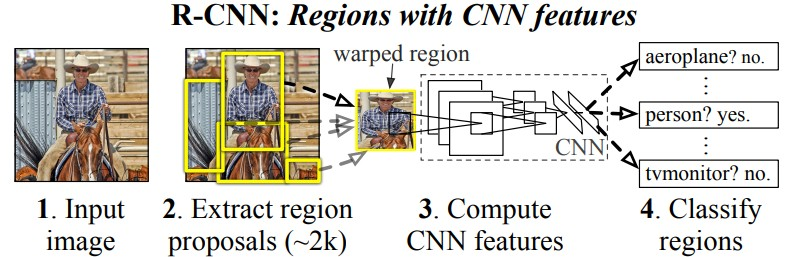
\includegraphics[width=\linewidth]{r_technologie/AI_assets/rcnn.png}
    \caption{Zarys działania modelu R-CNN. Źrodło: rozdział \emph{1. Introduction} w \cite{RCNN}}.
    \label{fig:R-CNN-schemat}
\end{figure}

Uprosczony schemat działania modelu R-CNN można przedstawić następująco:
\begin{enumerate}
    \item \textbf{Propozycja regionów:} Generowana jest pewna liczba regionów na obrazie wejściowym. Region to obszar obrazu, w którym potencjalnie może znajdować się wykrywany typ obiektu.
    \item \textbf{Pozyskanie cech regionów:} Każdy region jest odpowiednio przeskalowywany, a następnie przetwarzany za pomocą konwolucyjnej sieci neuronowej (CNN) w celu pozyskania wektora cech o stałym rozmiarze.
    \item \textbf{Klasyfikacja obiektów:} Na podstawie uzyskanego wektora cech odbywa się klasyfikacja każdego regionu -- przypisanie lub nie klasy obiektu do każdego regionu. Na koniec obszary regionów są poprawiane, aby lepiej obramowywały wykryty obiekt, a także usuwane są niektóre nachodzące na siebie regiony. Wynikowe regiony często określa się mianem prostokątów ograniczających (ang. \emph{bounding boxes}).
\end{enumerate}

 Koncepcja regionów znacznie zwiększyła dokładność detekcji (źródło: badania opisane w \cite{RCNN, Fast-RCNN, Faster-RCNN}), aczkolwiek modele z tej rodziny -- pomimo postępów w nowszych wersjach -- nadal były stosunkowo wolne ze względu na ich wieloetapowy schemat działania. Modele z rodziny R-CNN można okreslić mianem detektorów dwuetapowych (ang. \emph{two-stage detectors}), ponieważ w sposób niesymultaniczny wykonywały one dwa zadania:
\begin{enumerate}
    \item \textbf{Określenie lokalizacji:} propozycja regionów
    \item \textbf{Klasyfikacja:} pozyskanie cech regionów i klasyfikacja obiektów
\end{enumerate}

Opublikowanie w 2016 roku pierwszej wersji modelu YOLO (ang. \emph{You Only Look Once}) \cite{yolo_pierwszy_artykul} stało się istotnym wydarzeniem w dziedzinie wizji komputerowej. Podstawowym założeniem modelu jest jednoczesna realizacja zadań klasyfikacji i lokalizacji w ramch tylko pojedyńczego przejścia przez sieć konwolucyjną.  
Zaproponowane rozwiązanie było przykładem tzw. detektora jednostopniowego (ang. \emph{one-stage detector}). Jednostopniowość określa się jednoczesnym wykonywaniem klasyfikacji jak i określeniem lokalizacji.

\begin{figure}[H]
    \centering
    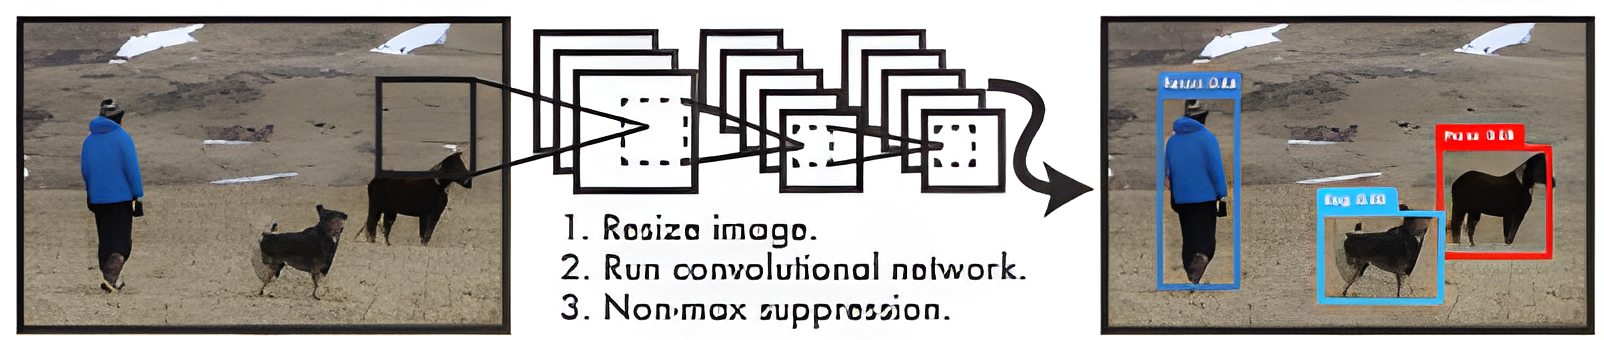
\includegraphics[width=\linewidth]{r_technologie/AI_assets/yolov1_1.png}
    \caption{Zarys działania modelu YOLOv1. Źrodło: rodział \emph{1. Introduction} w \cite{yolo_pierwszy_artykul}} .
    \label{fig:yolov1-schemat-dzialania}
\end{figure}
\begin{figure}[H]
    \centering
    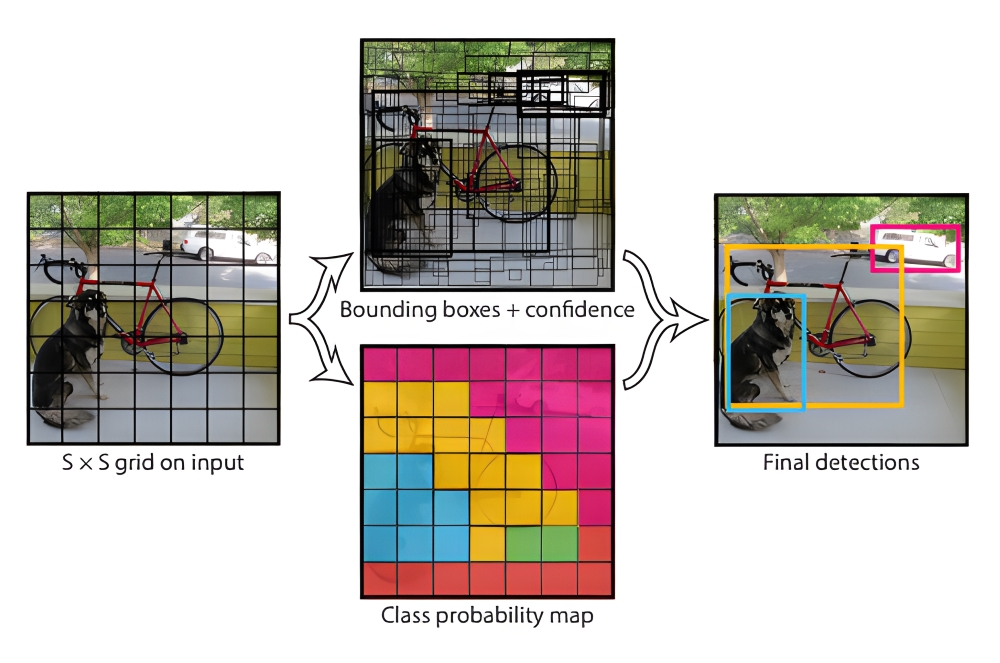
\includegraphics[width=\linewidth]{r_technologie/AI_assets/yolov1_2.jpg}
    \caption{Zarys działania CNN w modelu YOLO. Źrodło: rodział \emph{2. Unified Detection} w \cite{yolo_pierwszy_artykul}} .
    \label{fig:yolov1-schemat-dzialania-CNN}
\end{figure}


Na bazie \cite{yolo_pierwszy_artykul} ogólny schemat działania modelu YOLO (rysunek \ref{fig:yolov1-schemat-dzialania}), w tym CNN (rysunek \ref{fig:yolov1-schemat-dzialania-CNN}), można przedstawić następująco:
\begin{enumerate}
    \item \textbf{Dostosowanie obrazu wejściowego:} Obraz wejściowy jest przeskalowywany do określonego przez model rozmiaru.
    \item \textbf{Przetworzenie całego przeskalowanego obrazu przez CNN:} Na tym etapie odbywa się jednoczesna klasyfikacja oraz lokalizacja obiektów:
    \begin{enumerate}
        \item \textbf{Podział obrazu:} Obraz dzielony jest na siatkę rozmiaru $SxS$ dla pewnego $S$, tworząc $S^{2}$ komórek. 
        \item \textbf{Jednoczesna lokalizacja oraz klasyfikacja:} 
        \begin{enumerate}
            \item \textbf{Lokalizacja:} Dla każdej komórki szacowanych jest $B$ prostokątów ograniczających oraz określane są wyniki pewności (ang. \emph{confidence score}) dla każdego z nich. Wynik pewności wyraża z jakim prawdopodobieństwem model stwierdza wystąpienie obiektu oraz z jaką dokładnościa określa jego położenie przestrzenne.
            \item \textbf{Klasyfikacja:} Dla każdej komórki wyliczany jest zbiór rozmiarze $C$, gdzie $C$ odpowiada liczbie wykrywanych klas przez model. Pojedyńczy element zbioru odpowiada konkretnej klasie obiektu i zawiera wartość wyrażającą prawdopodobieństwo, iż obiekt w komórce należy do tej klasy obiektu. Prawdopodobiestwo to jest prawdopodobieństwem warunkowym -- opiera się na założeniu, że komórka przedstawia jakiś obiekt. 
        \end{enumerate}
        \item \textbf{Zakodowanie wyników obu operacji i przekazanie na wyjście CNN.}
    \end{enumerate}
    \item  \textbf{Eliminacja redundancji w wynikach CNN:} Usunięcie zbędnych prostokątów ograniczających, w tym takich nachodzących na inne. 
\end{enumerate}

Badania szybkości dotychczasowo dostępnych modeli -- w tym Faster R-CNN i YOLO -- w rozdziale \emph{4.1 Comparison to Other Real-Time Systems} \cite{yolo_pierwszy_artykul} pokazały znaczącą różnicę szybkości YOLO (YOLO i Fast YOLO) względem modeli z rodziny R-CNN na rzecz YOLO. Natomiast warto nadmienić, iż jednoczna poprawa szybkości wiązała się z redukcją dokładności modelu, co również zostało ukazane w w.w. badaniu.

Od momentu publikacji YOLO do momentu powstania niniejszego dokumentu (11 grudnia 2024) można wyróżnić co najmiej dziewięć kolejnych modeli. Modele te dokonywały różne zmiany w architekturze modelu pierwotnego, niemniej każdy z nich zachował podstawowe założenie realizacji zadań detekcji obiektów poprzez tylko pojedyńcze przejście przez CNN. 

Wizja komputerowa rozwija się w sposób dynamiczny. Na stan aktualny (grudzień 2024), w obecnym roku można wyróżnić co najmniej trzy nowe wersje modelu, w tym YOLO11 \cite{yolo11_ultralytics} (źródło: dokumentacja od firmy \emph{Ultralytics} \cite{yolo_docs}, podstrona \emph{/models}).
Ze względu na dynamikę rozwoju, w chwili wyboru wersjii dla niniejszego systemu, postanowiono rozważyć modele opublikowane do końca 2023r.. Na podstawie porównania modeli przedstawionych w \cite{yolo_docs} (podstrona \emph{/models/yolov8}) zdecydowano o wyborze technologii YOLOv8, a konkretniej modelu YOLOv8n. Zaletą YOLOv8 jest możliwość wyboru kilku podwersji o różnym rozmiarze modelu -- im mniejszy model, tym szybszy, a jednocześnie mniej dokładny.

\begin{figure}[H]
    \centering
    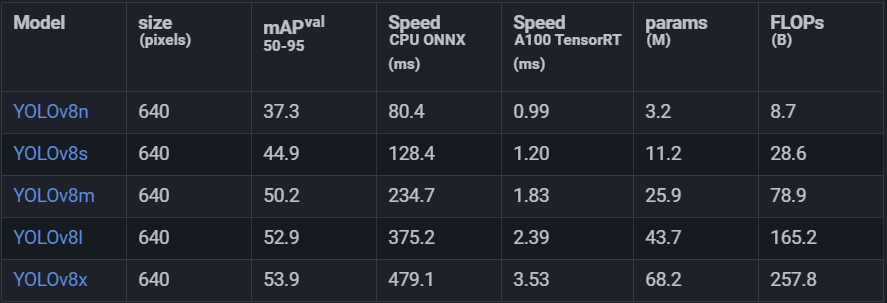
\includegraphics[width=\linewidth]{r_technologie/AI_assets/yolo8_sizes.png}
    \caption{Porównanie YOLOv8 o różnych rozmiarach. Wiersze posortowane wzlędem rozmiaru modelu. Źródło: \cite{yolo_docs}, podstrona \emph{/models/yolov8}}.
    \label{fig:yolo8-sizes}
\end{figure}

Ponieważ zaprojektowany system będzie operował na sprzęcie komputerowym (z naciskiem na kartę graficzną) posiadanym przez przeciętnego użytkownika, zdecydowano się postawić na szybkość modelu --- stąd wybór YOLOv8n. Zaletą YOLOv8 jest również duża liczba dostępnych klas obiektów dla niedostrojonego (ang. \emph{fine-tuned}) modelu -- jest ich 80. Zbiór dostępnych klas bazuje na zestawie danych COCO \cite{COCO_docs}, na którym przetrenowano model.

Podsumowując, użytym modelem w tym projekcie będzie podstawowa, niedostrojona wersja YOLOv8n. 



\subsection{Interfejs programistyczny do YOLO od firmy Ultralytics}
\label{chap:wprowadzenie-yolo_interjes}
Firma Ultralytics dostarcza interfejs programistyczny w formie pobieralnego modułu do języka Python \cite{Python_docs}. Poprzez różne tryby interfejsu istnieje możliwość wykorzystania różnego aspektu modelu. 

Tryby użytkowania to między innymi (źródło \cite{yolo_docs}, podstrona \emph{/modes}):
\begin{itemize}
    \item \textbf{train}: tryb do trenowania modelu na innych zestawach danych.
    \item \textbf{predict}: tryb inferencji. W kontekście YOLO, inferencja oznacza detekcję obiektów.
    \item \textbf{val}: tryb używany do ewaluacji przetrenowanego modelu.
\end{itemize}

W projeckie użyto trybu inferencji. Warto wspomnieć, iż dokumentacja \cite{yolo_docs} jest, na chwilę obecną (2 grudnia 2024), często pisana z perspektywy modelu YOLOv11. W praktyce wiele funkcji interfejsu działa również na innych wersjach modelu, w tym wersjach opartych na otwartym oprogamowaniu, a nie będących jednocześnie stworzonych przez autorów interfejsu. W przypadku użytych funkcji trybu inferencji, nie pojawiły się żadne problemy przy próbie użycia dla modelu YOLOv8n. 


\begin{lstlisting}[caption={Użycie trybu inferencji na przykładzie własnego kodu źródłowego.}, label={lst:inference_interface}]
from cv2.typing import MatLike
from ultralytics import YOLO
from ultralytics.engine.results import Results

from detector.yolo_settings import yolo_inference_config


class ImageProcessor:
    def __init__(self) -> None:
        self._detector = YOLO('yolo_models/yolov8.pt')

    def detect_objects(self, frame: MatLike) -> Tuple[Results, bool]:
        results = self._detector.predict(
            frame,
            conf=yolo_inference_config.confidence_threshold,
            device=yolo_inference_config.device,
            classes=yolo_inference_config.classes,
            verbose=yolo_inference_config.verbose
        ) # Returned type: list[Results] with only one element
        first_frame_result = results[0] # Get first (and only) frame from the list

        # Return detection results and also if there were any detected objects
        return first_frame_result, len(first_frame_result.boxes) > 0 

     def visualize_objects_presence(self, frame: MatLike, detections: Results) -> Tuple[MatLike, bool]:
        for box in detections.boxes:
            # Visualize bounding boxes
            x_min, y_min, x_max, y_max = box.xyxy[0] # coordinates
            # ...
\end{lstlisting}

Na bazie kodu \ref{lst:inference_interface}, inferencji można dokonać w następujący sposób:
\begin{itemize}
    \item \textbf{Zaimportowanie odpowiedniego obiektu z modułu ultralytics:} Aby skorzystać z usług interfejsu do komunikacji z modelami YOLO, wystarczy zaimportować i użyć obiekt \emph{YOLO} --- \emph{from ultralytics import YOLO}. Następnie należy stworzyć instancje wybranej przez użytkownika i dostępnej wersji YOLO, w tym wypadku YOLOv8 --- \emph{YOLO('yolo\_models/yolov8.pt')}.

    \item \textbf{Uzycie inferencji:} Inferencję można wykonać wywołaniem tylko jednej metody na wcześniej stworzonej instancji modelu --- metoda \emph{predict}. Pierwszy argument jest obowiązkowy, i jest źródłem obrazu. W tym przypadku jako argument podano klatkę obrazu pobraną przez bilbiotekę OpenCV -- typ \emph{MatLike}. Dalsze argumenty są opcjonalne. W przypadku niniejszego projektu użyto czterech z nich:
    \begin{itemize}
        \item \textbf{conf:} Parametr filtrujący. Jest to tzw. próg ufności (ang. \emph{confidence threshold}) wyrażony liczbą całkowitą z przedziału $[0.00, 1.00]$. Każda detekcja o wyniku pewności detekcji o wartości mniejszej od tego parametru jest odrzucana. 
        \item \textbf{device:} Określa urządzenie, na którym przeprowadzana jest inferencja. W projekcie tym użyto opcji \emph{'cuda'} --- inferencja przeprowadzana jest na procesorze graficznym firmy Nvidia.
        \item \textbf{classes:} Parametr filtrujący. Jest wyrażany listą indeksów klas obiektów. Określa klasy obiektów, których wykrycia model ma zwracać.
        Użycie tego parametru filtruje wyniki inferencji i zwraca wystąpienia tylko podanych klas. 
        \item \textbf{verbose:} Przyjmuje \emph{true} albo \emph{false}. Określa czy informacje na temat inferencji będą wysyłane do ustawionego strumienia wyjściowego. Parametr będzie zawsze ustawiony na \emph{false}.
    \end{itemize}
    Wyniki inferencji są zwracane jako typ \emph{Results}. Zawiera on m.in. liste prostokątów ograniczających. Pobranie koordynatów prostokąta dla pojedyńczego wyniku wymaga jedynie iteracji przez liste prostokątów (\emph{detections.boxes}) a następnie pobrania koordynatów z pojedyńczego prostokąta (\emph{box.xyxy[0]}).
\end{itemize}

W celu znalezienia informacji o pracy z obiektem wynikowym \emph{Results} oraz zapoznania się z resztą dostępnych parametrów inferencji rekomenduje się podstronę \emph{modes/predict} dokumentacji \cite{yolo_docs}.

Przedstawiony interfejs w przejrzysty i prosty sposób pozwala na użytkowanie modelu YOLOv8n. Jest to kolejny powód wybrania właśnie tej technologii. 

Niniejszy system umożliwia zmianę wartości progu ufności (\emph{conf}) oraz wykrywanych klas (\emph{classes}).

Warto również wspomnieć o parametrze \emph{imgsz}. Określa on rozmiar obrazu, na którym jest przeprowadzona detekcja obiektów. Obraz wejściowy jest przeskalowywany do tego rozmiaru. W projekcie wykorzystano domyślną wartość parametru, równą 640x640px.

\section{Język programowania}
Python jest to wysokopoziomowy, interpretowany język programowania. Jest on szeroko stosowany w dziedzinie sztucznej inteligencji, w tym wizji komputerowej. Za przykład może posłużyć opisany w rozdziale \ref{chap:wprowadzenie-yolo_interjes} interfejs. 

Implementacja języka generuje jednak problemy wydajnościowe. Ninejszy system jest opart na architekturze wielowątkowej. Tzw. GIL (ang. \emph{Global Interpreter Lock}) dopuscza możliwość by tylko jeden wątek programu mógł działać w tym samym czasie. Wprowadza to dodatkowy narzut mogący spowalniać aplikację. Istnieje podejście umożliwiające prawdziwe wykonanie współbieżne, ale jest one oparte na wieloprocesowości, co wiąże się z innym rodzajem narzutu, bardziej skomplikowaną komunikacją między procesami w porównaniu do wątków. Ostatecznie, szerokie zastosowanie języka w dziedzinie oraz wspomniany intefejs programistyczny zadecydowały o użyciu tego własnie języka. Informacje przedstawione w tym rozdziale wraz ze specyfikacją techniczną języka można znaleść w oficjalnej dokumentacji \cite{Python_docs}. 

\section{Przetwarzanie obrazów i pobór klatek ze strumienia wideo}
Niniejszy projekt zakłada pobór kolejnych klatek obrazu ze źródła wideo oraz rózne manipulacje na obrazie, w tym przeskalowanie obrazu oraz narysowanie prostokątów ograniczających wraz z podpisami wykrytych klas obiektów. Wszystkie te zadania mają implementację w bibliotece OpenCV. Bilbioteka posiada swoją wersje również jako moduł dla języka Python o nazwie \emph{cv2}. Bilbioteka ta została wybrana ze względu na prostą integrację z Pythonem, realizacje przedstawionych wyżej zadań oraz optymalizację tych zadań. Dokumentacja biblioteki: \cite{OpenCV_docs}



\section{Graficzny interfejs użytkownika}
Zadania, które musi spełniać GUI to:
\begin{itemize}
    \item \textbf{Panel sterowania:} Dostarczenie interfejsu do integracji użytkownika z silnikiem detekcji obiektów, w tym możliwość zmiany parametrów detektora obrazu oraz ustawienie źródła wideo (kamera lub nagrany film). Zarządzanie wyświetlaniem klatek obrazu -- wywołanie funkcji odpowiedzialnej za wyświetlenie klatki".
    \item \textbf{Wyświetlacz: } Wyświetlanie przetworzonych klatek obrazu.
\end{itemize}

Panel sterowania nie jest skomplikowany, dlatego też nie wymaga użycia złożonej technologii. Z kolei wyświetlacz wymaga tylko jednej funkcji, natomiast musi być ona jak najlepiej zomptymalizowana. Biorąc pod uwage te czynniki zdecydowano się na użycie dwóch różnych technologii i zintegrowanie ich w jeden graficzny interfejs użytkownika.

Za panel sterowania, odpowiada moduł tkinter -- GUI z biblioteki standardowej języka Python. Jest to dobrze udokumentowane i lekkie rozwiązanie. W przypadku wyświetlania, ponownie zdecydowano się na użycie bilbioteki OpenCV, a dokładniej funkcji \emph{cv2.imshow()}. Jest to funkcja specjalnie zoptymalizowana pod wyświetlanie i, tak jak jak to zostało wspomniane, jedyna konieczna do wyświetlenia obrazu.
Zrezygnowano z użycia tkinter jako wyświetlacza, ponieważ nie jest on zoptymalizowany pod wyświetlanie klatek z dużą częstotliwością. 

Dokumentacja do modułu tkinter zawiera się w dokumentacji języka Python \cite{Python_docs}.

\begin{figure}[H]
    \centering
    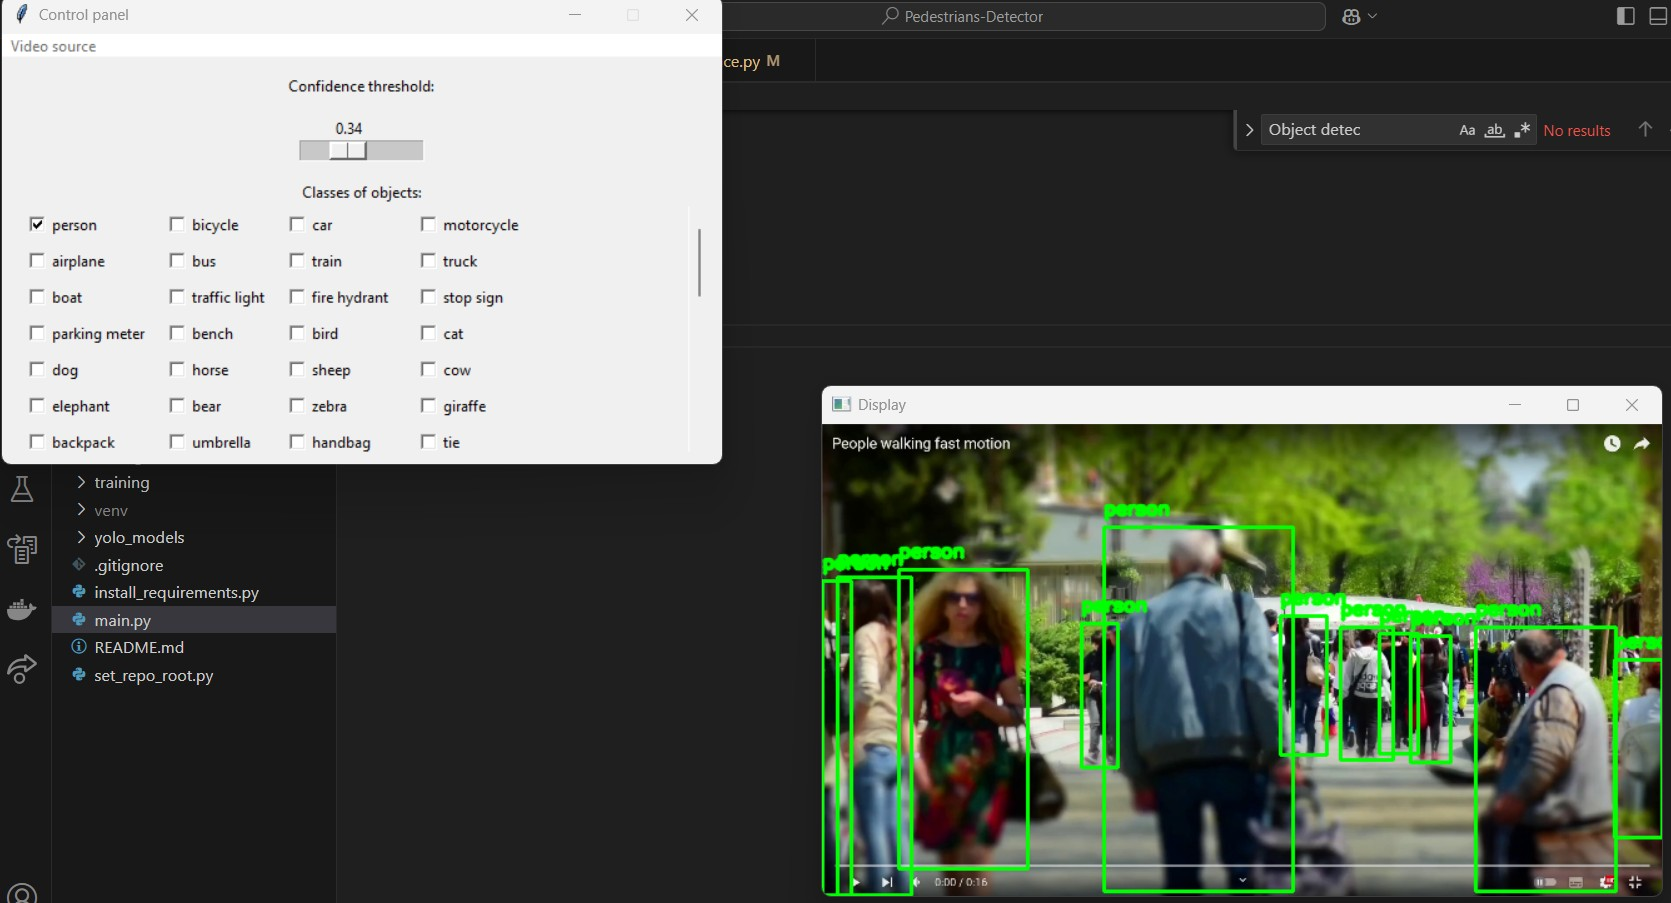
\includegraphics[width=\linewidth]{r_technologie/GUI_assets/mockup.jpg}
    \caption{Wygląd GUI w projekcie: panel sterowania -- w lewym górnym rogu, wyświetlacz -- w prawym dolnym rogu}
    \label{fig:technologies-GUI}
\end{figure}
\chapter{Projekt i implementacja systemu}
\label{sec:implementacja-systemu}
W rozdziale tym opisano szczegóły implementacji systemu. 
Zdefiniowane zostały funkcje jakie oprogramowanie ma spełniać.  
System opisano na poziomie klas, ich przeznaczenia oraz integracji między nimi. Zagłębiono się również w  decyzje architektoniczne wprowadzono w celu optymalizacji. 
Ponadto zaprezentowano przykład użycia systemu z persepktywy użytkownika.

\section{Wymagania funkcjonalne i założenia systemowe}
Projektowany system będzie służył synchronizacji różnych wymagań funkcjonalnych opisanych w niniejszym rozdziale. Będzie on wykonany w postaci oprogramowania. 
Oprogramowanie będzie wytworzone w formie aplikacji desktopowej, dostępnej na system operacyjny Windows 11. Aplikacja ta musi posiadać graficzny interfejs użytkownika (GUI) składający się z panelu sterującego oraz wyświetlacza. 
Oprogramowanie ma obługiwać jedną z dostępnych (niewykorzystywanych przez inne procesy) kamer podłączonych do komputera. Lista dostępnych kamer jest określana jednorazowo przed pojawieniem się GUI na ekranie. Dlatego w przypadku chęci użycia kamery podłączonej w trakcie wykonywania programu należy zamknąć aplikację (panel sterowania GUI) i uruchomić ją ponownie.

Na podstawie powyższych założeń, kolejne wymagania fukncjonalne można podzielić na dwa bloki: pierwszy (logiczny), drugi (wpływający na stan GUI). Na bazie pierwszego bloku system realizuje następujące funkcje:
\begin{itemize}
    \item Pobiera klatki obrazu z kamery.
    \item Zmniejsza rozmiar klatki, jeżeli jest on większy niż ekran monitora komputera.
    \item Wykrywa obiekty na podanej klatce obrazu.
    \item Przygotowuję klatkę obrazu do wyświetlenia -- wizuallizuje lokalizację obiektów bazując na wynikach detekcji, jeżeli znajdują się w nich wykrycia.
    \item Alarmuje dźwiękowo użytkownika, jeżeli obiekty zostały wykryte.
    \item Synchronizuje wyżej wypunktowane funkcje.
\end{itemize}

Na bazie drugiego bloku system:
\begin{itemize}
        \item Wyświetla przygotowane klatki obrazu w wyświetlaczu GUI.
        \item Umożliwia użytkownikowi wyłączenia źródła wideo (wyłączenia wyświetlacza) w panelu sterowania GUI.
        \item Umożliwia użytkownikowi ustawienie progu ufności detekcji (próg ufności opisany w rozdziale \ref{chap:wprowadzenie-yolo_interjes}) obiektów w panelu sterowania GUI.
        \item Umożliwia użytkownikowi ustawienie wykrywanych klas obiektów ze zdefiniowanego zbioru klas w panelu sterowania GUI.
        \item Umożliwia użytkownikowi wybór kamery jako źródło wideo z dostępnych kamer wejściowych w panelu sterowania GUI.
        \item Generuje listę dostępnych kamer przed wyświetleniem GUI.
\end{itemize}

System musi zorganizować funkcje w odpowiednie moduły i odpowiednio je synchronizować. Założoną architekturą systemu jest architektura wielowątkowa. 
\section{Architekrura systemu}

\section{Implementacja systemu na poziomie klas}
Oprogramowanie podzielono na sześć klas: \emph{App}, \emph{VideoCapture}, \emph{YoloInferenceConfig}, \emph{ImageProcessor}, \emph{VideoProcessingEngine} oraz \emph{GUI}.

\emph{App} jest punktem centralnym aplikacji. W tym miejscu rozpoczyna się program i tworzone są instancję pozostałych pięciu klas. Pierwszym zadaniem klasy jest utworzenie obiektów pozostałych klas. Następnie klasa ta służy jako interfejs do komunikacji między modułem interfejsu graficznego użytkownika (\emph{GUI}), a sekcją logiczną -- w tym do pobrania informacji o liście dostępnych kamer (\emph{VideoCapture}), ustawienia parametrów inferencji detektora (\emph{ImageProcessor}) oraz do komunikacji z silnikiem przetwarzania wideo (\emph{VideoProcessingEngine}).
Ponadto, klasa ta implementuje metodę, która uruchamia alarm dźwiękowy (\emph{{play\_audio\_alert}}). 
 
\emph{VideoCapture} służy do obługi źródła wideo. Klasa dostarcza kluczową metode, \emph{get\_frame}, której wywołanie zwraca informację o tym czy źródło wideo nadal jest dostępne oraz najnowszą dostępną klatkę z kamery. Ponadto warto wyróżnić metodę do pozyskania dostępnych do użycia kamer (\emph{get\_available\_sources}). Klasa ta zawiera również metody \emph{start\_capture} oraz \emph{end\_capture} odpowiedzialne kolejno za ustanowienie połączenia z podaną jako argument kamerą oraz zwolnienia tego połączenia. 

\emph{YoloInferenceConfig} jest to klasa, której głównym celem jest przechowywanie parametrów inferencji (progu ufności oraz wykrywanych klas) oraz dostarczenie metod do zmiany tych parametrów. Klase utworzono dla zachowania większej czytelności kodu w \emph{ImageProcessor}, dlatego też jest ona dziedziczona przez \emph{ImageProcessor} właśnie. W chwili uruchomienia aplikacji, klasa jest inicjalizowana domyślnymi parametrami: próg ufności równy $0.5$ oraz \emph{człowiek} jako wykrywana klasa. 

\emph{ImageProcessor} służy do przetwarzania oraz analizy obrazu. Kluczowe trzy metody to \emph{detect\_objects}, zwracająca liczbe wykrytych obiektów oraz wyniki detekcji na podstawie podanej klatki obrazu; \emph{visualize\_objects\_presence}, która na postawie w.w. wyników detekcji, rysuję prostokąty ograniczające dookoła wykrytych obiektów; \emph{fit\_frame\_into\_screen}, która zmniejsza rozmiar podanej klatki, jeżeli jest większa niż rozmiar ekranu monitora podłączonego do komputera.

\emph{VideoProcessingEngine} stworzono w celu koordynacji i rozplanowania wszystkich zadań koniecznych do uzyskania kolejnych klatek obrazu, gotowych do wyświetlenia w graficzym interfejsie użytkownika, oraz realizacji celu alarmowania dźwiękowego użytkownika, kiedy jest to konieczne. Zbiór zadań zawiera pobranie klatki z kamery, detekcję obiektów, przetworzenie klatki w celu wizualizacji obiektów, alarmowanie dźwiękowe użytkownika oraz umieszczenie klatki w buforze wyjściowym. Zadania te nie mają implementacji w samej klasie i są metodami wywoływanymi z innych klas (\emph{App}, \emph{ImageProcessor} oraz \emph{VideoCapture}).
Podsumowując tę część opisu, jest więc klasa realizująca moduł silnika przetwarzania wideo opisanego w rodziale \ref{chap:architektura}. Klasa ta również dostarcza metody do wznowienia (\emph{set\_video\_source}) lub zatrzymania (\emph{remove\_video\_source}) kolejnych wykonań sekwencji opisanych w w.w. rozdziale, wywołując przy tym m.in. odpowiednio metody \emph{VideoCapture} \emph{start\_capture} oraz \emph{end\_capture}.  

\emph{GUI} to graficzny interfejs użytkownika aplikacji. Składa się on z wyświetlacza klatek obrazu oraz panelu sterowania. Tak jak to wcześniej wspomniano, używa on \emph{App} w celu komunikacji z resztą klas. Tyczy się to zarówno komunikacji dwustronnej z \emph{ImageProcessor}, potrzebnej do pobrania parametrów detektora oraz ich ustawnienia w panelu sterowania, komunikacji dwustronnej z \emph{VideoProcessingEngine} w celu pobrania klatki z bufora wyjściowego oraz kontroli sekwencji oraz komunikacji jednostronnej z \emph{VideoCapture} w celu pobrania listy dostępnych kamer.

Opisane zależności komunikacyjne między klasami, w tym typy połączeń między nimi (kompozycja, agregacja, dziedziczenie) zilustrowano uprosczonym diagramem UML na rysunku \ref{fig:uprosczony-diagram-klas}. 
%Pełen diagram UML przedstawiono na rysunku \ref{fig:diagram-klas}. 

\begin{figure}[H]
    \centering
    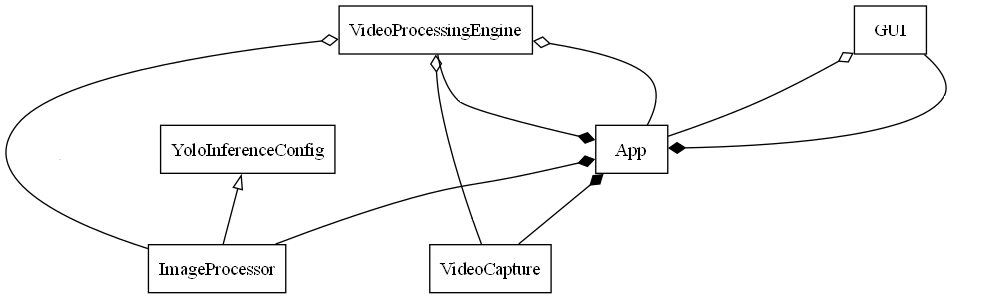
\includegraphics[width=\linewidth]{r_implementacja/klasy/simplified_classes.png}
    \caption{Uprosczony diagram klas UML (bez metod i pól) wygenerowany przez bilbiotekę \emph{pylint}.}
    \label{fig:uprosczony-diagram-klas}
\end{figure}

Tak jak wspomniano klasa \emph{YoloInferenceConfig} nie jest instancjowana -- programowe użycie jej pól odbywa się wewnątrz \emph{ImageProcessor}, zaś jej metody są wywoływane poprzez obiekt klasy \emph{ImageProcessor}. Jest to umożliwione dzięki dziedziczeniu \emph{YoloInferenceConfig} przez \emph{ImageProcessor}.

\emph{App} jako punkt startowy aplikacji tworzy w swoim konstruktorze obiekty klas \emph{VideoCapture}, \emph{ImageProcessor}, \emph{VideoProcessingEngine} oraz \emph{GUI}. Istnienie tych obiektów jest zależne od istnienia klasy App -- z perspektywy UML jest to kompozycja. Nazwy tych obiektów to według kolejności: \emph{\_image\_processor}, \emph{\_video\_capture}, \emph{\_video\_processing\_engine} oraz \emph{\_gui}. Następnie, plik główny programu (\emph{main.py}) wywołuję metodę \emph{run}. Metoda ta uruchamia silnik generacji klatek (\emph{self.\_video\_processing\_engine.run()}) oraz wyświetla graficzny interfejs użytkownika \emph{self.\_gui.show()}. Po zamknięciu GUI wykonywana jest ostatnia instrukcja -- wyłączająca silnik generacji klatek (\emph{self.\_video\_processing\_engine.shutdown()}). Opisane użycie zareprezentowano fragmentem kodu w listingu \ref{lst:app-instancjowanie}. 

\begin{lstlisting}[caption={Tworzenie obiektów klas wewnątrz \emph{App} oraz uruchomienie w niej różnych sekcji aplikacji.}, label={lst:app-instancjowanie}]
class App:
    # Konstruktor App
    def __init__(self) -> None:
        # ... reszta kodu
        # Tworzenie obiektow klas:
        self._video_capture = VideoCapture()
        self._image_processor = ImageProcessor()
        self._video_processing_engine = VideoProcessingEngine(self._video_capture, self._image_processor, self)
        self._gui = GUI(self)
        # reszta kodu ...

    # Metoda uruchamiajaca poszczegolne sekcje aplikacji
    def run(self) -> None:
        self._video_processing_engine.run()
        self._gui.show()
        self._video_processing_engine.shutdown()
\end{lstlisting}

Tak jak wspomniano w opisach klas, \emph{App} jest interfejsem komunikacyjnym między \emph{GUI}, a resztą klas potrzebnych \emph{GUI}. Do \emph{GUI} przekazywana jest referencja (obiekt) \emph{App}, z której poziomu utworzono obiekt \emph{GUI}. W celu pobrania bądź zmiany informacji w innych modułach \emph{GUI} wywołuje metody \emph{App} poprzez tę referencję. Z perspektywy \emph{GUI} jest to agregacja. Taki sam typ relacji dotyczy również \emph{VideoProcessingEngine} do \emph{App}, której referencje \emph{VideoProcessingEngine} wykorzystuje do wywołania metody alarmującej dźwiękowo użytkownika. Agregacja w \emph{VideoProcessingEngine} występuje również względem \emph{ImageProcessor} oraz \emph{VideoCapture}.


\section{Szczegóły implementacyjne}
W sekcji tej opisano implementacje wielowątkowego podejścia architektonicznego. Przedstawiono argumenty za wybraniem tego typu architektury, rozwiazanie problemów przez nią wywoływanych oraz uzasadnienie innych działań zastosowanych w celu poprawy wydajności systemu.  

Pierwsza iteracja oprogramowania była oparta na architekturze jednowątkowej. Sekwencyjnie wykonywano kolejne metody w nieskończonej pętli: pobór klatki z kamery, detekcja obiektów, alarmowanie dźwiękowe, wizualizacja obiektów oraz wyświetlenie klatki w wyświetlaczu graficznego interfejsu użytkownika.

Na tym etapie rodziału warto pochylić się nad działaniem modułu graficznego użytego w klasie \emph{GUI} --- tkinter. 
Jest on podstawą i jedyną wykorzystywaną technologią w implementacji panelu sterowania. Moduł ten dostarcza graficzne komponenty takie jak suwak, wykorzystany do zmiany progu ufności, przewijaną sekcja z polami wyboru wykrywanych klas obiektów, oraz menu do wyboru źródła wideo. 

Aby móc użytkować interfejs na bazie modułu, wymagane jest wywołanie głównej pętli tkinter (ang .\emph{mainloop}). Pętla opiera się ona na architekturze wydarzeniowej (ang. \emph{event-driven architecture}) działającej w ramach jednego, głównego wątku aplikacji. Poprzez wydarzenie rozumie się zdefiniowaną w module integrację z komponentem np. kliknięcie na przycisk. Zadaniem pętli jest zareagowanie na wydarzenia w sposób zfefiniowany przez moduł (np. wypełnienie przycisku kolorem po kliknięciu) oraz wykonanie kodu, który programista podłączył pod dane wydarzenia (np. wywołanie metody ustawiającej źródło wideo). Przykład na bazie kodu źródłowego pokazano w listingu \ref{lst:tkinter-event-loop}.


\begin{lstlisting}[caption={Podłączenie metod pod wydarzenia oraz zainicjalizowanie pętli głównej w module tkinter.}, label={lst:tkinter-event-loop}]
def GUI:
    # Metoda tworzaca panel sterowania
    def _initialize_control_panel(self) -> None:
        self._root = tk.Tk() # Utworzenie aplikacji (okna) tkinter
        # Utworzenie menu do wyboru zrodla wideo:
        self._menubar = tk.Menu(master=self._root)
        self._root.config(menu=self._menubar)
        self._initialize_video_source_menu()
        # reszta kodu metody ...

    # Metoda tworzaca menu z przyciskami do wyboru zrodla wideo 
    def _initialize_video_source_menu(self) -> None:
        self._source_menu = tk.Menu(master=self._menubar, tearoff=0)
        self._selected_video_source_id = tk.IntVar()

        sources = self._frame_generator.get_available_sources()
        for source_name in sources:
            # Stworzenie pojedynczego przycisku:
            self._source_menu.add_radiobutton(
                label=source_name,
                variable=self._selected_video_source_id,
                value=sources[source_name],
                # Podlaczenia zaprogramowanej funkcji do ustawienia zrodla wideo do wywolania po nacisnieciu przycisku:
                command=lambda source_index=sources[source_name]: self._on_video_source_select(source_index) 
            )

        self._selected_video_source_id.set(NO_VIDEO)
        self._menubar.add_cascade(menu=self._source_menu, label='Video source')

    # Metoda uruchamiajaca GUI (inizjalizuje petle tkinter)
    def show(self) -> None:
        # ... kod poprzedzajacy
        self._root.mainloop()
        # reszta kodu... (zostanie wykonana po zakonczeniu petli)

\end{lstlisting}

Z perpektywy programistycznej, instrukcje wywołane po instrukcji inicjalizacji zostaną wykonane dopiero po jej zakończeniu -- zamknięciu przez użytkownika okna aplikacji. Generuje to konieczność wywołania sekcji logicznej aplikacji przed rozpoczęciem pętli. Jest to jednak problematyczne, ponieważ sekcja ta musi stać się częścią mechanizmu tej pętli właśnie. Oferowanym rozwiązaniem jest funkcja również zawarta w tkinter -- \emph{after}. Funkcja ta przyjmuje liczbe całkowitą określającą czas w milisekundach, po którym zostanie wykonana metoda przekazana jako drugi argument tej funkcji. 

Użycie \emph{after} nie blokuje wykonania kolejnych instrukcji w kodzie dlatego też może być bezpiecznie użyte w ramach aplikacji tkinter. Zaprogramowanym sposobem użycia jest wywołanie metody do komunikacji z sekcją logiczną \emph{\_update\_frame}. Istotą tego rowiązania jest zawarcie w kodzie tej metody najpierw obsługi sekcji logicznej oraz późniejsze wywołanie tej samej metody przy użyciu funkcji \emph{after}. Nieblokujący mechanizm \emph{after} unika nieskończonej rekurencji prowadzącej do pojawienia się wyjątków pamięciowych systemu operacyjnego. Mechanizm wyświetlania przy użyciu opisanych funkcji opisano w listingu \ref{lst:tkinter-after}.

\begin{lstlisting}[caption={Wyświetlanie klatek obrazu w GUI przy pomocy modułu tkinter.}, label={lst:tkinter-after}]
AFTER_DELAY = 1 # Czas w milisekundach. Najmniejsze mozliwe ustawienie. 
class GUI:
    # Konstruktor klasy
    def __init__(self, communication_interface: App) -> None:
        # Ustawienie interfejsu do komunikacji z sekcja logiczna oprogramowania, w tym poboru klatek z kamery:
        self._communication_interface = communication_interface
        # reszta kodu ...

    # Metoda do uruchomienia GUI
    def show(self) -> None:
        self._root.mainloop() # inicjalizacja petli tkinter

    # Metoda uruchamiana w po ustawieniu kamery w panelu sterowania
    # Sluzy do rozpoczecia komunikacji z warstwa logiczna w celu poboru klatki do wyswietlenia  
    def _start_displaying(self) -> None:
        self._is_displaying = True
        cv.namedWindow('Display', cv.WINDOW_NORMAL) # Stworzenie okna wyswietlacza
        cv.moveWindow('Display', 0, 0)
        self._update_frame()

    # Metoda uruchamiana po zakonczeniu strumienia wideo
    # Sluzy zakonczeniu wyswietlania (zakonczenie poboru klatek)
    def _stop_displaying(self) -> None:
        self._is_displaying = False
        cv.destroyAllWindows() # Zniszczenie okna wyswietlacza

    def _update_frame(self) -> None:
        if not self._is_displaying:
            self._stop_displaying()
            return

        # Pobranie klatki (frame) oraz informacji o tym czy kamera dalej dziala (is_capture_on):
        is_capture_on, frame =  self._communication_interface.get_processed_frame()

        if is_capture_on:
            if frame is not None:
                self._show_frame(frame)
            # Jezeli kamera dziala, mechanizm kontunuowany:
            self._root.after(AFTER_DELAY, self._update_frame)
        else:
            self._frame_generator.set_video_source(NO_VIDEO)
            self._selected_video_source_id.set(NO_VIDEO)
            self._stop_displaying()

    # Metoda wywolywana do wyswietlania klatki obrazu
    def _show_frame(self, frame: MatLike) -> None:
        frame = cv.cvtColor(frame, cv.COLOR_BGR2RGB)
        cv.imshow('Display', frame) # Wyswietlenie klatki
\end{lstlisting}

Użycie interfejsu w celu pobrania klatki (\emph{self.\_communication\_interface.get\_processed\_frame()}) pozwoliło oddzielić sposób pozyskania klatki od architektury komunikacyjnej między sekcją GUI, a sekcją logiczną oraz zachować taki sam kod klasy \emph{GUI} dla następnych iteracji systemu. W przypadku iteracji jednowątkowej użycie metody interfejsu wywoływało następującą sekwencję kroków: pobór klatki z kamery; zmniejszenie rozmiaru klatki, tak aby zmieściła się na ekranie komputera; detekcja obiektów; alarmowanie dźwiękowe oraz wizualizacja prostokątów ograniczających w przypadku wykrycia obiektów; zwrócenie przetworzonej klatki obrazu.

Długa sekwencja zadań oraz czasochłonność niektórych operacji (np. detekcji obiektów) blokowała odświeżanie oraz dostęp do funkcji komponentów GUI, czyniąc go oraz cały system nieresposywnym i powolnym. W celu poprawy optymalizacji nie zdecydowano się zmienić ustawionego, minimalnego czasu, po którym następują kolejne wykonania \emph{\_update\_frame}, ponieważ ryzykowano by utratą wiekszej ilości pobieranych klatek -- kluczowych dla alarmowania użytkownika -- pomimo poprawy responsywności interfejsu graficznego.

Pierwszym podjętym krokiem w celu poprawy wersji jednowątkowej było przeniesienie wykonania inferencji (detekcji) z CPU na GPU. Parametr do tego użyty był opisany w rodziale \ref{chap:wprowadzenie-yolo_interjes}. Poprawiło tym znacznie wydajność uzyskania finalnej klatki, aczkolwiek GUI nadal borykało się z problemem responsywności. Postanowiono więc zmienić architekturę na wielowątkową. Podejściem takim osiągniąto zamierzone rezultaty -- GUI osiągneło zadowalający poziom responsywności przy zachowaniu satysfakcjonującej wydajności (opisanej w rozdziale \ref{chap:test-szybkosci}, testów szybkości systemu). 



\chapter{Test szybkości systemu}
\label{chap:test-szybkosci}
W tym rozdziale opisano badanie sprawdzające ile czasu zajmuje systemowi wykonanie wszystkich zadań koniecznych do wyświetlenia przetworzonej klatki obrazu. Porównano w nim m.in. wpływ rozdzielczości kamery. Pomiary zrealizowano dla trzech różnych ustawień rozdzielczości tej samej kamery: 640x360px, 640x480px i 1280x720px.
Według informacji pobranych z kamery za pomocą biblioteki OpenCV, operuje ona w 30 klatkach na sekundę, co daje około 33.33 milisekund na pojedyńczą klatkę. Liczba klatek użytych do testu to pięć tysięcy dla każdej rodzielczości.
Test wykonano na komputerze wyposażonym w kartę graficzną \emph{NVIDIA GeForce GTX 1650} i procesor \emph{Intel Core i5-8300H 2.30GHz}.

Poprzez czas potrzebny do wyświetlenia klatki rozumie się szereg czynności. Jest to proces rozpoczynający się od pobrania klatki z kamery, następnie detekcji obiektów oraz przetworzenia klatki w celu oznaczenia wykrytych obiektów, a kończący się poprzez wyświetlenie przetworzonej klatki obrazu przez graficzny interfejs użytkownika. 

W teście zmierzono całkowity czas do wyświetlenia wszystkich klatek oraz czas potrzebny do wyświetlenia pojedyńczej klatki (pięć tysięcy pomiarów na każdą rozdzielczość). Czas zmierzono poprzez pobranie w dwóch punktach -- początkowym i końcowym -- kodu źródłowego aktualnego czasu w systemie operacyjnym i obliczeniu różnicy jaka wystąpiła między tymi punktami. 

Dla pomiaru czasu całkowitego punkt początowy umiesczono po wyświetleniu przez GUI pierwszej klatki (klatka zerowa --- niewliczona do pomiaru). Punkt końcowy zmierzono po wyświetleniu ostatniej klatki.
Dla pojedyńczego pomiaru punkt początkowy jest taki sam dla pierwszej uwzględnionej klatki. Punkt końcowy jest ustawiany po wyświetleniu następnej klatki, w tym momencie też punkt końcowy staje się punktem początkowym dla pomiaru dla kolejnej klatki.
Pomiary czasu całkowitego dla zbadanych rozdzielczości kamery przedstawiono w tabeli \ref{tab:czas-calkowity-5000klatek}. Tabela uwzględnia zmierzony czas całkowity oraz obliczony na jej podstawie średni czas na klatkę oraz liczbę klatek na sekundę (FPS). Średni czas na klatkę obliczono poprzez podzielienie liczby klatek (5000) przez czas całkowity, natomiast FPS poprzez podzielenie liczby klatek przez czas całkowity.  
\begin{table}[H]
\centering
\caption{Pomiar czasu potrzebnego do wyświetlenia 5000 klatek.}
\begin{tabular}{|c|c|c|c|}
\hline
Rozdzielczość & Średni czas na klatke {[}ms{]} & Czas całkowity {[}s{]} & FPS   \\ \hline
640x360px     & 33.34                          & 166.69                 & 30    \\ \hline
640x480px     & 33.48                          & 167.42                 & 29.87 \\ \hline
1280x720px    & 33.58                          & 167.89                 & 29.78 \\ \hline
\end{tabular}
\label{tab:czas-calkowity-5000klatek}
\end{table}

Pomiary czasu całkowitego pokazały brak wpływu rozdzielczości kamery na szybkość systemu. Przyczynę takiego zachowania można upatrywać w optymalizacji YOLOv8, bowiem model ten przed rozpoczęciem detekcji skaluje obraz wejściowy do stałego rozmiaru -- do domyślnego rozmiaru lub ustawionego przez programistę parametrem inferencji \emph{imgsz} -- i wykonuje detekcję na przeskalowanym obrazie. Z racji braku opisu w dokumentacji modelu \cite{yolo_docs}, potwierdzenie istnienia tego mechanizmu opisano jako odpowiedź do pytania zadanego na forum, które jest umieszczone razem z repozytorium kodu modelu \cite{github_imgsz}.

Interesującą obserwacją jest również osiągnięcie liczby klatek na sekundę równej FPS kamery. Powodem może być np. wariacja w liczbie realnych klatek na sekundę dostarcznych przez kamerę lub OpenCV (np. powtórzenie odczytu tej samej klatki).

Pomiary czasu całkowitego nie obrazują jednak potencjalnych odchyleń od średniej. Dlatego też postanowiono zilustrować pojedyńcze pomiary. Wykresy punktowe na rysnkach \ref{fig:czas-punktowy1}, \ref{fig:czas-punktowy2} i \ref{fig:czas-punktowy3} przedstawiają te pomiary i zestawiają je wraz z odpowiadającym średnim czasem z tabeli \ref{tab:liczba-klatek}. Aby sprawdzić różnicę w odchyleniach pomiędzy rozdzielczościami, dane z powyżej wspomnianych wykresów scalono na wykresie na ryskunku \ref{fig:czas-punktowy-all}.  


\begin{figure}[H]
    \centering
    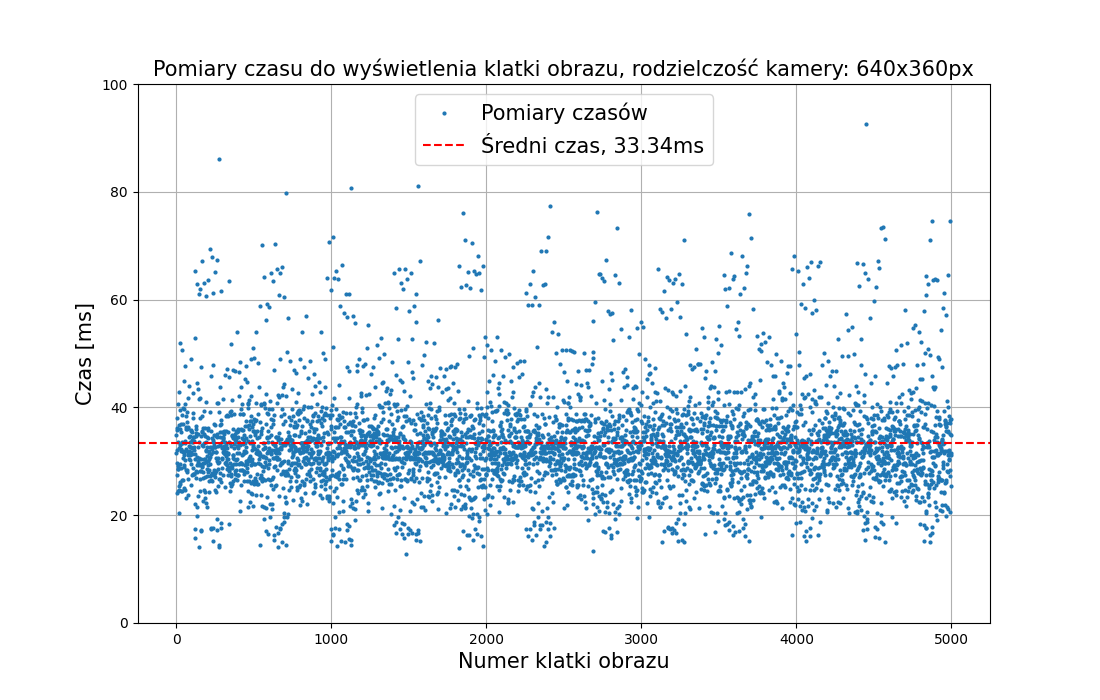
\includegraphics[width=\linewidth]{r_test_szybkosci/punkty/1.png}
    \caption{Wykres punktowy dla rodzielczości 640x360px przedstawiający pomiary czasu do wyświetlenia obrazu dla każdej klatki.}
    \label{fig:czas-punktowy1}    
\end{figure}

\begin{figure}[H]
    \centering
    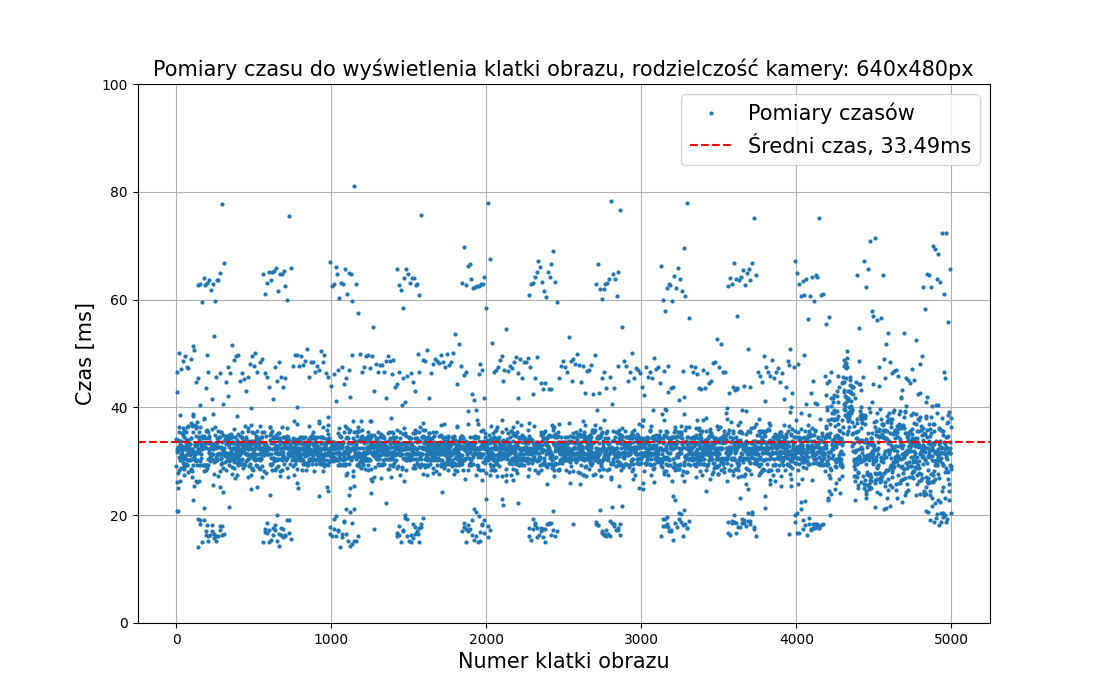
\includegraphics[width=\linewidth]{r_test_szybkosci/punkty/2.png}
    \caption{Wykres punktowy dla rodzielczości 640x480px przedstawiający pomiary czasu do wyświetlenia obrazu dla każdej klatki.}
    \label{fig:czas-punktowy2}    
\end{figure}

\begin{figure}[H]
    \centering
    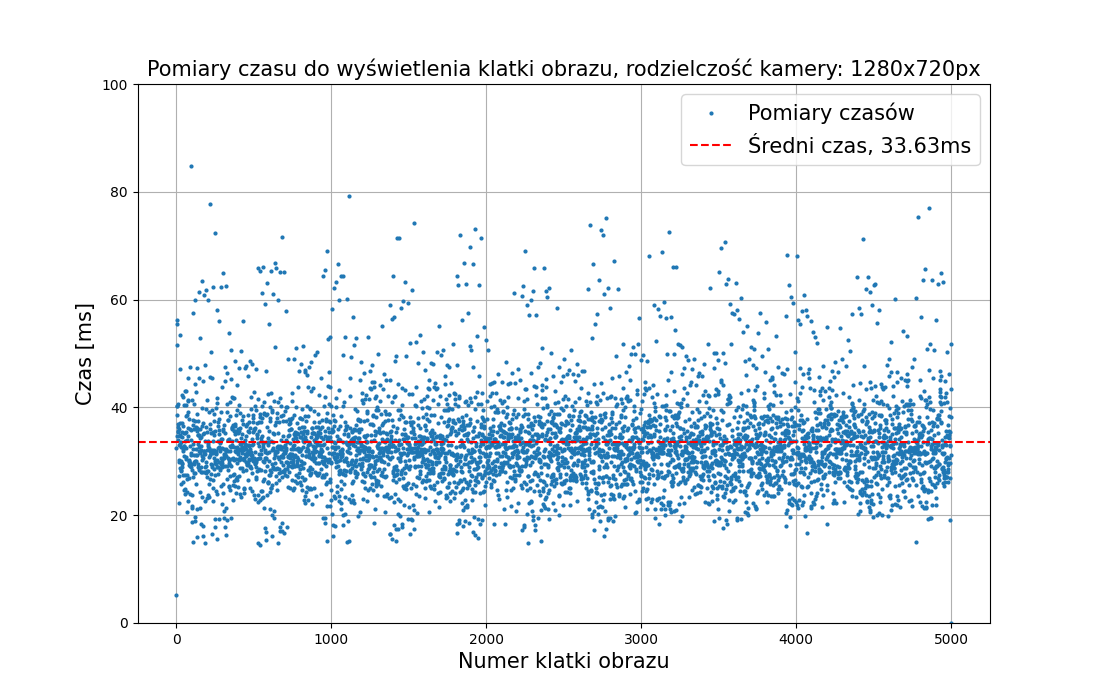
\includegraphics[width=\linewidth]{r_test_szybkosci/punkty/3.png}
    \caption{Wykres punktowy dla rodzielczości 1280x720px przedstawiający pomiary czasu do wyświetlenia obrazu dla każdej klatki.}
    \label{fig:czas-punktowy3}    
\end{figure}

\begin{figure}[H]
    \centering
    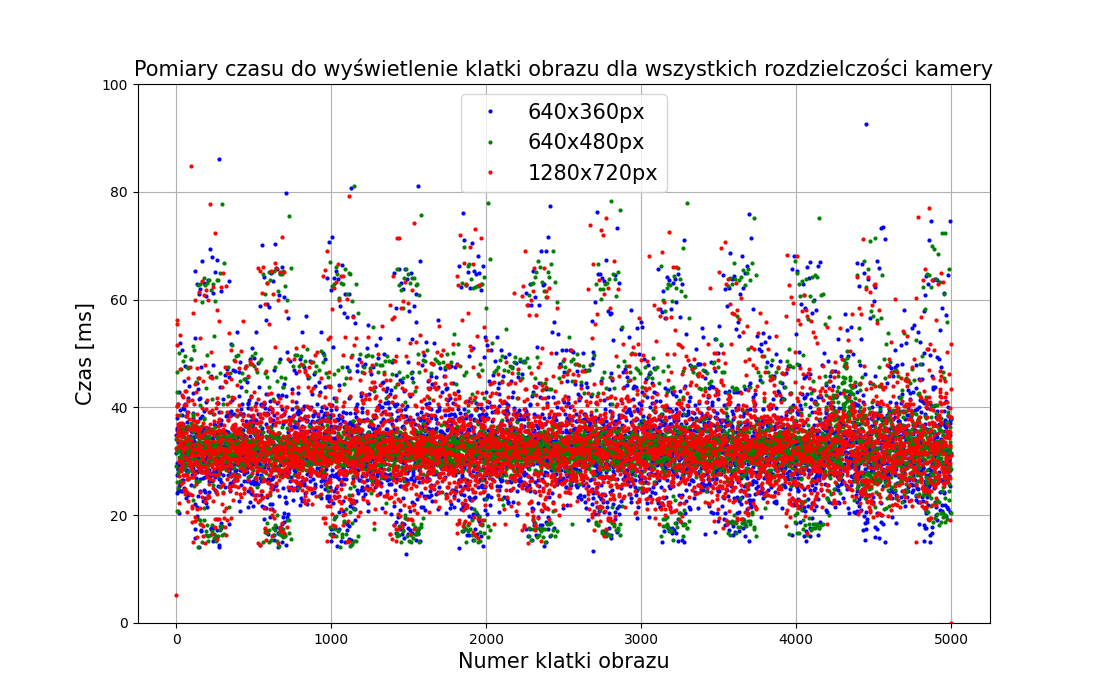
\includegraphics[width=\linewidth]{r_test_szybkosci/punkty/all.png}
    \caption{Wykres punktowy dla wszystich rozdzielczości przedstawiający pomiary czasu do wyświetlenia obrazu dla każdej klatki.}
    \label{fig:czas-punktowy-all}    
\end{figure}

Dla wyników dla każdej rozdzielczości można zaobserwować zagęsczenie punktów przy średniej wartości. 
Zagęsczenie pomiędzy rozdzielczościami można ocenić na podobne, chociaż na korzyść wyróżnia się rozdzielczośc 640x480px. Może być to spowodowane tym, że jest to ustawienie najbliżej odpowiadające użytemu, domyślnemu rozmiarowi obrazu poddanemu detekcji w YOLOv8n, które wynosi 640x640px. Wpływ mogły mieć również czynniki zewnętrzene takie jak mniejsze zajęcia procesora przez inne programy działające w komputerze.  

Zagęszczenie pokazuje pewien stopień powtarzalności. Mimo to na tym etapie testów system nie można uznać za powtarzalny. Liczba przetestowanych klatek nie pozwala wizualnie ocenić charakterystyki odchyleń od średniej. W celu dalszych testów możnaby możnaby parokrotnie zbadać mniejszą liczbe klatek i sprawdzić czy odchylenia mają naturę całkowicie losową albo czy występuje pewna zależność np. wystąpienie pewnego podzbioru, dla którego odchylenia najpierw rosną, a później maleją. Wykonanie takiego badania nie jest natomiast w pełni konieczne. Priorytetem systemu jest alarmowanie użytkownika z możliwie jak najmniejszym opóźniem, co eliminuje konieczność utrzymania stałego czasu wykonania. Biorąc to pod uwagę badaniu poddanoby tylko odchylenia większe od średniej. 

Sam fakt wystąpienia odchyleń nie definiuje jak bardzo opóźnione są alarmy wysyłane przez system. Wykresy pokazały, że nawet w sytuacji wystąpienia odchylenia, wyniki dla kolejnych klatek dalej są w większości zagęszczone w okolicy średniej i ponadto nie wystąpiła uznana za znaczącą zmiana w stopniu zagęsczenia. Dodatkowo wykres na ryskunku \ref{fig:czas-punktowy-all} pokazał również, iż zakres odchyleń można zaklasyfikować do tego samego zbioru dla wszystkich rozdzielczości.   
Podczas wykorzystania systemu jako użytkownik jakościowo stwierdzono, iż opóźnienia w alarmowaniu są niezauważalne. 

Podsumowując, dla wykorzystanego wyposażenia sprzętowego, wykazano niezależność wyników od ustawionej rozdzielczości kamery. Ponadto stwierdzono, iż opóźnienia systemu z wynikających odchyleń od średniej nie wpływają na komfort użytkowania.


\chapter{Badania skuteczności detekcji obiektów YOLOv8n}
\label{chap:badania-skutecznosci}
Rozdział ten opisuje autorskie testy dokładności detekcji obiektów w zależności od różnych, dobranych poziomów oświetlenia w nagrywanym pomieszczeniu oraz różnych wartości parametru progu ufności (opisanego w rozdziale \ref{chap:wprowadzenie-yolo_interjes}) modelu YOLOv8. Testowanym zadaniem jest dokładność klasyfikacji obiektów. Nie zaimplementowano testów dokładności dla lokalizacji przestrzennej, ponieważ nie jest ona priorytetem w niniejszym systemie. Uznano, iż jakościowe stwierdzenie możliwości lokalizacji w fazie tworzenia systemu jest wystarczające, a rezultat uznano za zadowalający. 

Zaimplementowane dwa testy skuteczności klasyfikacji to:
\begin{enumerate}
    \item Test dokładności pojedyńczej klasy na przykładzie klasy \emph{człowiek} (ang. \emph{person}). 
    \item  Test poziomu generalizacji modelu dla różnych wariantów obiektu wchodzących w skład tej samej klasy. Analiza przeprowadzona na przykładzie klasy \emph{krzesło} (ang. \emph{chair}) i użytych wariantów: krzesło kuchenne, krzesło gamingowe (dalej nazywane fotelem). 
\end{enumerate}
W obu testech detektor był skonfigurowany, aby zwracać tylko wyniki zawierające obiekty klas \emph{człowiek} i \emph{krzesło}. Ponadto, każdy test używa filmów z tego samego zbioru nagrań. Dla każdego nagrania wygenerowano pewne metryki postawowe, które są wykorzystywane do analizy oraz wyznaczania kolejnych metryk już w konkretnym teście. Każda metryka została wygenerowana dla każdej wartości progu ufności objętej testem. Wartość progu zaczynają się od $0.00$, aby następnie rosnąć co interwał $0.01$, aż do maksymalnej wartości $1.00$. Daje to łącznie sto jeden sprawdzonych wartości. Generacje metryk podstawowych zaprogramowano jako test odizolowanego detektora od reszty systemu, ze względu na łatwość i czytelność implementacyjną oraz brak zależności dokładności detekcji od czynników systemowych (w przeciwnieśtwie do szybkośći).  

Biorąc pod uwagę tę strukturę, rodział ten wpierw porusza kwestie współdzielone przez oba testy (opis źródła wideo oraz metryk podstawowych) w sekcji \ref{sec:test-wspoldzielony}, a następnie omawia dalszą analize w sekcjach \ref{sec:test-1} i \ref{sec:test-2}.
 
Uwaga dotycząca zamieszconych rysunków: w rysunkach przedstawiających człowieka twarz została zamazana.


\section{Przygotowanie danych do testów}
\label{sec:test-wspoldzielony}
\subsection{Żródło wideo}
\label{sec:zrodlo_wideo}
Źródło wideo to nagrane w domowych warunkach, autorskie, krótkie filmy. Filmy nagrano na kamerze o rozdzielczości 640x480 pikseli. Obiektyw kamery jest statycznie usytuowany w tej samej lokalizacji dla każdego filmu i skierowany na wejście do pomieszczenia, w którym znajduje się kamera. Wygląd pomieszczenia przedstawiono na rysunku \ref{fig:test-dokladnosc-scena}.

\begin{figure}[H]
    \centering
    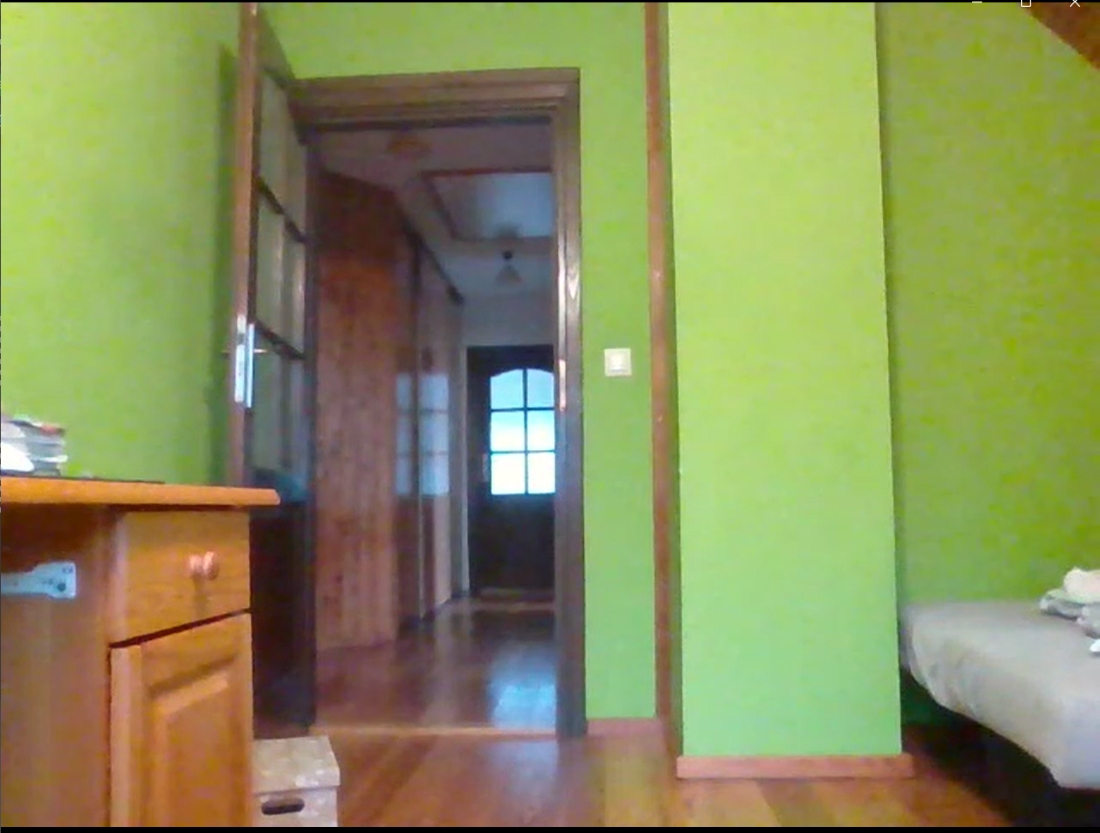
\includegraphics[width=\linewidth]{r_test_dokładności/vid_pics/1_1.jpg}
    \caption{Pomieszczenie, w którym nagrano filmy.}
    \label{fig:test-dokladnosc-scena}
\end{figure}

\begin{figure}[H]
    \centering
    \begin{minipage}{0.32\textwidth}
        \centering
        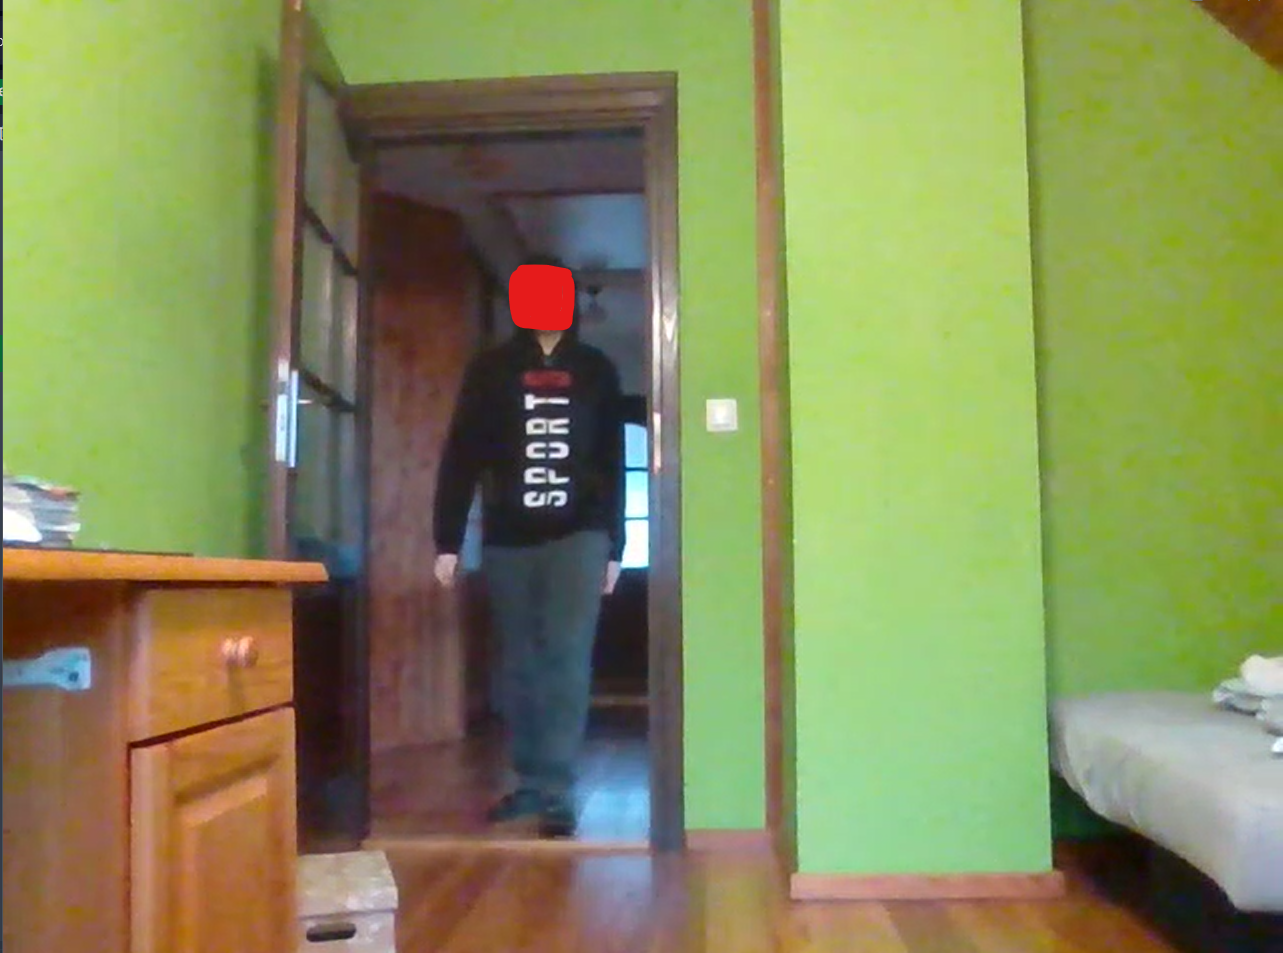
\includegraphics[width=\linewidth]{r_test_dokładności/vid_pics/1_2.png}
        \caption{Klatka filmu z człowiekiem.}
    \end{minipage}\hfill
    \begin{minipage}{0.32\textwidth}
        \centering
        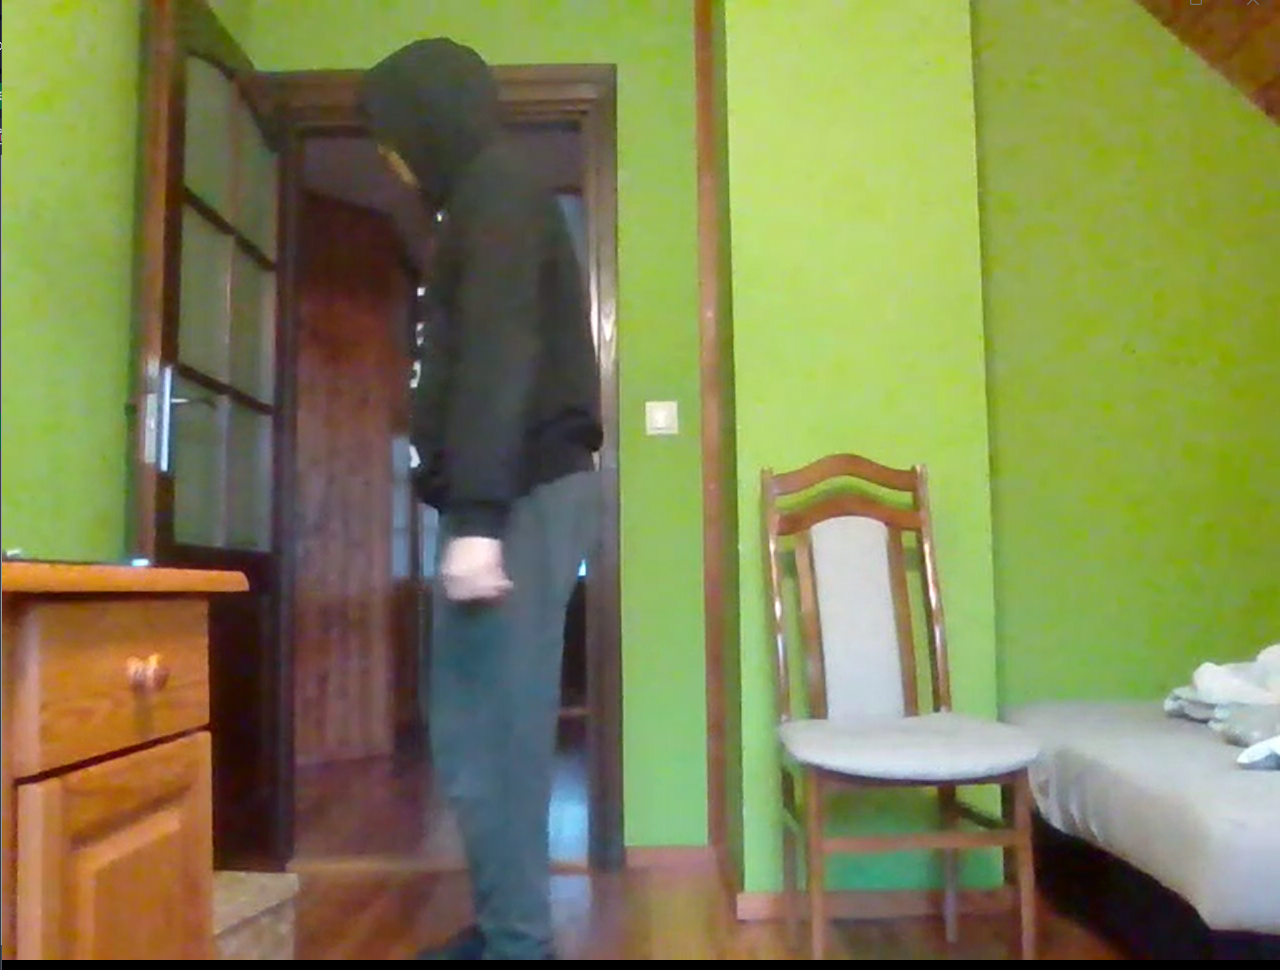
\includegraphics[width=\linewidth]{r_test_dokładności/vid_pics/1c_2.png}
        \caption{Klatka filmu z człowiekiem i krzesłem.}
    \end{minipage}\hfill
    \begin{minipage}{0.32\textwidth}
        \centering
        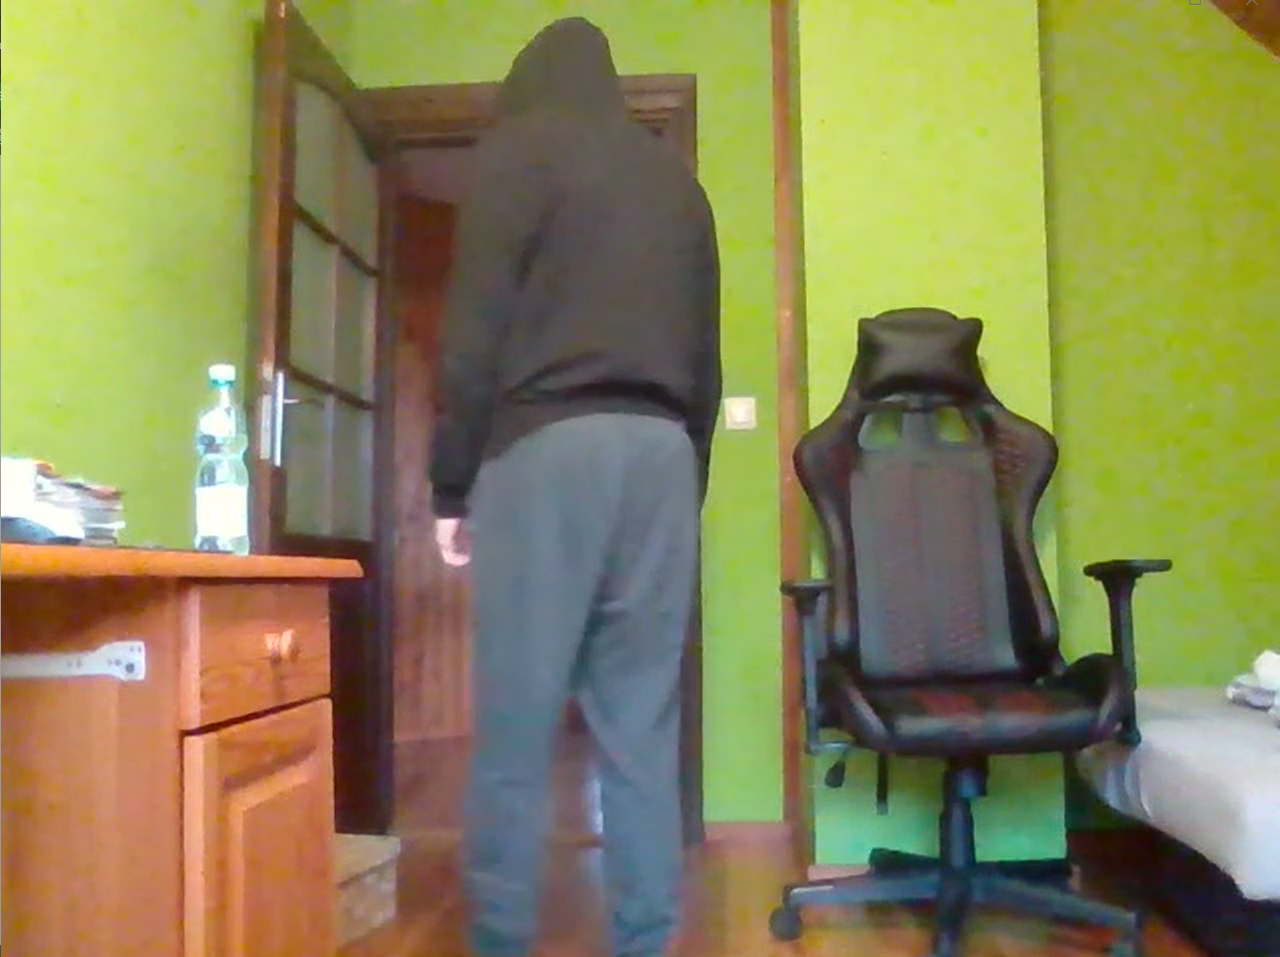
\includegraphics[width=\linewidth]{r_test_dokładności/vid_pics/1g_2.png}
        \caption{Klatka filmu z człowiekiem i fotelem.}
    \end{minipage}
    \caption{Prezentacja użytych obiektów.}
    \label{fig:all_objects}
\end{figure}
Filmy można podzielić na trzy kategorie ze względu na różne obecne w nim obiekty (wizualizacja objektów: rysunek \ref{fig:all_objects}):
\begin{itemize}
    \item człowiek
    \item człowiek, krzesło
    \item człowiek, fotel
\end{itemize}
Krzesło oraz fotel, z perspektywy filmów, są obiektami statycznymi. Przez całą długość filmu są umieszczone w jednej lokalizacji, a inne obiekty nie wchodzą z nimi w fizyczną interakcję.
Natomiast człowiek jest obiektem ruchomym. Jest on nieobecny przez pierwszą część każdego filmu. W drugiej części przekracza próg pomieszczenia, zbliża się do pewnego punktu widocznego w obiektywie, a pod koniec filmu wykonuje jeden pełen obrót wokół własnej osi. 

Należy podkreślić kilka istotnych kwestii dotyczących nagranych filmów:
\begin{itemize}
    \item Obecne obiekty nie wchodzą ze sobą w interakcję --- człowiek podczas ruchu nie zasłania konturów krzesła ani fotela.
    \item Generacja danych do testów nie odbywała się na każdej klatce nagranego filmu. Użyto tylko klatek, na których widoczne są pełne kontury obiektów. Pełny kontur człowieka pojawia się w momencie przekroczenia progu wejścia do pomieszczenia. W związku z powyższym, wykorzystano dwie sekcje każdego filmu: sekcję, w której człowiek był całkowicie nieobecny oraz sekcję od momentu przekroczenia progu.
\end{itemize}

Dla każdej kategorii filmu nagrano cztery warianty z różnym poziomem oświetlenia w pomieszczeniu, co daje łącznie dwanaście plików wideo do analizy. Wizualne różnice między poziomami przedstawiono na rysunku \ref{fig:person_grid} (człowiek), rysunku \ref{fig:chair_grid} (człowiek, krzesło) oraz rysunku \ref{fig:game_grid} (człowiek, fotel). 
Dla każdego filmu, korzystając z modelu przestrzeni barw HSV, obliczono średnią jasność oraz nasycenie. Wartości te zaprezentowano w tabeli \ref{tab:saturation-value-table}. Obliczenia polegały na wyznaczeniu średniej wartości jasności i nasycenia dla każdej klatki obrazu na podstawie wszystkich pikseli. Następnie wyznaczono średnią z uzyskanych wartości dla wszystkich klatek w filmie.
\begin{table}[H]
    \centering
    \caption{Jasność i nasycenie dla każdego nagranego filmu.}
    \begin{tabular}{|c|c|c|c|}
    \hline
    Nr sceny:          & Obecne obiekty    & Jasność & Nasycenie \\ \hline
    \multirow{3}{*}{1} & człowiek          & 152.73  & 107.3     \\ \cline{2-4} 
                       & człowiek, krzesło & 149.92  & 119.07    \\ \cline{2-4} 
                       & człowiek, fotel   & 152.68  & 111.47    \\ \hline
    \multirow{3}{*}{2} & człowiek          & 134.64  & 93.48     \\ \cline{2-4} 
                       & człowiek, krzesło & 139.14  & 90.71     \\ \cline{2-4} 
                       & człowiek, fotel   & 133.77  & 83.29     \\ \hline
    \multirow{3}{*}{3} & człowiek          & 41.59   & 123.48    \\ \cline{2-4} 
                       & człowiek, krzesło & 38.91   & 132.31    \\ \cline{2-4} 
                       & człowiek, fotel   & 38.12   & 124.31    \\ \hline
    \multirow{3}{*}{4} & człowiek          & 25.47   & 90.92     \\ \cline{2-4} 
                       & człowiek, krzesło & 25.3    & 100.8     \\ \cline{2-4} 
                       & człowiek, fotel   & 24.88   & 108.5     \\ \hline
    \end{tabular}
    \label{tab:saturation-value-table}
    \end{table}
\begin{figure}[H]
    \centering
    \begin{minipage}{0.45\textwidth}
        \centering
        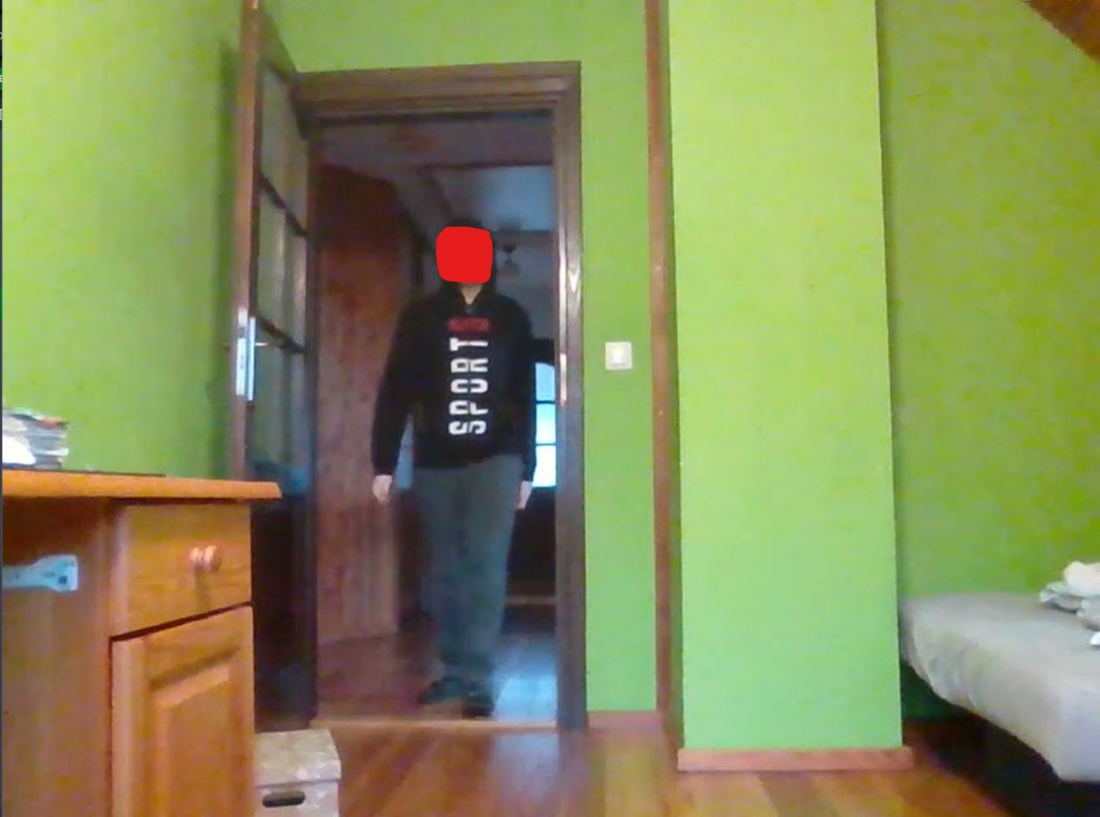
\includegraphics[width=\linewidth]{r_test_dokładności/vid_pics/1_2.jpg}
    \end{minipage}\hfill
    \begin{minipage}{0.45\textwidth}
        \centering
        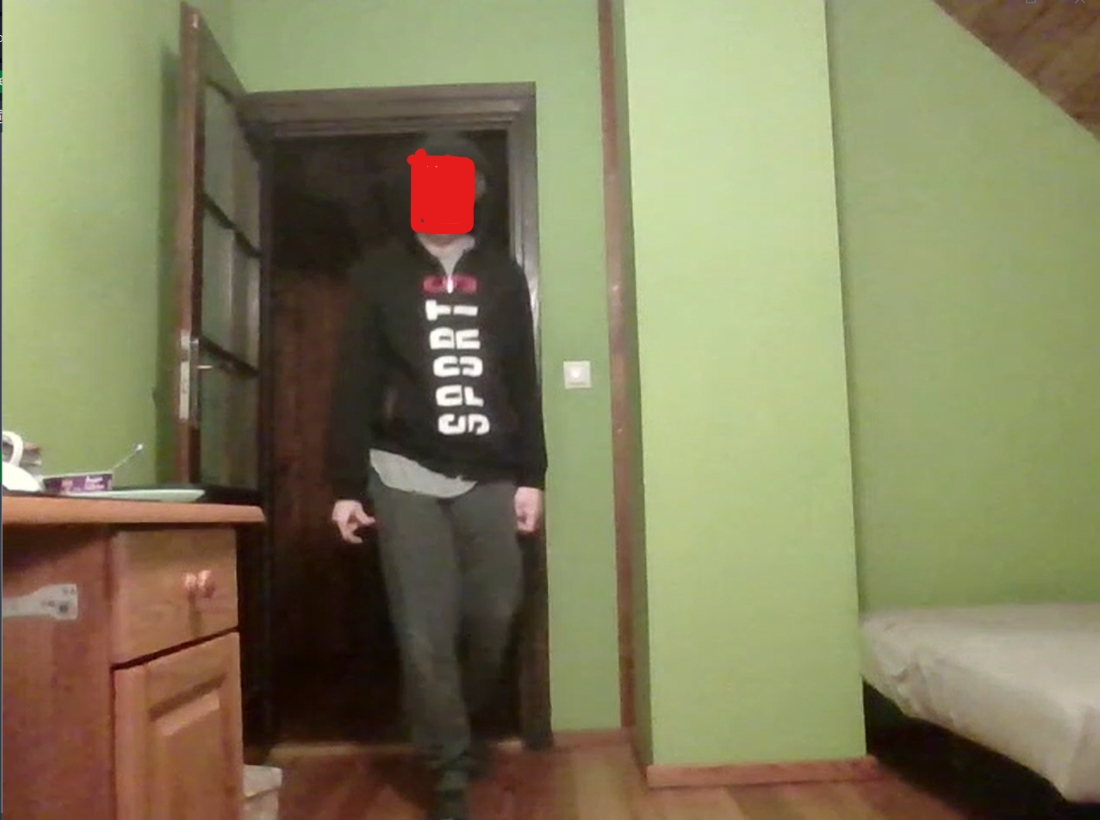
\includegraphics[width=\linewidth]{r_test_dokładności/vid_pics/2_2.jpg}
    \end{minipage}
    \vskip\baselineskip
    \begin{minipage}{0.45\textwidth}
        \centering
        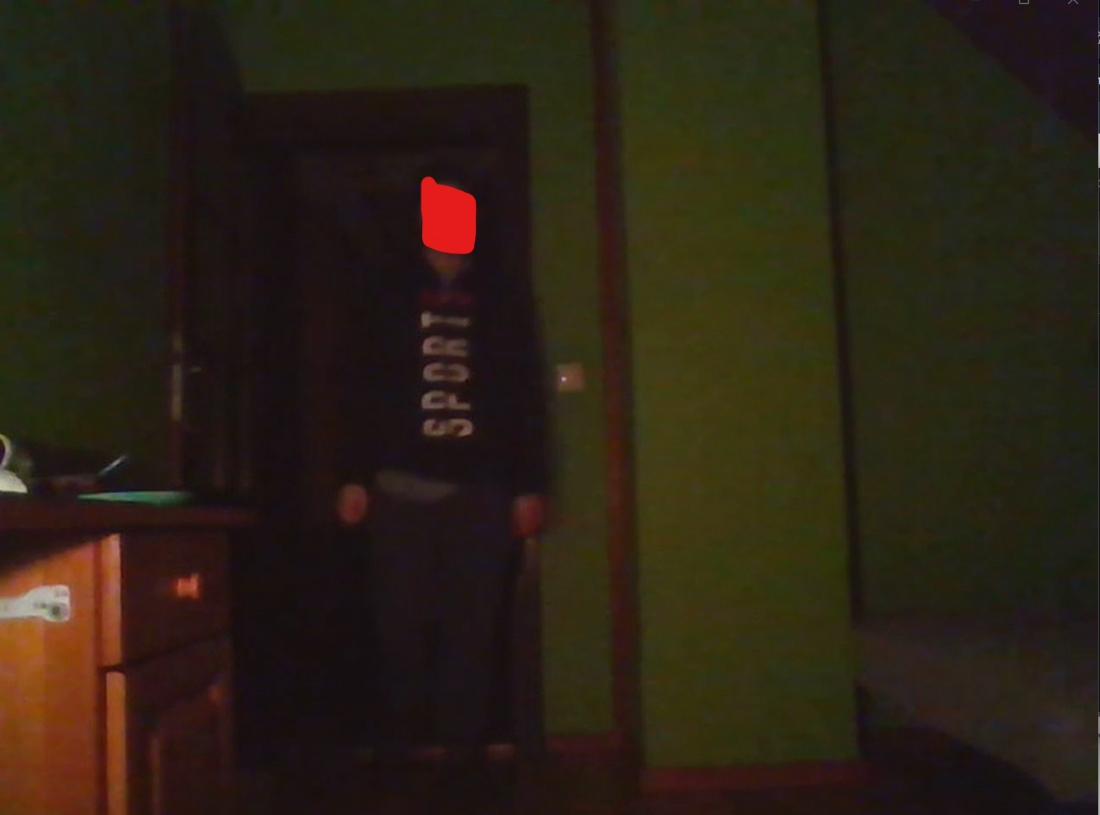
\includegraphics[width=\linewidth]{r_test_dokładności/vid_pics/3_2.jpg}
    \end{minipage}\hfill
    \begin{minipage}{0.45\textwidth}
        \centering
        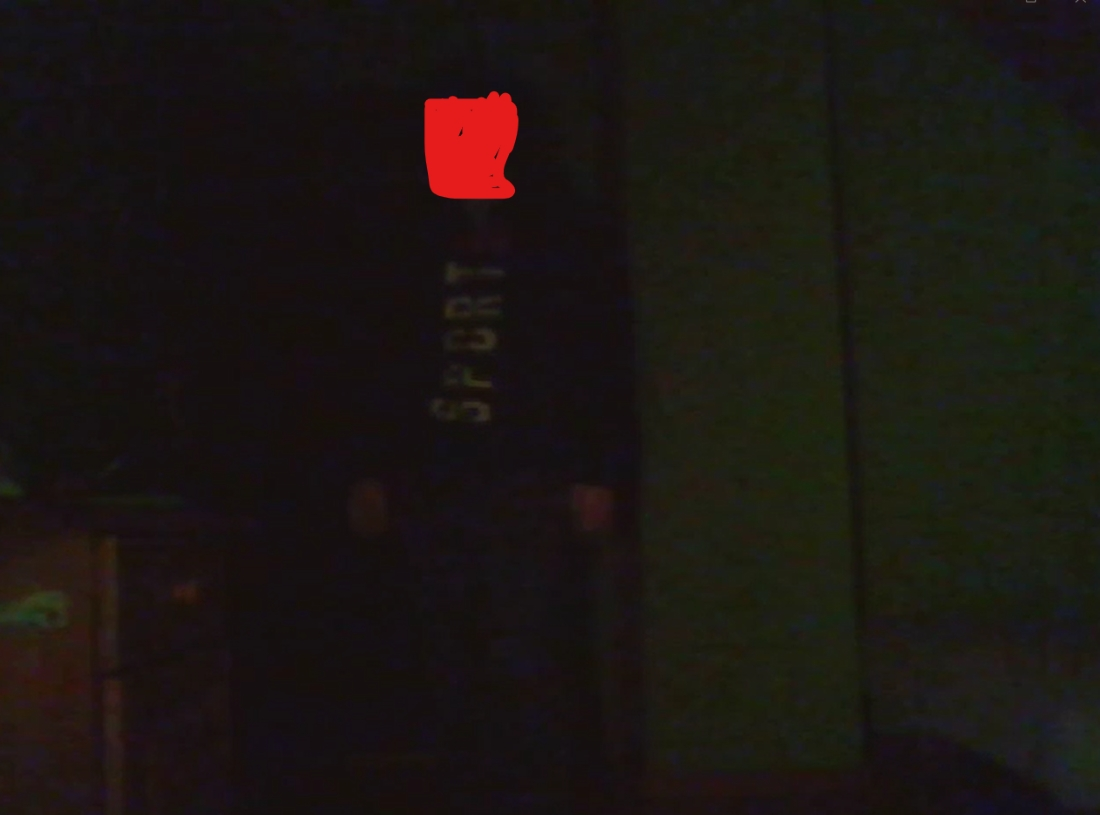
\includegraphics[width=\linewidth]{r_test_dokładności/vid_pics/4_2.jpg}
    \end{minipage}
    \caption{Poziomy oświetlenia dla filmów z obecnym człowiekiem}
    \label{fig:person_grid}
\end{figure}
\begin{figure}[H]
    \centering
    \begin{minipage}{0.45\textwidth}
        \centering
        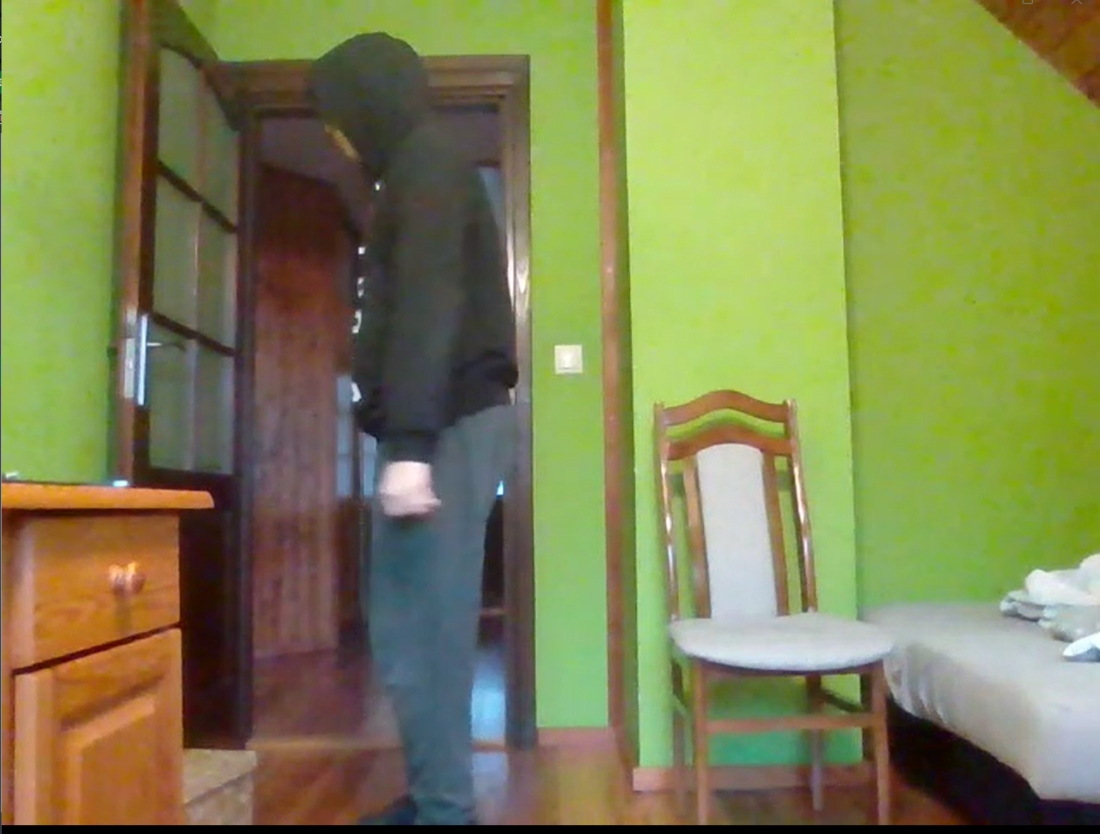
\includegraphics[width=\linewidth]{r_test_dokładności/vid_pics/1c_2.jpg}
    \end{minipage}\hfill
    \begin{minipage}{0.45\textwidth}
        \centering
        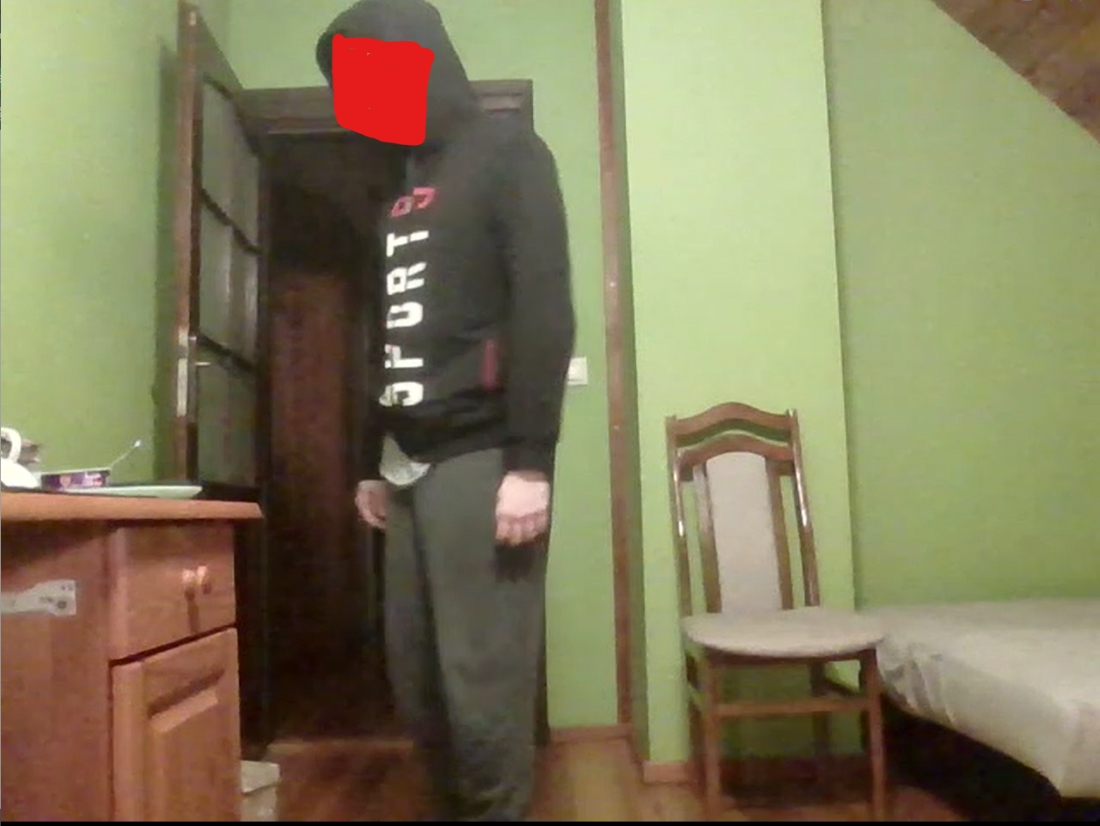
\includegraphics[width=\linewidth]{r_test_dokładności/vid_pics/2c_2.jpg}
    \end{minipage}
    \vskip\baselineskip
    \begin{minipage}{0.45\textwidth}
        \centering
        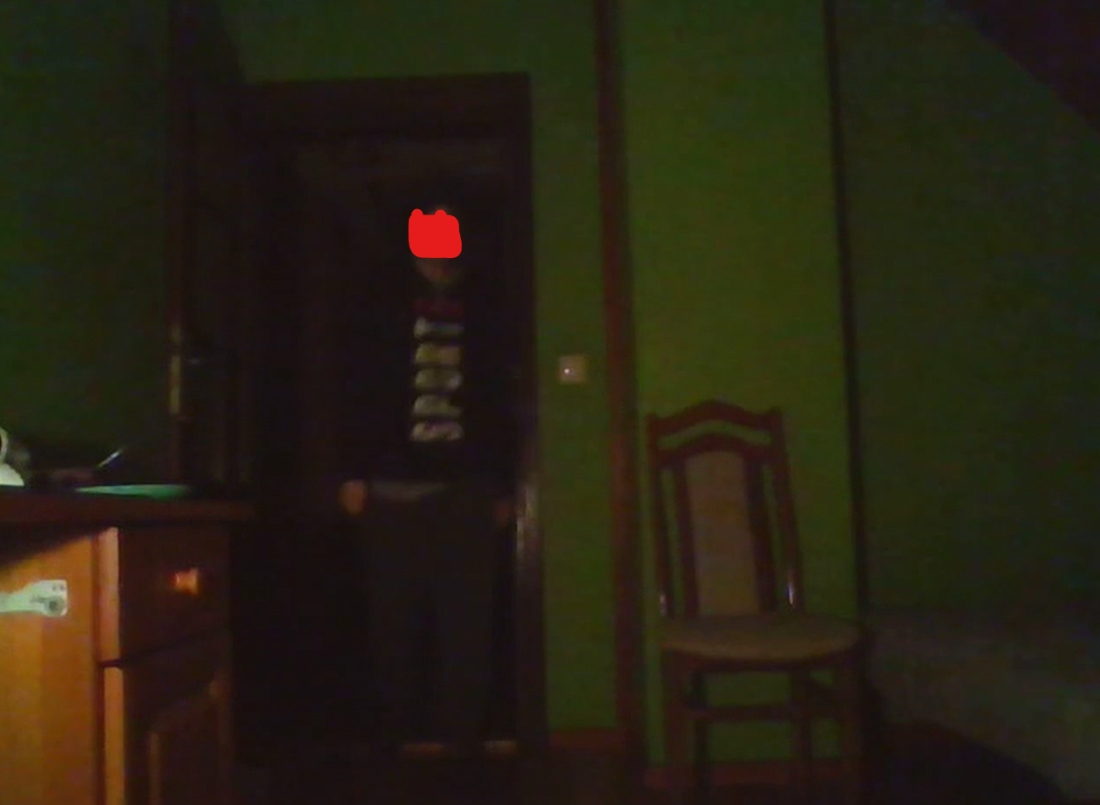
\includegraphics[width=\linewidth]{r_test_dokładności/vid_pics/3c_2.jpg}
    \end{minipage}\hfill
    \begin{minipage}{0.45\textwidth}
        \centering
        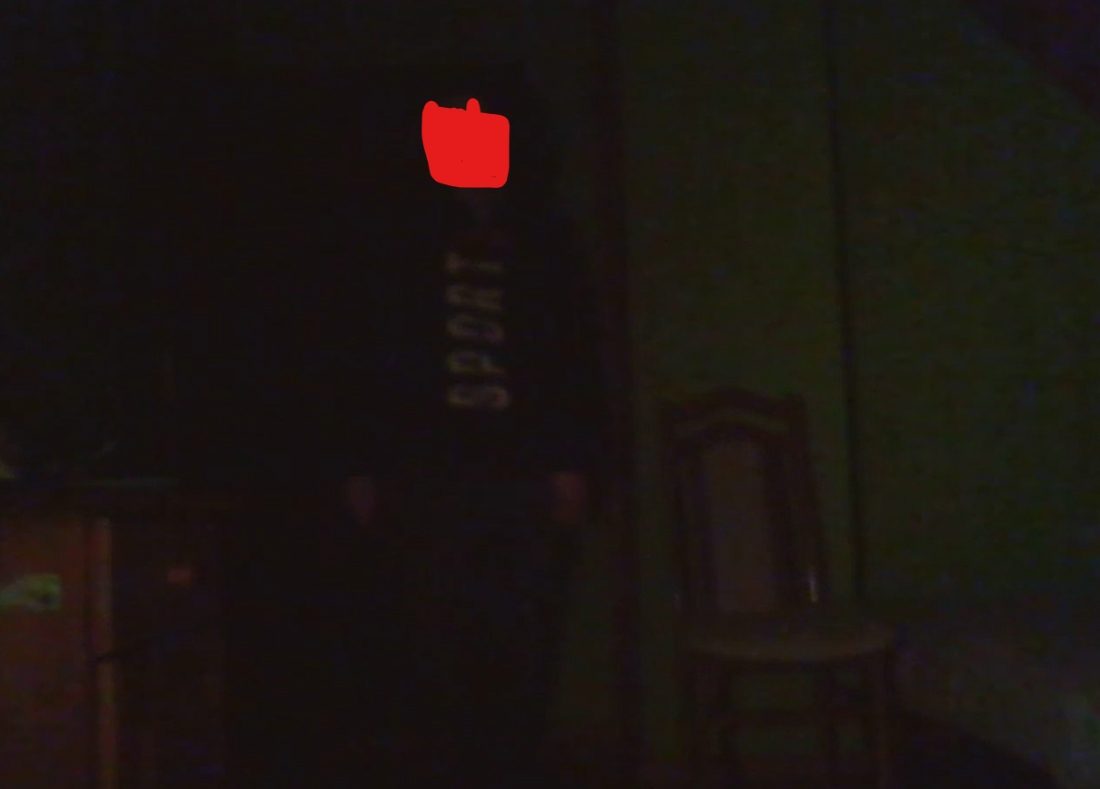
\includegraphics[width=\linewidth]{r_test_dokładności/vid_pics/4c_2.jpg}
    \end{minipage}
    \caption{Poziomy oświetlenia dla filmów z obecnym człowiekiem i krzesłem}
    \label{fig:chair_grid}
\end{figure}
\begin{figure}[H]
    \centering
    \begin{minipage}{0.45\textwidth}
        \centering
        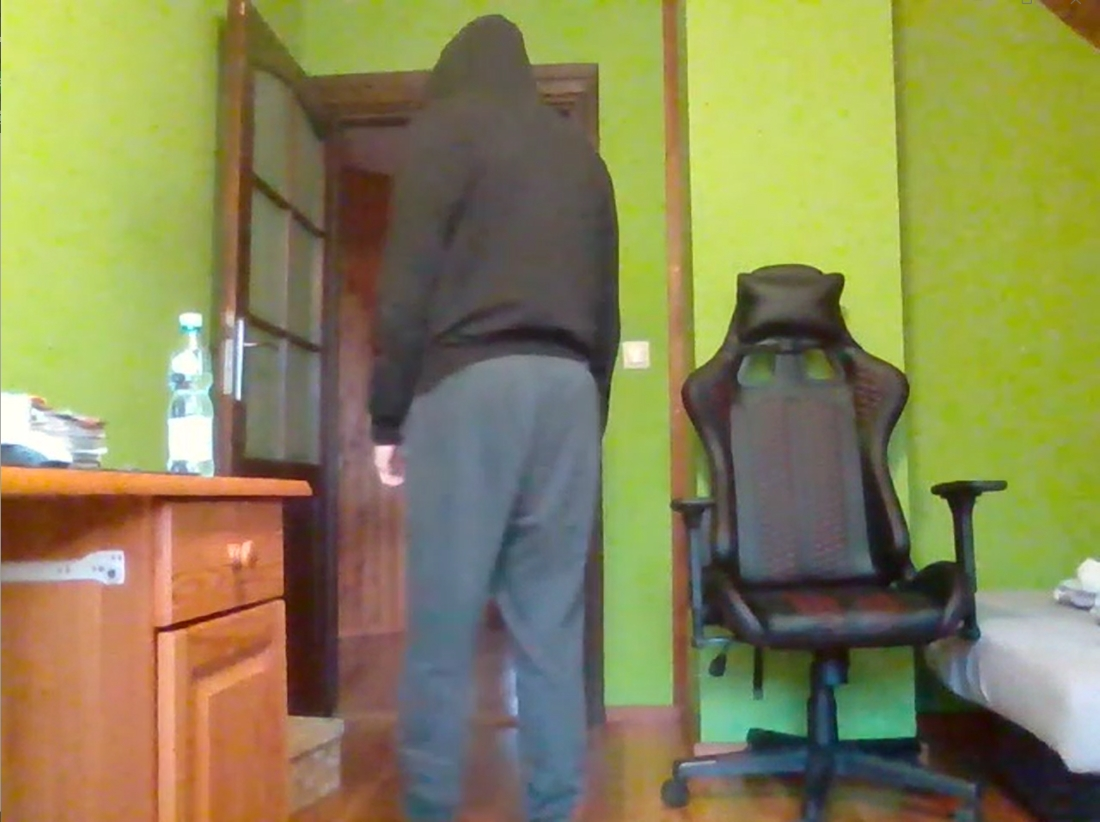
\includegraphics[width=\linewidth]{r_test_dokładności/vid_pics/1g_2.jpg}
    \end{minipage}\hfill
    \begin{minipage}{0.45\textwidth}
        \centering
        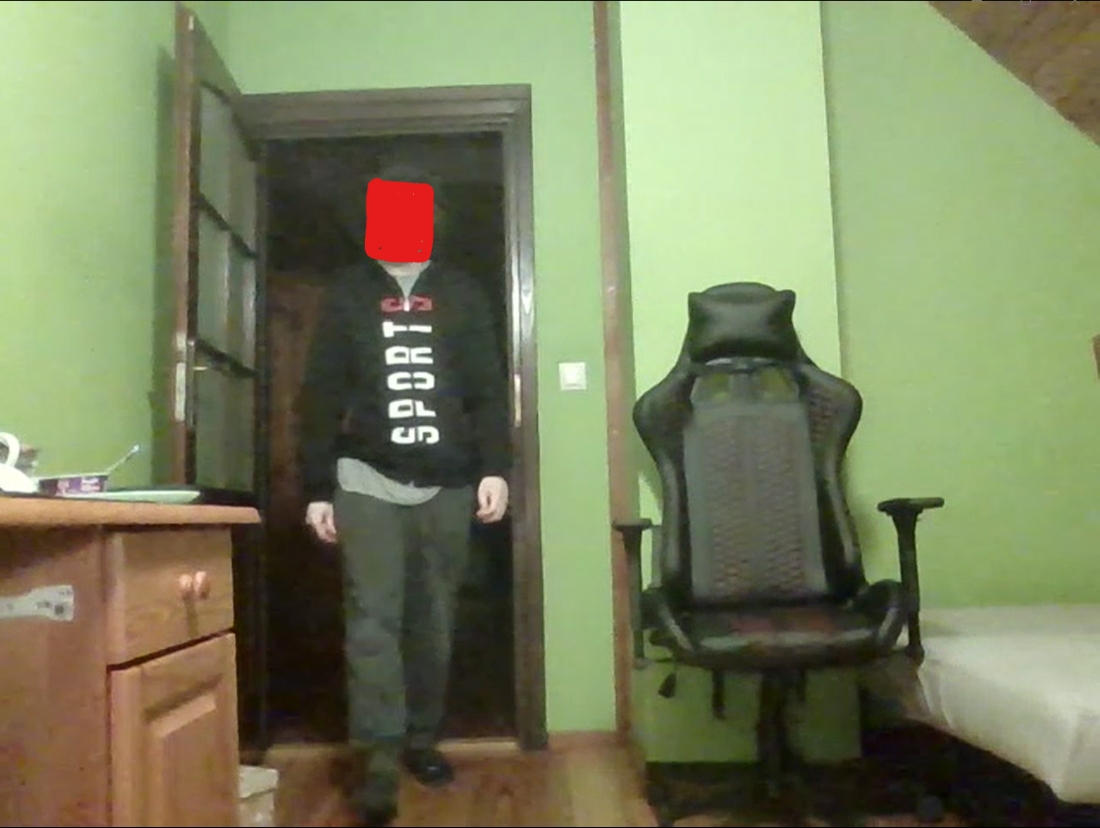
\includegraphics[width=\linewidth]{r_test_dokładności/vid_pics/2g_2.jpg}
    \end{minipage}
    \vskip\baselineskip
    \begin{minipage}{0.45\textwidth}
        \centering
        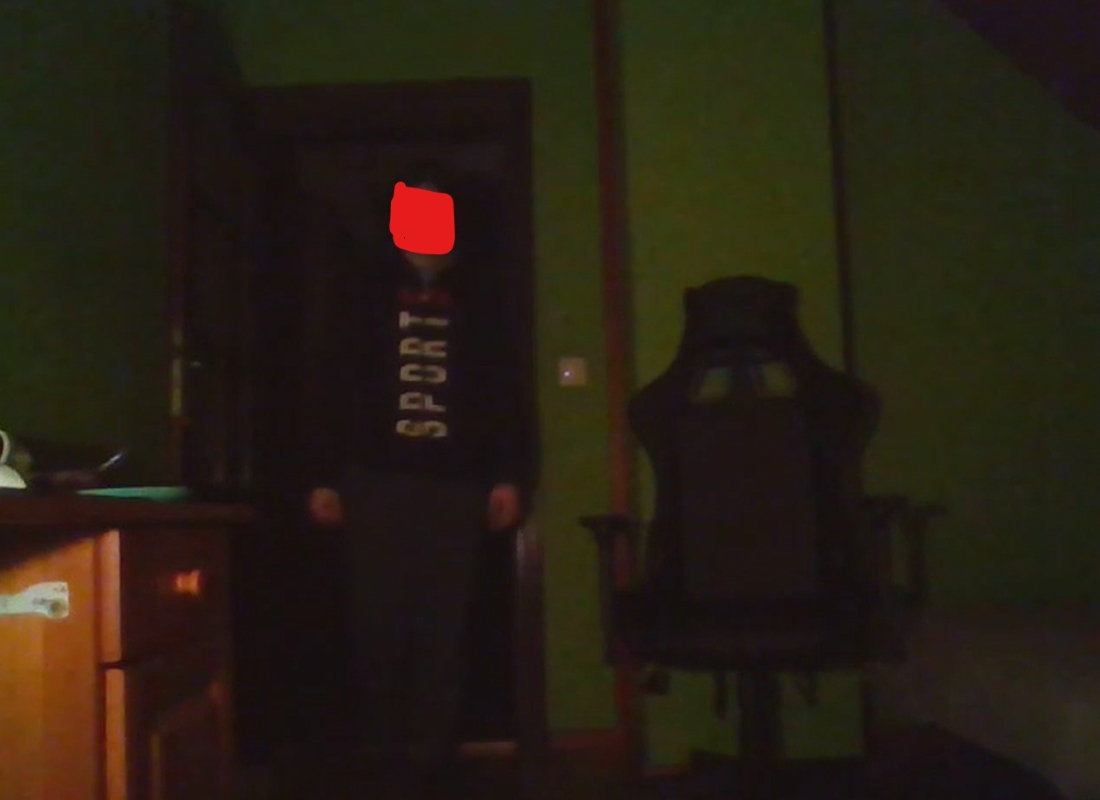
\includegraphics[width=\linewidth]{r_test_dokładności/vid_pics/3g_2.jpg}
    \end{minipage}\hfill
    \begin{minipage}{0.45\textwidth}
        \centering
        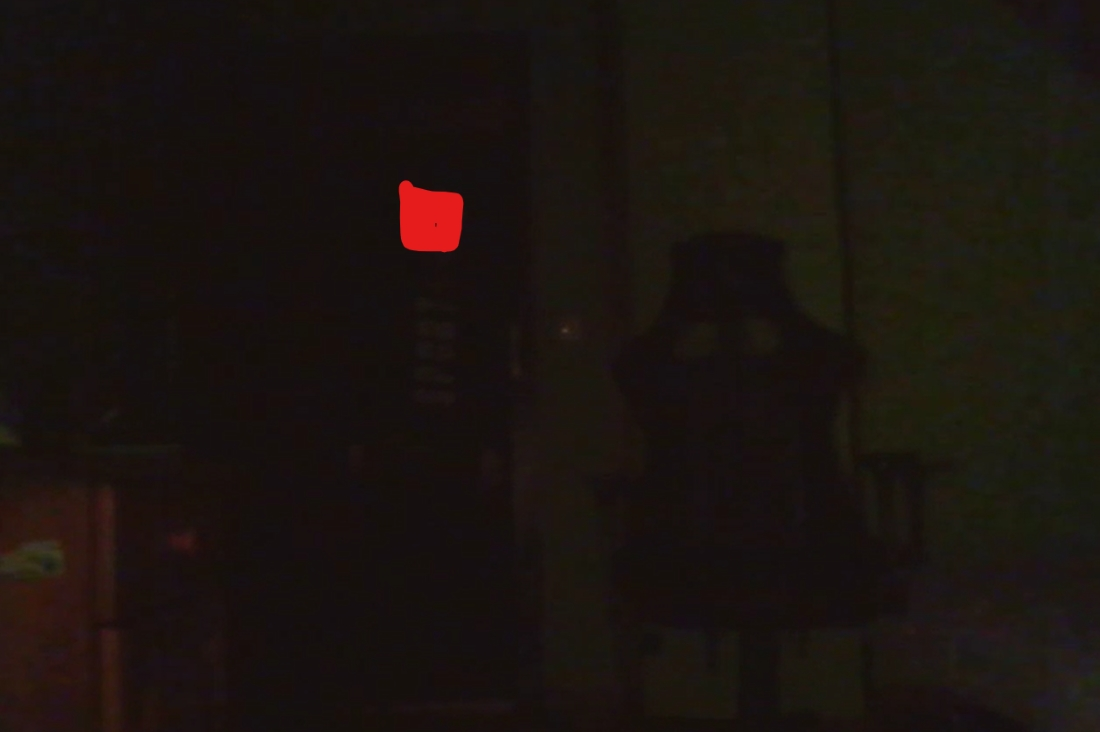
\includegraphics[width=\linewidth]{r_test_dokładności/vid_pics/4g_2.jpg}
    \end{minipage}
    \caption{Poziomy oświetlenia dla filmów z obecnym człowiekiem i fotelem}
    \label{fig:game_grid}
\end{figure}







\subsection{Metryki i dane wynikowe używane w testach}
Na podstawie opisanych dwunastu plików wideo wygenerowano dane do analizy w testach dla każdego z nich. Dane te to podstawowe metryki używane w klasyfikacji binarnej. Są to: wynik prawdziwy pozytywny (TP), wynik prawdziwy negatywny (TN), wynik fałszywy pozytywny (FP), wynik fałszywy negatywny (FN). 
Zaprojektowane testy sprawdzają tylko jedną klasę na test --- np. dla ewaluacji klasyfikacji klasy \emph{człowiek}, ignorowane są wykrycia innych klas. Co więcej, w niniejszym systemie nacisk kładziony jest na alarmowanie użytkownika o obecności obiektu, dlatego też uznano, iż więcej niż jedna detekcja klasy będzie przypisana do tej samej metryki co detekcja pojedynczego obiektu. 

Biorąc to pod uwagę, definicję metryk skonstruowano następująco: \\ \\ \noindent
Znaczenie skrótów z tabeli \ref{tab:saturation-value-table}: \\
$\emptyset$ -- brak wystąpienia obiektu wykrywanej klasy \\
x -- pojedyncze wystąpienie obiektu wykrywanej klasy \\
n*x -- wielokrotne wystąpienie obiektu wykrywanej klasy
\begin{table}[H]
    \centering
    \caption{Definicja metryk generowanych podczas testów detekcji obiektów.}
    \begin{tabular}{|>{\centering\arraybackslash}m{2cm}|>{\centering\arraybackslash}m{2cm}|>{\centering\arraybackslash}m{2.5cm}|>{\raggedright\arraybackslash}m{7.5cm}|}
    \hline
    Metryka & Obiekty na nagraniu & Obiekty wykryte przez detektor & \multicolumn{1}{c|}{Opis} \\ \hline



    \multirow{2}{*}{TP} & \multirow{2}{*}{x} & x & \multirow{2}{7.5cm}{Detektor wykrył jeden lub więcej obiektów klasy x, gdy obiekt x był obecny.} \\ \cline{3-3}

     &  & n*x & \\ \cline{1-4}



    TN & $\emptyset$ & $\emptyset$ & Detektor nie wykrył ani jednego obiektu klasy x, gdy obiekt x był nieobecny. \\ \hline

    

    \multirow{2}{*}{TN} & \multirow{2}{*}{$\emptyset$} & x & \multirow{2}{7.5cm}{Detektor wykrył jeden lub więcej obiektów klasy x, mimo że obiekt był nieobecny.} \\ \cline{3-3}

     &  & n*x & \\ \cline{1-4}



    FN & x & $\emptyset$ & Detektor nie wykrył ani jednego obiektu klasy x, mimo że obiekt był obecny. \\ \hline
    \end{tabular}
\end{table}

Generacja metryk wynikowych odbywa się w następująco:
\begin{enumerate}
    \item Wybierany jest film.
    \item Dla filmu metryki generowane są dla każdej badanej wartości progu ufności.
    \item Dla progu ufności analizowana jest każda klatka spełniająca wymagania opisane w rozdziale \ref{sec:zrodlo_wideo}. Dana klatka jest kategoryzowana do jednej z metryk.
    \item Metryka wynikowa to liczba klatek przypisanych do tej metryki.
\end{enumerate} 
Przykład wygenerowanych wyników prezentuje tabela \ref{tab:example-generated}.
\begin{table}[H]
    \centering
    \caption{Struktura wygenerowanych wyników na przykładzie częściowych wyników dla filmu z obecnym człowiekiem dla poziomu oświetlania nr 1. Wartości metryk to liczba klatek filmu przypisana do każdej z nich.}
    \begin{tabular}{ccccc}
    \hline
    \multicolumn{1}{|c|}{Próg   ufności} & \multicolumn{1}{c|}{TP}                    & \multicolumn{1}{c|}{TN}                    & \multicolumn{1}{c|}{FP}                    & \multicolumn{1}{c|}{FN}                    \\ \hline
    \multicolumn{1}{|c|}{0}                                 & \multicolumn{1}{c|}{100}                   & \multicolumn{1}{c|}{0}                     & \multicolumn{1}{c|}{122}                   & \multicolumn{1}{c|}{0}                     \\ \hline
    \multicolumn{1}{|c|}{0.01}                              & \multicolumn{1}{c|}{100}                   & \multicolumn{1}{c|}{49}                    & \multicolumn{1}{c|}{73}                    & \multicolumn{1}{c|}{0}                     \\ \hline
    \multicolumn{1}{|c|}{0.02}                              & \multicolumn{1}{c|}{100}                   & \multicolumn{1}{c|}{104}                   & \multicolumn{1}{c|}{18}                    & \multicolumn{1}{c|}{0}                     \\ \hline
    \multicolumn{1}{|c|}{0.03}                              & \multicolumn{1}{c|}{100}                   & \multicolumn{1}{c|}{120}                   & \multicolumn{1}{c|}{2}                     & \multicolumn{1}{c|}{0}                     \\ \hline
    \multicolumn{1}{|c|}{0.04}                              & \multicolumn{1}{c|}{100}                   & \multicolumn{1}{c|}{122}                   & \multicolumn{1}{c|}{0}                     & \multicolumn{1}{c|}{0}                     \\ \hline
    \multicolumn{5}{c}{$\bullet$ $\bullet$   $\bullet$ $\bullet$ $\bullet$ $\bullet$ $\bullet$ $\bullet$ $\bullet$   $\bullet$ $\bullet$ $\bullet$ $\bullet$ $\bullet$ $\bullet$ $\bullet$   $\bullet$ $\bullet$ $\bullet$ $\bullet$ $\bullet$} \\ \hline
    \multicolumn{1}{|c|}{0.96}                              & \multicolumn{1}{c|}{0}                     & \multicolumn{1}{c|}{122}                   & \multicolumn{1}{c|}{0}                     & \multicolumn{1}{c|}{100}                   \\ \hline
    \multicolumn{1}{|c|}{0.97}                              & \multicolumn{1}{c|}{0}                     & \multicolumn{1}{c|}{122}                   & \multicolumn{1}{c|}{0}                     & \multicolumn{1}{c|}{100}                   \\ \hline
    \multicolumn{1}{|c|}{0.98}                              & \multicolumn{1}{c|}{0}                     & \multicolumn{1}{c|}{122}                   & \multicolumn{1}{c|}{0}                     & \multicolumn{1}{c|}{100}                   \\ \hline
    \multicolumn{1}{|c|}{0.99}                              & \multicolumn{1}{c|}{0}                     & \multicolumn{1}{c|}{122}                   & \multicolumn{1}{c|}{0}                     & \multicolumn{1}{c|}{100}                   \\ \hline
    \multicolumn{1}{|c|}{1}                                 & \multicolumn{1}{c|}{0}                     & \multicolumn{1}{c|}{122}                   & \multicolumn{1}{c|}{0}                     & \multicolumn{1}{c|}{100}                   \\ \hline
    \end{tabular}
    \label{tab:example-generated}
    \end{table}


\section{Test dokładności pojedyńczej klasy}
\label{sec:test-1}
Niniejszy podrozdział przedstawia różne badania, których celem jest ewaluacja klasyfikacji YOLOv8n na przykładzie klasy człowiek. Model zbadano pod kątem wpływu jak manipulacja poziomem oświetlenia oraz progu ufności przekłada się na jego wyniki. Dla każdego zmierzonego progu ufności wyznaczane będą metryki potrzebne do zobrazowania wniosków. Będą one liczone na podstawie poprzednio uzyskanych metryk --- TP, TN, FP i FN. Do testu wykrzystano cztery filmy. Każdy z nich przedstawia wyłącznie człowieka. Wartości jasności i nasycenia przedstawiono w tabeli \ref{tab:saturacja-jasnosc-czlowiek}. Wygląd nagranego pomieszczenia dla różnych poziomów oświetlenia ukazano na rysunku \ref{fig:person_grid}. 

\begin{table}[H]
\centering
\caption{Jasność i nasycenie dla wszystkich filmów.}
\begin{tabular}{|c|c|c|c|}
\hline
Poziom oświetlenia  & Obecne obiekty & Jasność & Nasycenie \\ \hline
1        & człowiek       & 152.73  & 107.3     \\ \hline
2        & człowiek       & 134.64  & 93.48     \\ \hline
3        & człowiek       & 41.59   & 123.48    \\ \hline
4        & człowiek       & 25.47   & 90.92     \\ \hline
\end{tabular}

\label{tab:saturacja-jasnosc-czlowiek}
\end{table}


\subsection{Ewaluacja modelu dla różnych poziomów oświetlenia}
\label{sec:test-AUC}
W celu zobrazowania i oceniania wyniku modelu zastosowano metrykę 

\begin{figure}[H]
    \centering
    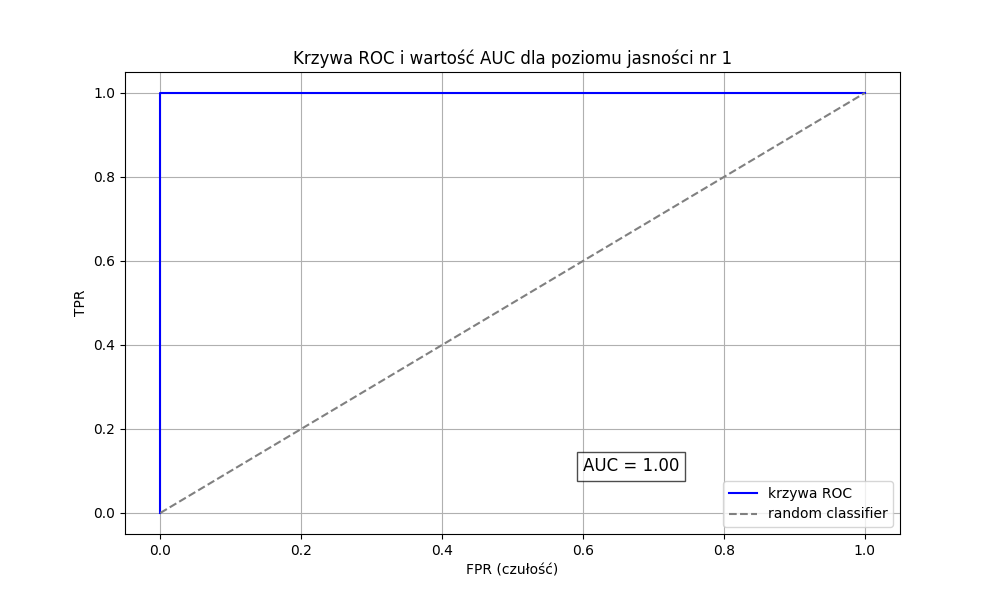
\includegraphics[width=\linewidth]{r_test_dokładności/AUC_charts/1.png}
    \caption{Krzywa ROC i wartość AUC dla poziomu jasności nr 1.}
    \label{fig:ROC-1}
\end{figure}

\begin{figure}[H]
    \centering
    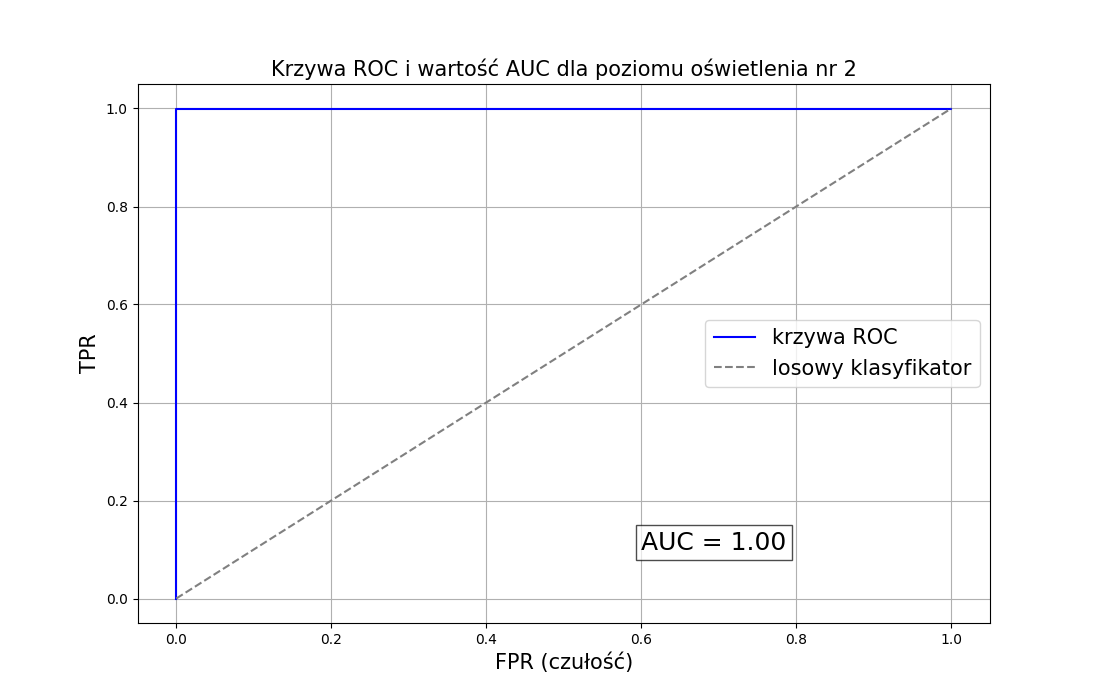
\includegraphics[width=\linewidth]{r_test_dokładności/AUC_charts/2.png}
    \caption{Krzywa ROC i wartość AUC dla poziomu jasności nr 2.}
    \label{fig:ROC-2}
\end{figure}

\begin{figure}[H]
    \centering
    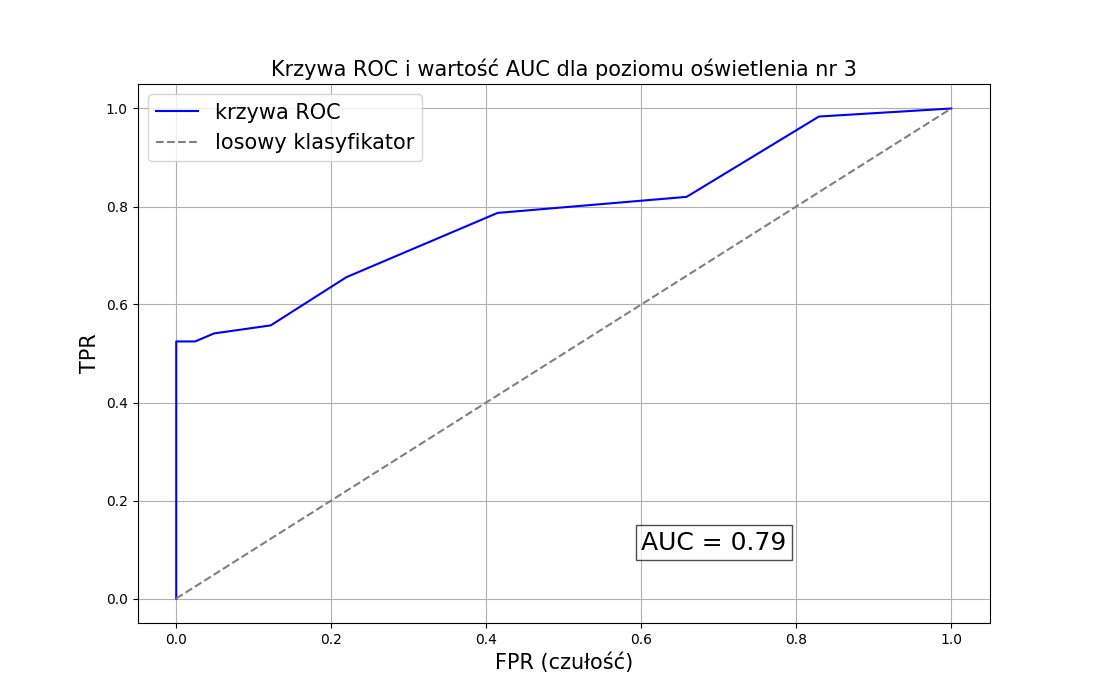
\includegraphics[width=\linewidth]{r_test_dokładności/AUC_charts/3.png}
    \caption{Krzywa ROC i wartość AUC dla poziomu jasności nr 3.}
    \label{fig:ROC-3}
\end{figure}

\begin{figure}[H]
    \centering
    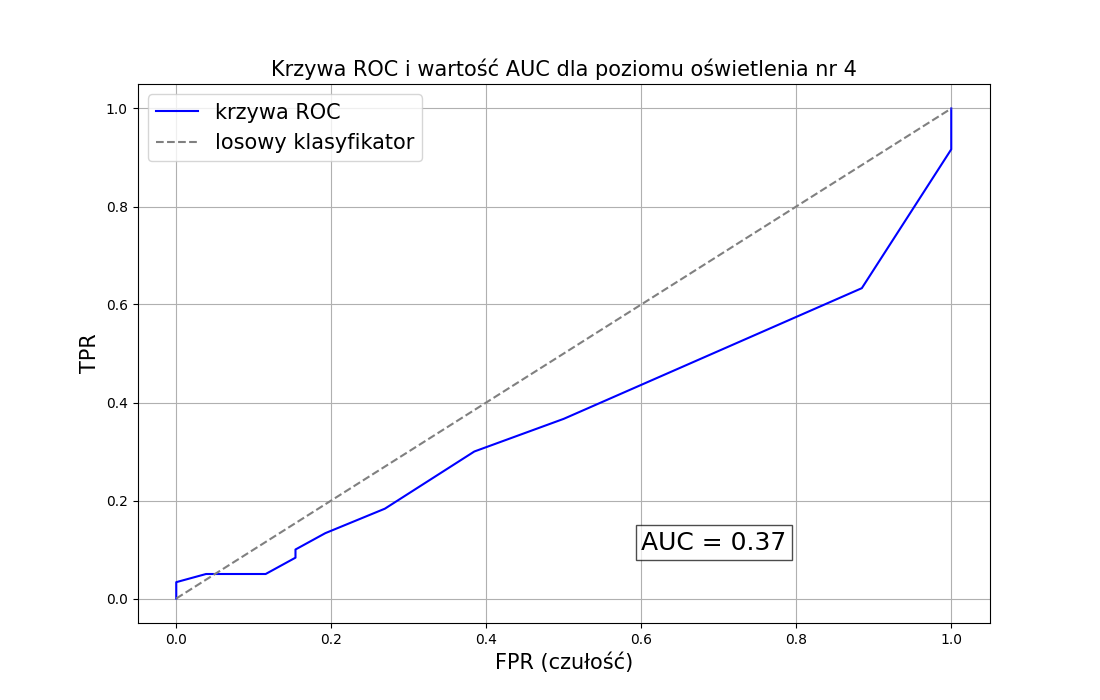
\includegraphics[width=\linewidth]{r_test_dokładności/AUC_charts/4.png}
    \caption{Krzywa ROC i wartość AUC dla poziomu jasności nr 4.}
    \label{fig:ROC-4}
\end{figure}

\begin{figure}[H]
    \centering
    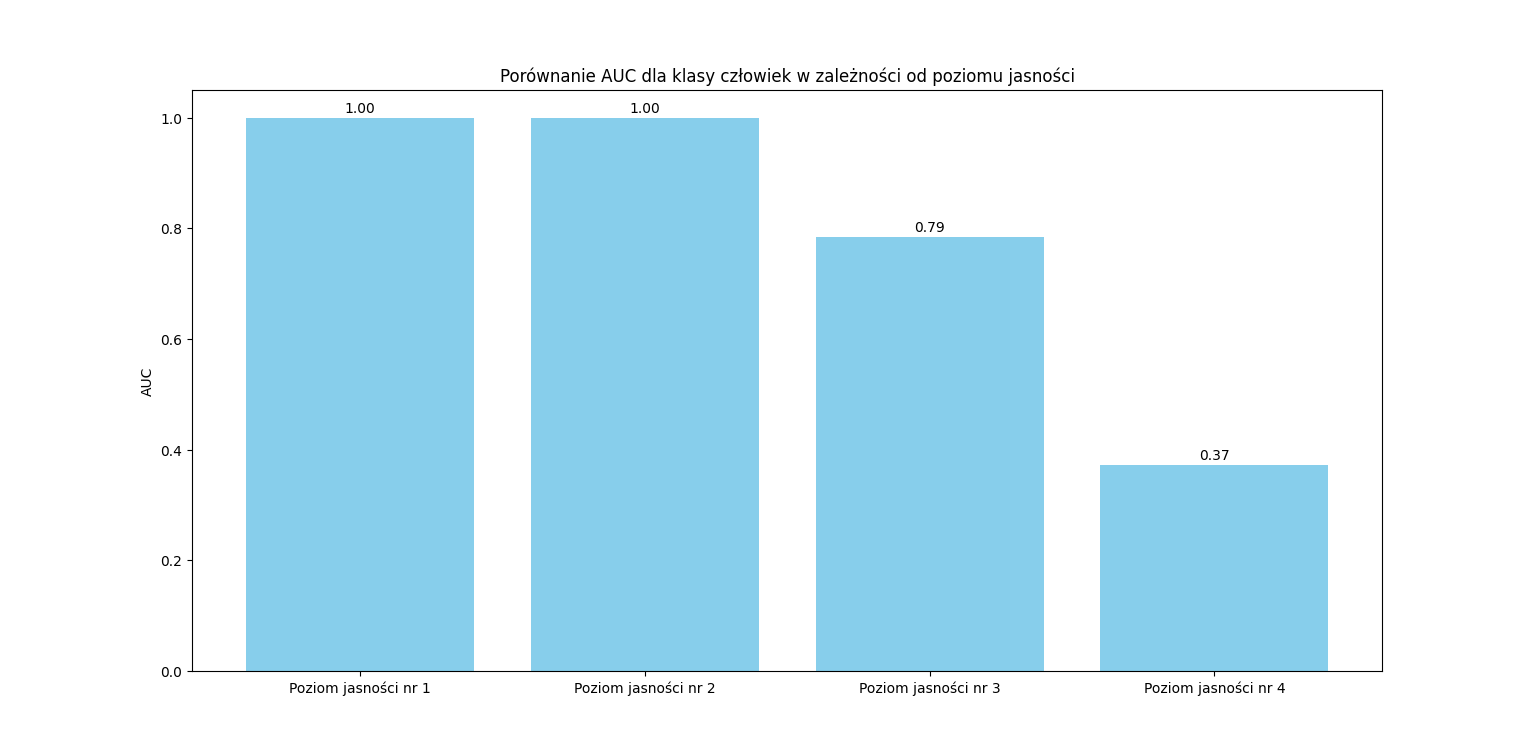
\includegraphics[width=\linewidth]{r_test_dokładności/AUC_charts/porownanieAUC.png}
    \caption{Wykres porównujący wartości AUC dla zbadanych poziomów jasności.}
    \label{fig:AUC}
\end{figure}



\subsection{Analiza wpływu progu ufności na wyniki detekcji}



\section{Test poziomu generalizacji modelu}
\label{sec:test-2}
W tej sekcji zbadano jak dobrze model radzi sobie z różnymi obiektami należącymi do tej samej klasy. Umiejętność generalizacji zostanie sprawdzona na przykładzie klasy \emph{krzesło} (ang. \emph{chair}). Użyte obiekty to krzesło oraz fotel dla graczy (dalej zwany fotelem). Nazwy angielskie tych obiektów to kolejno \emph{chair} i \emph{gaming chair}, jest to ważne, ponieważ klasy COCO zostały stworzone według angielskiego nazwenictwa, na którego podstawie przypisuje się rózne warianty obiektów do jednej klas.  W badaniu tym porównano wyniki dla krzesła i fotela w funkcji progu ufności dla wszystkich (czterech) poziomów ośwetlenia. Do testu wykorzystano osiem filmów -- cztery z widocznym krzesłem i człowiekiem, cztery z widocznym fotelem i człowiekiem. Wartości jasności i nasycenia dla każdego filmu ukazono w tabeli \ref{tab:jasnosc-krzeslo-fotel}. Wygląd nagranego pomieszczenia wraz z nagranym obiektem dla różnych poziomów oświetlenia ukazano na rysunku \ref{fig:chair_grid} (człowiek, krzesło) i 
\ref{fig:game_grid} (człowiek fotel). 
% Please add the following required packages to your document preamble:
% \usepackage{multirow}
\begin{table}[H]
    \centering
    \caption{Jasność i nasycenie dla wszystkich filmów. Pogrubiona czcionka oznacza obiekt należący do analizowanej klasy.}
    \begin{tabular}{|c|c|c|c|}
    \hline
    Poziom   oświetlenia & Obecne obiekty                                & Jasność & Nasycenie \\ \hline
    \multirow{2}{*}{1}   & człowiek,   
    \textbf{krzesło} & 149.92  & 119.07    \\ \cline{2-4} 
                         & człowiek, \textbf{fotel}     & 152.68  & 111.47    \\ \hline
    \multirow{2}{*}{2}   & człowiek,   \textbf{krzesło} & 139.14  & 90.71     \\ \cline{2-4} 
                         & człowiek, \textbf{fotel}     & 133.77  & 83.29     \\ \hline
    \multirow{2}{*}{3}   & człowiek,   \textbf{krzesło} & 38.91   & 132.31    \\ \cline{2-4} 
                         & człowiek, \textbf{fotel}     & 38.12   & 124.31    \\ \hline
    \multirow{2}{*}{4}   & człowiek,   \textbf{krzesło} & 25.3    & 100.8     \\ \cline{2-4} 
                         & człowiek, \textbf{fotel}     & 24.88   & 108.5     \\ \hline
    \end{tabular}
    \label{tab:jasnosc-krzeslo-fotel}
    \end{table}

Tak jak to wspomniano (podrozdział \ref{sec:zrodlo_wideo}), badane obiekty są statyczne i były obecne przez wszystkie klatki każdego filmu. Dlatego też metryki FP i TN są zawsze zerowe. Do tego badania można jednak ponownie skorzystać z TPR, ponieważ metryka ta bazuje jedynie na TP i FN. TPR jest alternatywnie nazywane czułościa i to badanie tak będzie się do niej odwoływać. Czułość dla fotela i krzesła jest zestawiona w funkcji progu ufności dla kolejnych poziomów oświetlenia (wykresy na rysnkach \ref{fig:chair-game-1}, \ref{fig:chair-game-2}, \ref{fig:chair-game-3}, \ref{fig:chair-game-4}). Porównano również poziomy oświetlenia dla konkretnego obiektu -- \ref{fig:all_bright_chair} (krzesło), \ref{fig:all_bright_game} (fotel). 

Wyniki dla każdego poziomu oświetlenia okazały się być lepsze dla krzesła. Przyczyn można upatrywać w dwóch źródłach: po pierwsze, zdecydowanie ciemniejszy kolor fotela jest ciężej wykrywany w coraz ciemniejszym pomieszczeniu. Po drugie, model COCO mógł być wytrenowany dla mniejszej liczby foteli tego typu.

Odnośnie przyczyny pierwszej, można dostrzec zauważalny spadek skuteczeności klasyfikacji na niższych poziomach oświetlenia od poziomu 1. Stało sie tak, pomimo że poziom 2 został uznany za poziom dobrej widoczności -- fotel jest wyraźnie wyszczególniony. Przyczyną może być np. niska jakość nagranego filmu, w tym zakłócenia. 

Podsumowując, stwierdzono, iż model nie generalizuje dobrze klasy \emph{krzesło}. Samo badanie nie świadczy, iż generalizacja YOLOv8n ma podobną jakość w przypadku innych klas. Interesującym rozszerzeniem badań byłoby zbadanie klas niestetycznych, czego nie udało się zrealizować przez wzgląd na osobisty brak takich obiektów. 

\begin{figure}[H]
    \centering
    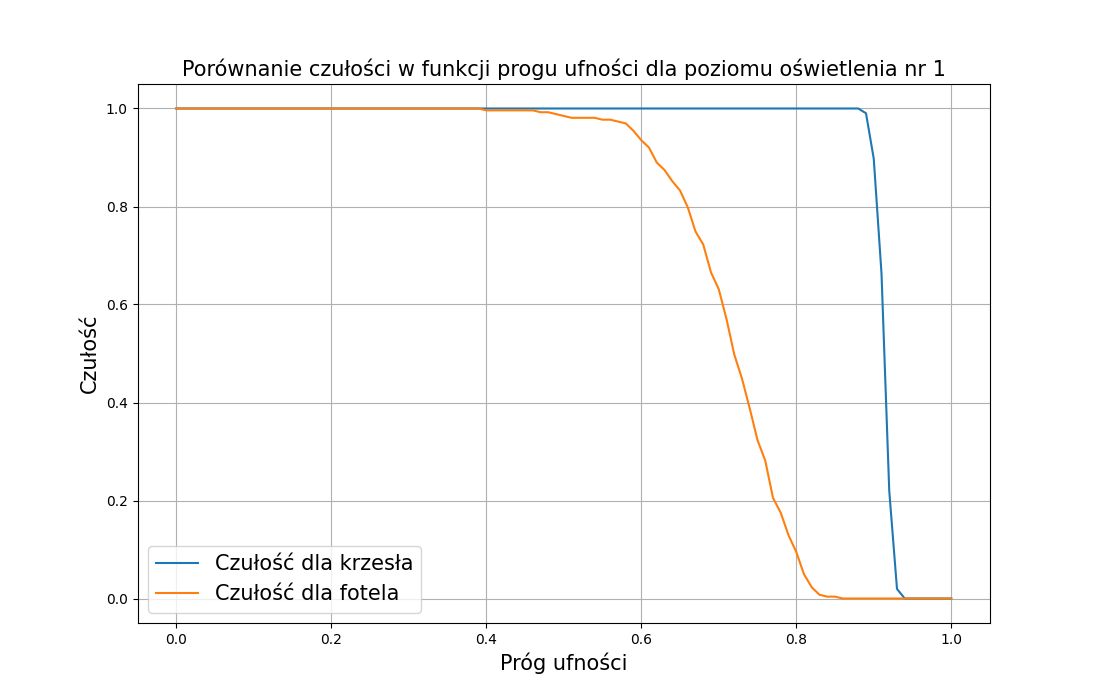
\includegraphics[width=\linewidth]{r_test_dokładności/chair_charts/1.png}
    \caption{Porównanie czułości w funkcji progu ufności dla krzesła i fotela. Poziom oświetlania nr 1.}
    \label{fig:chair-game-1}
\end{figure}

\begin{figure}[H]
    \centering
    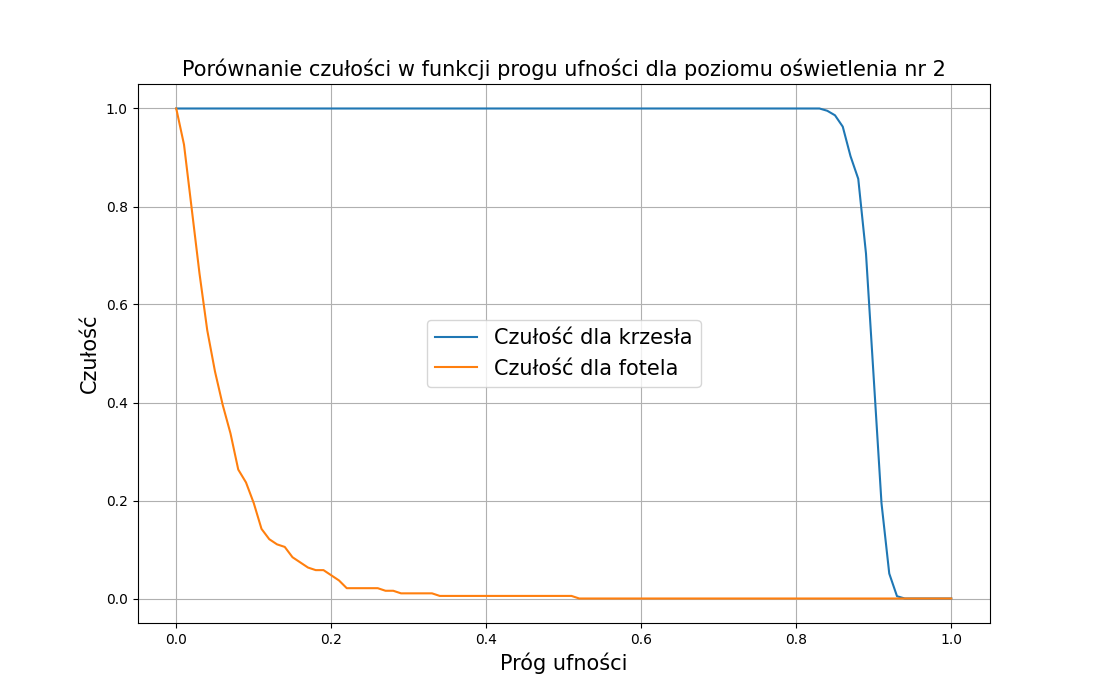
\includegraphics[width=\linewidth]{r_test_dokładności/chair_charts/2.png}
    \caption{Porównanie czułości w funkcji progu ufności dla krzesła i fotela. Poziom oświetlania nr 2.}
    \label{fig:chair-game-2}
\end{figure}

\begin{figure}[H]
    \centering
    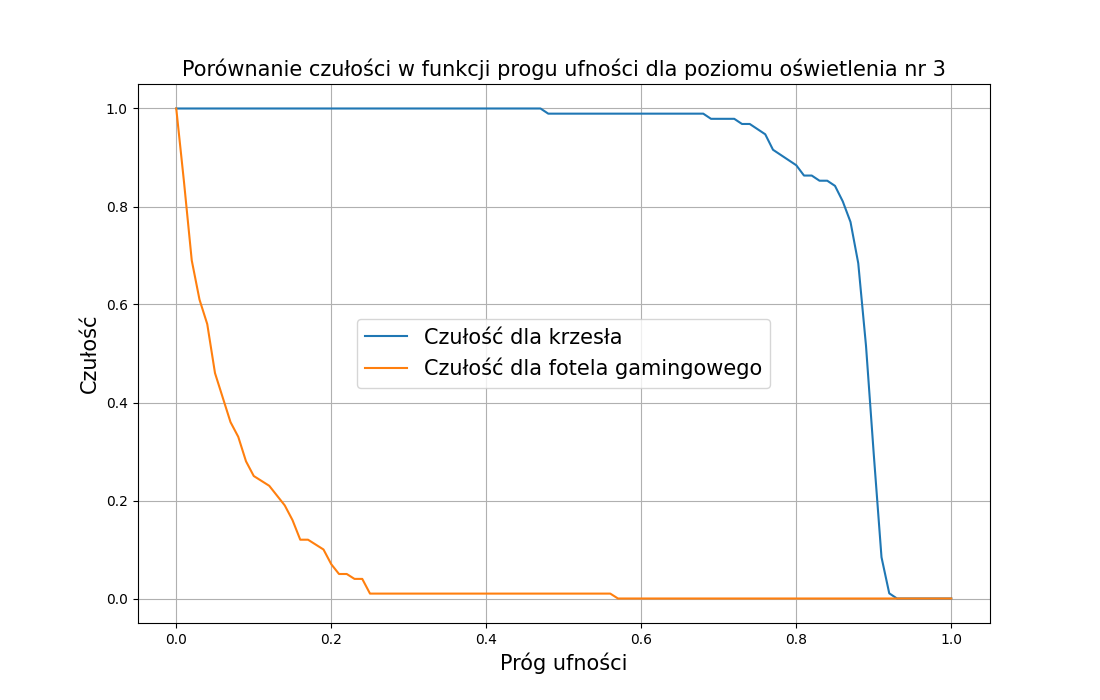
\includegraphics[width=\linewidth]{r_test_dokładności/chair_charts/3.png}
    \caption{Wykres do porównania czułości w funkcji progu ufności dla krzesła i fotela. Poziom oświetlania nr 3.}
    \label{fig:chair-game-3}
\end{figure}

\begin{figure}[H]
    \centering
    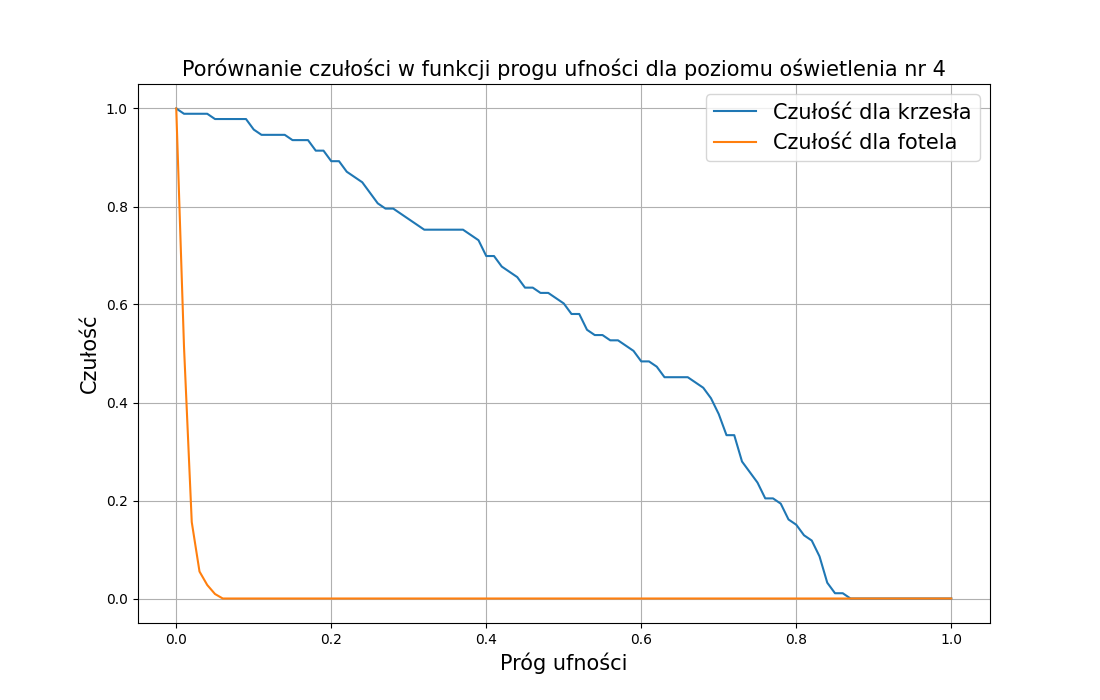
\includegraphics[width=\linewidth]{r_test_dokładności/chair_charts/4.png}
    \caption{Wykres do porównania czułości w funkcji progu ufności dla krzesła i fotela. Poziom oświetlania nr 4.}
    \label{fig:chair-game-4}
\end{figure}

\begin{figure}[H]
    \centering
    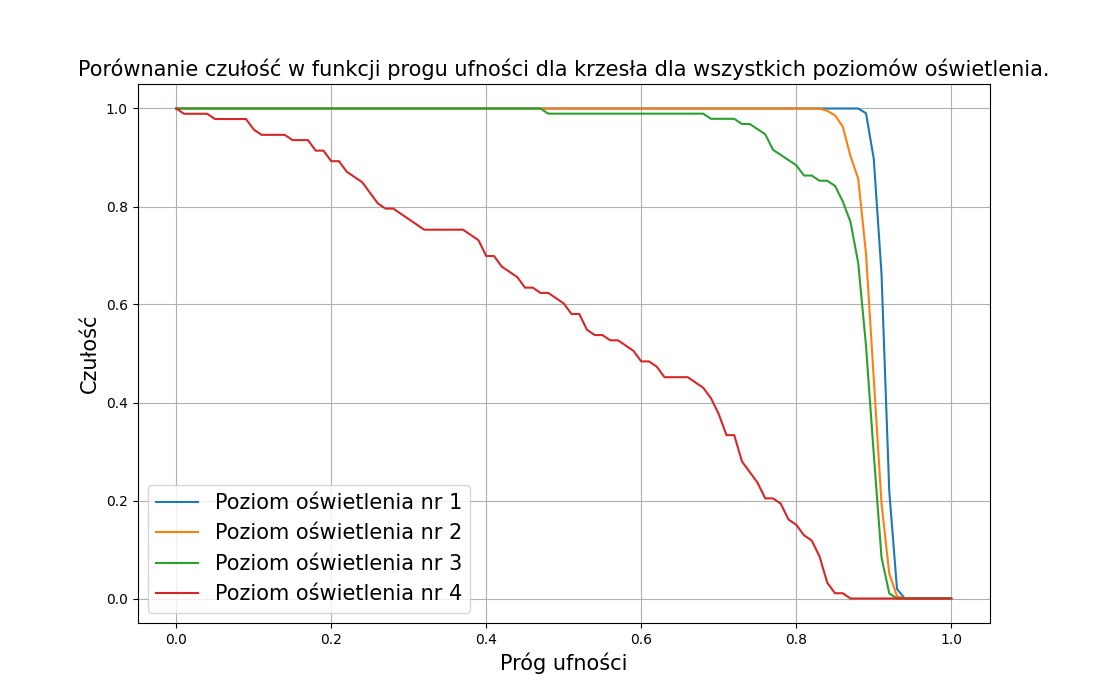
\includegraphics[width=\linewidth]{r_test_dokładności/chair_charts/chair.png}
    \caption{Wykres do porównania czułości w funkcji progu ufności dla wszystkich poziomów oświetlania. Obiekt --  krzesło.}
    \label{fig:all_bright_chair}
\end{figure}

\begin{figure}[H]
    \centering
    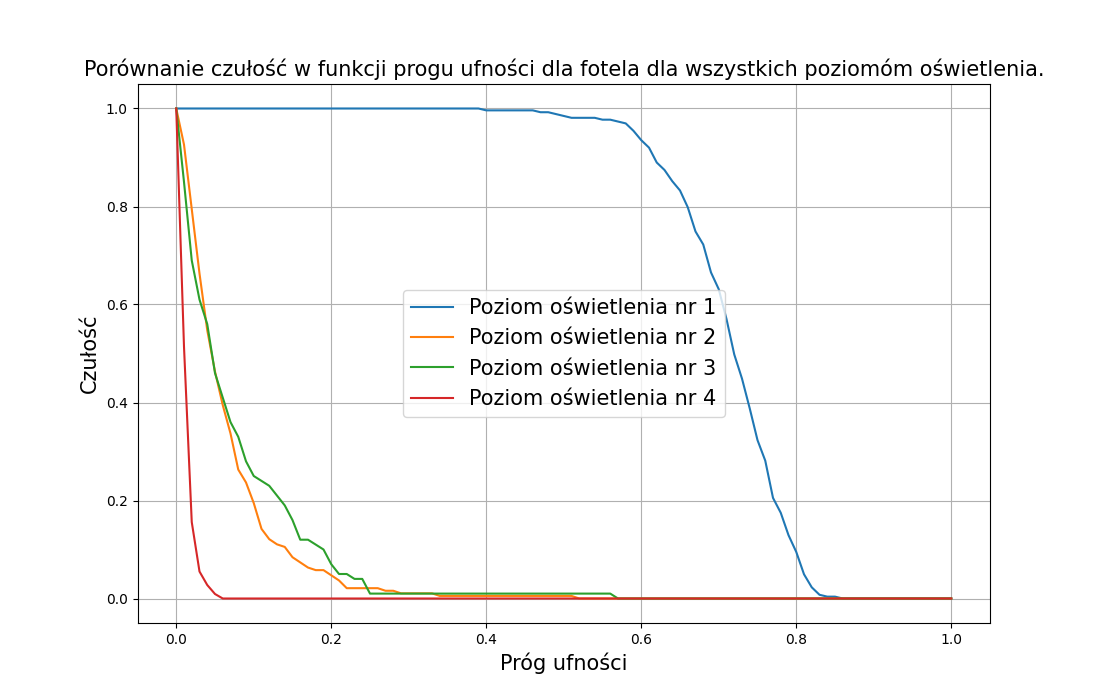
\includegraphics[width=\linewidth]{r_test_dokładności/chair_charts/gaming-chair.png}
    \caption{Wykres do porównania czułości w funkcji progu ufności dla wszystkich poziomów oświetlania. Obiekt --  fotel.}
    \label{fig:all_bright_game}
\end{figure}


\chapter{Podsumowanie}
\label{chap:podsumowanie}
Celem pracy było zaprojektowanie systemu alarmującego w sposób audio-wizualny w sytuacji wykrycia obiektów z podzbioru dostępnych klas ustawionego przez użytkownika. Ponadto należało przeprowadzić badania szybkości systemu oraz badanie dokładności problemu detekcji obiektów dla wybranego modelu sztucznej inteligencji.

Postawione wymagania pracy udało się zrealizować, a do implementacji systemu wykorzystano model YOLOv8n.

Testy szybkości przeprowadzone na zasobach sprzętowych posiadanych przez przeciętnego użytkownika wykazały zadowalające wyniki oraz przybliżoną wydajność dla różnych ustawień rozdzielczości kamery. Badania pokazały, więc realną możliwość użycia systemu w warunkach oświetlenia uznanych za wystarczające w badaniu modelu detekcji przez osobę nie posiadającą zasobów na zakup specjalistycznego systemu np. w celu monitoringu swojej posiadłości.
W przypadku w.w. warunków oświetlenia, badania modelu wykazały bardzo dobrą skuteczność klasyfikacji ludzi w ruchu, a co za tym idzie alarmowania dźwiękowego dla scen z pojedyńczą liczbą obecnych obiektów, w sytuacji dobrze oświetlonych, widocznych konturów człowieka. Przykładem użycia systemu w w.w. warunkach oświetlenia mógłby być scenariusz do alarmowania przejścia obiektu przez wejście do pomiesczenia -- scenariusz podoby do scenariusza testowego.  


Ze względu na brak zasobów sprzętowych o parametrach odpowiadających warunkom profesjonalnego użycia tego typu systemów nie było możliwości porówania niniejszego oprogramowania do istniejących rozwiązań. Jest to natomiast punkt, od którego interesująco byłoby rozpocząć kolejne badania, kładąc szczególny nacisk na wykorzystanie kamery o możliwości dostarczania większej liczby klatek na sekundę, gdyż użycie takiej technologii mogłoby przyśpieszyć działanie wolniejszych modułów systemu i zmienić charakterystykę wyników. Możnaby również powielić przeprowadzone badania -- modelu oraz szybkości systemu -- lecz dla innych rozmiarów modelu YOLOv8.  

%\show\chapter
%\show\section
%\show\subsection

%\showthe\secindent
%\showthe\beforesecskip
%\showthe\aftersecskip
%\showthe\secheadstyle
%\showthe\subsecindent
%\showthe\beforesubsecskip
%\showthe\aftersubsecskip
%\showthe\subseccheadstyle
%\showthe\parskip

% LITERATURA (zostanie wygenerowana automatycznie)
%UWAGA: bibliotekê referencji nale¿y przygotowaæ samemu. Dobrym do tego narzêdziem jest JabRef.
%       JabRef oferuje jednak wiêksz¹ liczbê typów rekordów ni¿ obs³uguje BibTeX.
%       Proszê nie deklarowaæ rekordów o typach nieobs³ugiwanych przez BibTeX.
%       Formatowania wykazu literatury i cytowañ odbywaæ siê ma zgodnie z zadeklarowanym stylem.
%       Zalecane s¹ style produkuj¹ce numeryczne cytowania (w postaci [1], [2,3]).
%       Takim stylem jest np. plabbrv
\bibliographystyle{plabbrv}
%\bibliographystyle{unsrt} 
%       Aby zapanowaæ nad odstêpami w wykazie literatury mo¿na pos³u¿yæ siê poni¿sz¹ komend¹
\setlength{\bibitemsep}{2pt} % - zacieœnia wykaz
%       Pozycja Literatura pojawia siê w spisie treœci nieco inaczej ni¿ spisy rysunków, tabel itp.
%       Aby zachowaæ w³aœciwe odstêpy nale¿y u¿yæ poni¿szej komendy
\addtocontents{toc}{\addvspace{2pt}} % ustawiamy odstêp w spisie treœci przed pozycj¹ Literatura 
%       Nazwê pliku przygotowanej biblioteki wpisuje siê bez rozszerzenia .bib
%       (linia poni¿ej za³aduje rekordy z pliku "dokumentacja.bib")
\bibliography{dokumentacja}
\appendix
%\chapter{Instrukcja wdrożeniowa}
Pliki źródłowe projektu zostały umieszczone w zdalnym repozytorium kodu na stonie github. 
Link do repozytorium: \url{https://github.com/Quarol/Praca-inzynierska.git}

Użytą wersją języka Python jest Python 3.12.4. Aby wykorzystać zaprojektowany system, należy ją zainstalować.

Repozytorium składa się z dwóch plików wykonywalnych (\emph{main.py}, \emph{install\_requirements.py}) oraz dwóch folderów -- \emph{assets} oraz \emph{detector}. Struktura pokazana na ryskunku \ref{fig:repo}.
Folder \emph{assets} zawiera plik dźwiękowy służący jako alarm w systemie. Folder \emph{detector} zawiera wsysztkie pliki źródłowe z opisanymi komponentami systemu.
Plik \emph{install\_requirements.py} to skrypt służący do instalacji wszystkich wykorzystanych modułów języka Python w użytych wersjach.
Plik \emph{main.py} jest to plik uruchamiający aplikację.

W celu instalacji modułów, a następnie uruchomieniu programu należy najpierw uruchomić plik \emph{install\_requirements.py}, a następnie \emph{main.py}. Pliki można uruchomić korzystając ze środowiska programistycznego lub poprzez komendy w terminalu. Komendy mogą różnić się w zależności od systemu operacyjnego oraz sposobu instalacji Pythona. W systemie windows zazwyczaj używa się komendy \emph{python}, przedstawionej na listingu \ref{lst:python_d}, zaś w systemie linux -- \emph{python3} (listing \ref{lst:python3}).

\begin{lstlisting}[caption={Komendy do instalacji modułów oraz uruchomienia aplikacji nr 1.}, label={lst:python_d}]
python install_requirements.py
python main.py
\end{lstlisting}

\begin{lstlisting}[caption={Komendy do instalacji modułów oraz uruchomienia aplikacji nr 2.}, label={lst:python3}]
python3 install_requirements.py
python3 main.py
\end{lstlisting}

\begin{figure}[H]
    \centering
    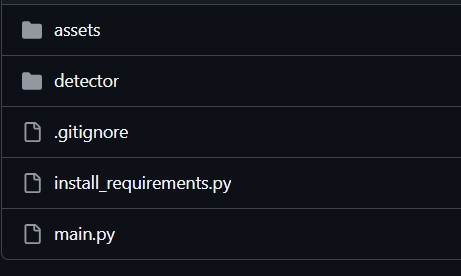
\includegraphics[width=0.55\linewidth]{_repo.jpg}
    \caption{Struktura repozytorium.}
    \label{fig:repo}
\end{figure}




% Jeœli w pracy pojawiaæ siê ma indeks, nale¿y odkomentowaæ poni¿sze linie
%%\chapterstyle{noNumbered}
%%\phantomsection % sets an anchor
%%\addcontentsline{toc}{chapter}{Indeks rzeczowy}
%%\printindex

\end{document}
